\documentclass[a4paper,titlepage]{article}

\usepackage[T1]{fontenc}
\usepackage[utf8]{inputenc}
\usepackage[italian]{babel}
\usepackage[maxfloats=50]{morefloats}
\usepackage{url}
\usepackage{verbatim}
\usepackage{titlepic}
\usepackage{graphicx}
\usepackage{algorithm}
\usepackage{algorithmic}
\usepackage{amsmath}
\usepackage{listings}
\usepackage{subcaption}
\usepackage{adjustbox}
\usepackage{hyperref}
%\usepackage{syntonly}

%\syntaxonly
%\includeonly{}

\lstset{
	language=C,
	frame=single,
	basicstyle=\footnotesize,
	tabsize=3,
	inputencoding=utf8,
	literate={==}{= =}{3}
}
\pdfminorversion=7      %pdf expected version 1.7
\pagestyle{headings}



\begin{document}

\titlepic{
\includegraphics[width=2.5cm]{figures/uniroma2}}

\title{
  Performance Modeling Of Computer Systems And Networks\\[20pt]
  Relazione Progetto 2017/18
}
\author{
  Simone Falvo\\
  \texttt{smvfal@gmail.com}
}

\date{}


\maketitle

%\input{sections/abstract}

\tableofcontents
\newpage

\section{Introduzione}
In questa relazione viene descritta una possibile soluzione ad un problema di
edge computing in cui è richiesto di ottimizzare le prestazioni di un sistema di
computazione cloud, calibrando i parametri di un algoritmo per l'inoltro di task
utente verso un cloudlet ed un server remoto.

Il sistema è in grado di eseguire task di due diverse classi in un cloudlet,
situato ad un ``hop'' di distanza dall'utente, fintanto che le risorse lo
consentono, altrimenti vengono inoltrati ed eseguiti in un server remoto.
Inoltre, se la somma del numero di job presenti nel cloudlet è uguale al valore
di soglia S e se vi è almeno un job di classe 2 in esecuzione, questo viene
fatto migrare dal cloudlet al server remoto per far posto ad un task di classe 1
in arrivo, che ha una maggiore ``priorità'' di esecuzione nel cloudlet.\\
L'obbiettivo principale è quello di trovare il valore ottimale del parametro S
affinché sia minimizzato il tempo di risposta medio.

Il problema è stato affrontato definendo un modello a code per il sistema in
modo tale da poter valutare, tramite l'analisi e la simulazione, i tempi di
risposta e le altre metriche di performance come il throughput e la popolazione
media.\\ 
Il modello è stato validato analiticamente tramite lo studio dello stato del
sistema a regime, calcolandone la distribuzione stazionaria e valutando le
metriche di interesse in relazione ai possibili scenari.\\ 
La simulazione è stata realizzata implementando in linguaggio C un programma
basato su eventi ed i risultati sono stati raccolti ed elaborati utilizzato il
metodo ``batch means'' per avere una stima del comportamento del sistema a
regime.

Nel seguito di questo documento verranno presentati i vari modelli di
astrazione del sistema con i risultati che ne derivano, ed infine verrà fatto un
cofronto in relazione ai possibili scenari analizzati.

\section{Modello Concettuale}
Nel modello concettuale il sistema viene descritto come un sistema di code
connesse tra loro (figura~\ref{conceptual}), di quest'ultimo si distinguono i
seguenti componenti:
\begin{itemize}
\item[\textbf{Cloudlet}:] nodo del sistema che comprende un numero $N$ di server
senza coda che operano in parallelo con tassi di servizio specifici per classi
di job.
\item[\textbf{Cloud}:] nodo del sistema che comprende un numero infinito di
server senza coda che operano in parallelo con tassi di servizio specifici per
classi di job.
\item[\textbf{Centro di setup}:] nodo del sistema che modella la fase di setup
di un job interrotto, composto da un numero infinito di server senza coda che
operano in parallelo con un tasso di servizio pari a $1/E[S_{setup}]$. Un job
interrotto transita per questo centro prima di prendere servizio nel cloud ed il
tempo ivi trascorso corrisponde al tempo necessario alla ri-esecuzione del job.
\item[\textbf{Controllore}:] componente che implementa la logica di routing in
base all’occupazione del cloudlet tenendo conto del parametro di soglia $S$, non
costituisce un centro di servizio in quanto la sua funzione è limitata
all'inoltro dei job.
\end{itemize} 
%
\begin{figure}[!h]
\centering
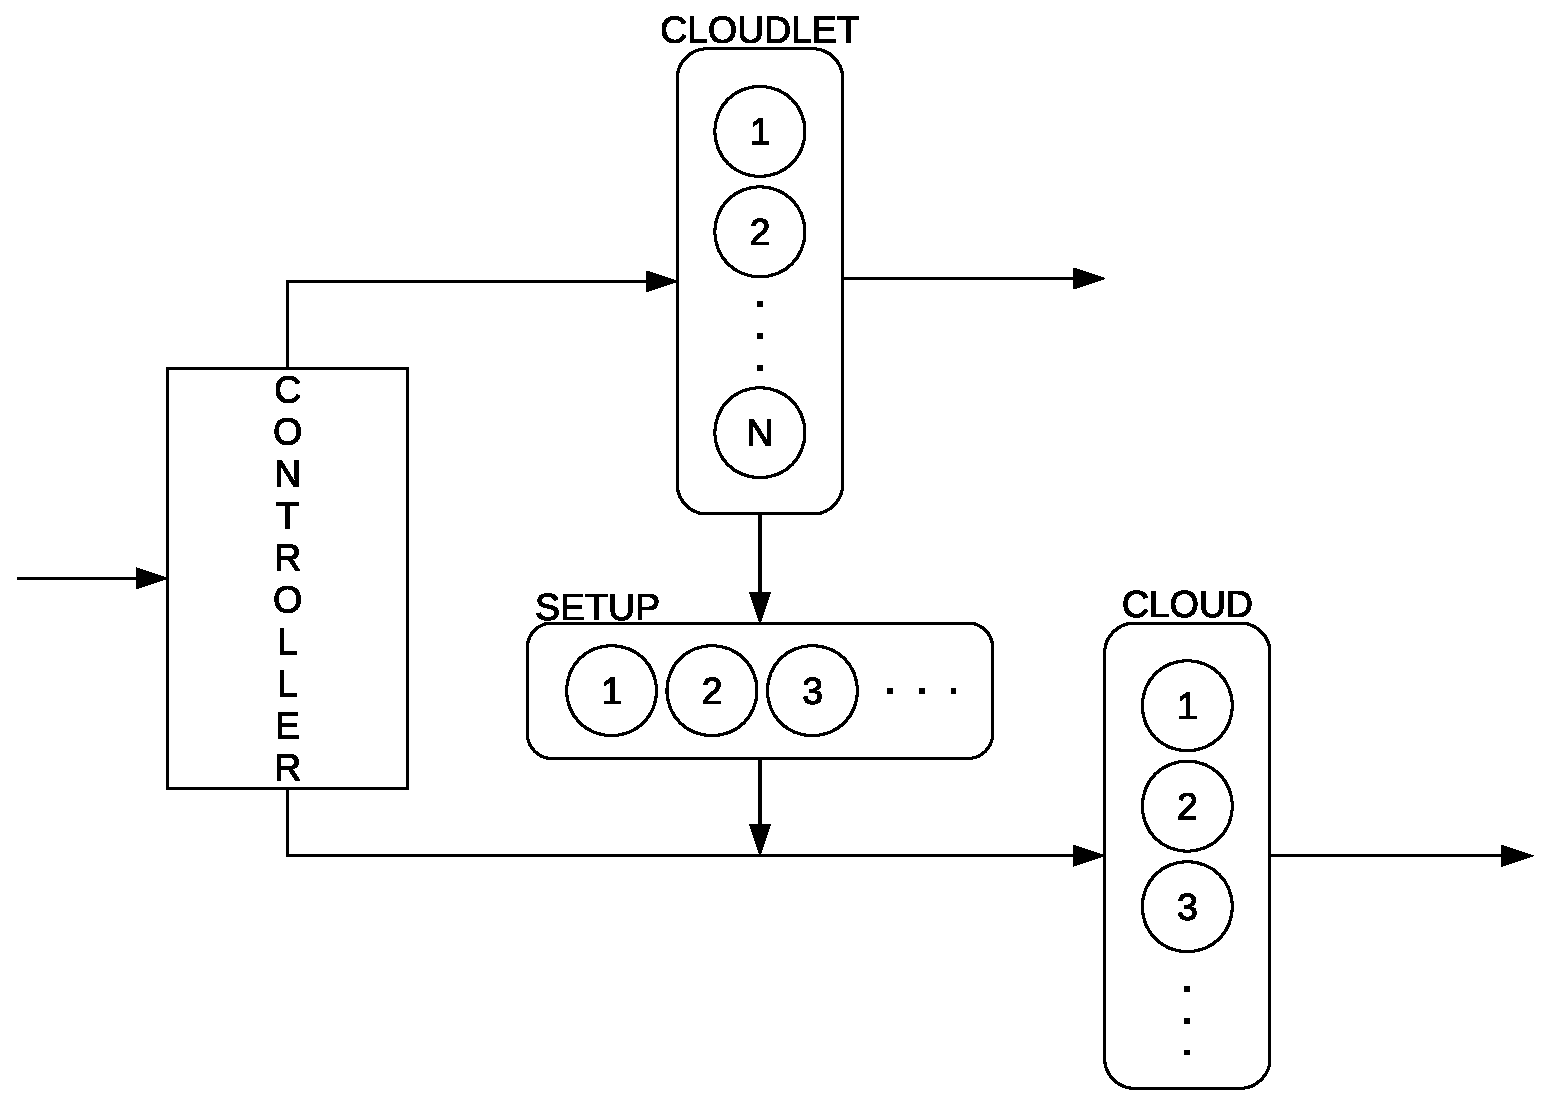
\includegraphics[width=0.7\textwidth]{figures/conceptual}
\caption{Modello concettuale del sistema}
\label{conceptual}
\end{figure}
%
Ogni job che arriva al sistema passa prima per il controllore, il quale decide
quale deve essere il nodo di esecuzione (cloud o cloudlet). Se arriva un job di
classe 1 ed il cloudlet si trova nella condizione per cui almeno un suo server
ha in esecuzione un job di classe 2 e la somma dei job presenti ha raggiunto il
valore di soglia $S$, allora tale server deve sospendere il job e sostituirlo con
quello appena arrivato di classe 1. Il job di classe 2 interrotto verrà poi
inoltrato al server remoto (cloud), non prima però di aver trascorso un tempo
necessario alla propria riesecuzione sul nuovo nodo, tale fase è modellata
assumendo che il job venga eseguito in un centro intermedio (centro di setup).

\section{Modello di Specifica}
In questo modello vengono definite le variabili e le equazioni necessarie al
calcolo delle metriche, inoltre viene descritta la logica con cui il sistema
evolve a seguito degli eventi che si verificano ed i vincoli a cui esso deve
sottostare.
%
%
\subsection{Variabili}
Di principale interesse sono le variabili che compongono lo stato del sistema,
ovvero quelle che lo caratterizzano completamente, esse tengonono conto del
numero di job in servizio suddivisi per classe e per nodo di esecuzione ad ogni
istante di tempo e sono indicate nella tabella~\ref{state}.
%
\begin{table}[!h]
\begin{tabular}{c|l}
{$n_1^{clet}(t)$}  & numero di job di classe 1 nel cloudlet al tempo $t$\\
{$n_2^{clet}(t)$}  & numero di job di classe 2 nel cloudlet al tempo $t$\\
{$n_1^{cloud}(t)$} & numero di job di classe 1 nel cloud al tempo $t$\\
{$n_2^{cloud}(t)$} & numero di job di classe 2 nel cloud al tempo $t$\\
{$n_{setup}(t)$}   & numero di job in fase di setup al tempo $t$\\
\end{tabular}
\centering
\caption{Variabili che compongono lo stato del sistema}
\label{state}
\end{table}
%
Le altre variabili utili al calcolo delle statistiche del sistema sono indicate
nella tabella~\ref{vars} e riguardano i tempi di risposta ed i completamenti,
sempre suddivise per classe e nodo di esecuzione.
%
\begin{table}[!h]
\begin{tabular}{c|l}
{$s_{1,i}^{clet}$}     & tempo di servizio dell’i-esimo job di classe 1 eseguito
nel cloudlet \\[2pt]
{$s_{2,i}^{clet}$}     & tempo di servizio dell’i-esimo job di classe 2 eseguito
nel cloudlet \\[2pt]
{$s_{1,i}^{cloud}$}    & tempo di servizio dell’i-esimo job di classe 1 eseguito
nel cloud \\[2pt]
{$s_2^{cloud,i}$}      & tempo di servizio dell’i-esimo job di classe 2 eseguito
nel cloud \\[2pt]
{$s_{intr,i}^{clet}$}  & tempo di servizio nel cloudlet dell’i-esimo job
interrotto \\[2pt]
{$s_{intr,i}^{cloud}$} & tempo di servizio nel cloud dell’i-esimo job interrotto
\\[2pt]
{$s_i^{setup}$}        & tempo di setup dell’i-esimo job interrotto \\[2pt]
{$c_1^{clet}(t)$}      & numero di job di classe 1 completati nel cloudlet al
tempo $t$ \\[2pt]
{$c_2^{clet}(t)$}      & numero di job di classe 2 completati nel cloudlet al
tempo $t$ \\[2pt] 
{$c_1^{cloud}(t)$}     & numero di job di classe 1 completati nel cloud al tempo
$t$ \\[2pt] 
{$c_2^{cloud}(t)$}     & numero di job di classe 2 completati nel cloud al tempo
$t$ \\[2pt]
{$n_{intr}(t)$}        & numero di job interrotti al tempo $t$ \\
\end{tabular}
\centering
\caption{Variabili tempi di servizio e completamenti}
\label{vars}
\end{table}
%
%
\subsection{Vincoli}
Una volta definito lo stato del sistema e le variabili che lo compongono è
necessario definire anche come esse sono relazionate ed i vincoli a cui sono
sottoposte.
\begin{enumerate}
\item Ad ogni istante di tempo $t$ devono valere le seguenti condizioni:
\begin{eqnarray*}
n_1^{clet}(t) + n_2^{clet}(t) & \leq N & \\
n_1^{clet}(t) + n_2^{clet}(t) & \leq S & \qquad \textrm{se } n_2^{clet}(t) > 0
\end{eqnarray*}
\item Stato iniziale ($t=t_{start}$):
\begin{eqnarray*}
n_1^{clet}(t) = n_2^{clet}(t) = n_1^{cloud}(t) = n_2^{cloud}(t) = n_{setup}(t) &=& 0 
\\
c_1^{clet}(t) = c_2^{clet}(t) = c_1^{cloud}(t) = c_2^{cloud}(t) = c_{setup}(t) &=& 0
\end{eqnarray*}
\item Il primo evento deve essere un arrivo
\item Dopo l’arrivo di un numero prefissato di job, i successivi arrivi vengono
ignorati e non più processati.  Il processo di arrivo si interrompe quando viene
processato un numero prefissato di job.  L’ultimo evento corrisponde al
completamento dell’ultimo job.
\item La selezione dei server all’interno di un nodo non è regolata da nessun
algoritmo, poiché metriche relative ai singoli server non sono rilevanti ai fini
dell’applicazione.  
\end{enumerate}
%
%
\subsection{Metriche}
\subsubsection{Tempi di risposta}
Poiché i nodi del sistema sono sprovvisti di code, i tempi medi di risposta
corrispono ai tempi medi di servizio, il calcolo viene quindi ridotto al
rapporto tra la somma dei tempi di servizio sperimentati dai job in esame e la
loro quantità, pertanto, per prima cosa è utile calcolare le somme dei
tempi:
\begin{displaymath}
s_j^{clet} = \displaystyle \sum_{i=1}^{c_j^{clet}(t_{stop})} s_{j,i}^{clet} 
\qquad\quad
s_j^{cloud} = \displaystyle \sum_{i=1}^{c_j^{cloud}(t_{stop})} s_{j,i}^{cloud}
\qquad \quad j = 1, 2 
%s_{intr}^{clet} = \sum_{i=1}^{n_{intr}(t_{stop})} s_{intr,i}^{clet} &\quad&
%s_{intr}^{cloud} = \sum_{i=1}^{n_{intr}(t_{stop})} s_{intr,i}^{cloud} \ \qquad
%\ s_{setup} = \sum_{i=1}^{n_{intr}(t_{stop})} s_i^{setup} 
\end{displaymath}
\begin{displaymath}
s_{intr} = \sum_{i=1}^{n_{intr}(t_{stop})} (s_{intr,i}^{clet} +
s_{intr,i}^{cloud} + s_i^{setup})
\end{displaymath}
%
Con queste formule si è ottenuta la somma dei tempi di servizio dei job
suddivisi per classe e nodo di esecuzione, ed anche una relativa esclusivamente
ai job interrotti in cui vengono sommati i tempi associati ai differenti nodi
che percorrono (cloudlet, setup e cloud).

È importante notare che il numero di job coinvolti è relativo ad un'istante di
tempo corrispondente alla fine della finestra di osservazione $[t_{start};
t_{stop}]$, ove si è posto per semplicità $t_{start}=0$.

Adesso per il calcolo dei tempi di risposta rimane da fare il rapporto con i
completamenti relativi ai nodi oppure alle classi di interesse.
%
\setlength\arraycolsep{2pt}
\begin{eqnarray}
\label{eq:sjclet}
E[T_j^{clet}] = E[S_j^{clet}] &=& \frac{s_j^{clet}}{c_j^{clet}(t_{stop})}
\ \qquad \ \qquad \ j = 1, 2 
\\[10pt]
\label{eq:sjcloud}
E[T_j^{cloud}] = E[S_j^{cloud}] &=&
\frac{s_j^{cloud}}{c_j^{cloud}(t_{stop})}
\qquad \ \qquad j = 1, 2 
\\[10pt]
\label{eq:sintr}
E[T_{intr}] = E[S_{intr}] & = &
\frac{s_{intr}}{n_{intr}(t_{stop})}
\end{eqnarray}
\begin{eqnarray}
\label{eq:s1}
E[T_1] = E[S_1] & = &
\frac{s_1^{clet} + s_1^{cloud}}{c_1^{clet}(t_{stop}) + c_1^{cloud}(t_{stop})}
\\[10pt]
\label{eq:s2}
E[T_2] = E[S_2] & = &
\frac{s_1^{clet} + s_1^{cloud} + s_{intr}}{c_2^{clet}(t_{stop}) +
c_2^{cloud}(t_{stop})} \\[10pt]
\label{eq:s}
E[T] = E[S] & = &
\frac{s_1^{clet} + s_1^{cloud} + s_2^{clet} + s_2^{cloud} + s_{intr}}
{c_1^{clet}(t_{stop}) + c_1^{cloud}(t_{stop}) + c_2^{clet}(t_{stop}) +
c_2^{cloud}(t_{stop})} 
\end{eqnarray}
%
Nella formula~\ref{eq:sintr} la somma dei tempi di servizio dei job interrotti
viene divisa per il numero di interruzioni, che equivale al numero di
completamenti.\\
Nella formula~\ref{eq:s2}, in cui si calcola il tempo di risposta dei job di
classe 2, vengono considerati i job della suddetta classe che passano
esclusivamente per il cloudlet e per il cloud oltre ai job che subiscono le
interruzioni, ma al denominatore non è presente il numero di job interrotti
$n_{intr}$ perché è già incluso nella variabile $c_2^{cloud}$, essendo tali job
completati nel cloud. Lo stesso discorso vale per la formula~\ref{eq:s}.
%
\subsubsection{Popolazione media}
La popolazione media viene calcolata integrando le variabili in un'intervallo di 
tempo corrispondente alla finestra di osservazione della simulazione e dividendo
per la lunghezza di quest'ultima. Le metriche globali possono essere calcolate
sommando le opportune metriche locali, poiché sono relative tutte allo stesso
intervallo di tempo.
\begin{eqnarray}
\label{eq:njclet}
E[N_j^{clet}] & = &
\frac{1}{t_{stop} - t_{start}} 
\displaystyle \int_{t_{start}}^{t_{stop}} n_j^{clet}(t) \ dt
\qquad j = 1, 2 
\\[10pt]
\label{eq:njcloud}
E[N_j^{cloud}] & = &
\frac{1}{t_{stop} - t_{start}} 
\displaystyle \int_{t_{start}}^{t_{stop}} n_j^{cloud}(t) \ dt
\qquad j = 1, 2 
\\[10pt]
\label{eq:nsetup}
E[N_{setup}] & = &
\frac{1}{t_{stop} - t_{start}} 
\displaystyle \int_{t_{start}}^{t_{stop}} n_{setup}(t) \ dt
\\[10pt]
\label{eq:n1}
E[N_{1}] & = & E[N_1^{clet}] + E[N_1^{cloud}]
\\[10pt]
\label{eq:n2}
E[N_{2}] & = & E[N_2^{clet}] + E[N_2^{cloud}] + E[N_{setup}]
\\[10pt]
\label{eq:nclet}
E[N_{clet}] & = & E[N_1^{clet}] + E[N_2^{clet}]
\\[10pt]
\label{eq:ncloud}
E[N_{cloud}] & = & E[N_1^{cloud}] + E[N_2^{cloud}]
\\[10pt]
\label{eq:n}
E[N] & = & E[N_{cloud}] + E[N_{clet}] + E[N_{setup}] 
\\   & = & E[N_{1}] + E[N_{2}]
\end{eqnarray}
%
Può essere utile ricordare che i job interrotti sono job di classe 2, pertanto
nel calcolo della popolazione media dei job di questa classe nel sistema
(equazione~\ref{eq:n2}), vanno considerati anche i job nel centro di setup.
%
\subsubsection{Throughput}
Il throughput viene calcolato come il numero di job completati in un intervallo
di tempo corrispondente alla finestra di osservazione della simulazione.\\
Come per la popolazione media è sufficiente comporre i vari throughput locali
per ottenere i throughput del sistema, dei singoli nodi oppure delle singole
classi. Per esempio per il calcolo del throghput del sistema
(equazione~\ref{eq:x}) si possono sommare i throughput delle classi oppure i
throughput dei nodi.
\begin{eqnarray}
\label{eq:xjclet}
X_j^{clet} & = & \frac{c_j^{clet}(t_{stop})}{t_{stop} - t_{start}} 
\qquad j = 1, 2 
\\[10pt]
\label{eq:xjcloud}
X_j^{cloud} & = & \frac{c_j^{cloud}(t_{stop})}{t_{stop} - t_{start}} 
\qquad j = 1, 2 
\\[10pt]
\label{eq:xj}
X_j & = & X_j^{clet} + X_j^{cloud}
\qquad j = 1, 2 
\\[10pt]
\label{eq:xclet}
X_{clet} & = & X_1^{clet} + X_2^{clet}
\\[10pt]
\label{eq:xcloud}
X_{cloud} & = & X_1^{cloud} + X_2^{cloud}
\\[10pt]
\label{eq:x}
X & = & X_1 + X_2 = X_{clet} + X_{cloud}
\end{eqnarray}
%%
Il throughput del centro di setup non è particolarmente interessante perché è un
nodo interno che non emette job all'esterno del sistema, funge solo da nodo
intermedio tra cloudlet e cloud, in definitiva il suo throughput non
contriubuisce a quello del sistema.
\subsubsection{Interruzioni}
La percentuale di job interrotti viene calcolata sia rispetto al numero di job di
classe 2 del sistema, sia rispetto al numero di job di classe 2 che passano per
il cloudlet.
\begin{eqnarray}
P_{intr} &=& 
\frac{n_{intr}(t_{stop})}{c_2^{clet}(t_{stop}) + c_2^{cloud}(t_{stop})} \\[10pt]
P_{intr}^{clet} &=& 
\frac{n_{intr}(t_{stop})}{n_{intr}(t_{stop}) + c_2^{clet}(t_{stop})}
\end{eqnarray}
%
\subsection{Eventi}
Lo stato del sistema evolve a seguito di eventi di vario tipo:
\begin{enumerate}
\item{Arrivo di un job di classe 1}
\item{Arrivo di un job di classe 2}
\item{Partenza di un job}
\item{Setup}
\end{enumerate}
%
L'algoritmo~\ref{alg} mostra tale evoluzione e le azioni che vengono intraprese
in ogni possibile caso.\\
In generale ad ogni arrivo viene stabilito il nodo di esecuzione in base allo
stato del cloudlet e vengono aggiornate opportunamente le variabili, nel caso si
debba sostituire un job di classe 2 con uno di classe 1 appena arrivato si
provvede a rimuovere il relativo tempo di servizio $s_2^{clet,k}$
precedentemente aggiunto e a registrare l'ammontare di tempo $s_{intr,k}$ per
cui il job è stato in esecuzione prima che venisse interrotto.  Nel caso in cui
si verifica un evento di partenza viene incrementato la corrispondente variabile
di completamento e nel caso di un evento di setup, il relativo job
precedentemente interrotto può essere finalmente eseguito sul cloud. Si noti
anche che, nell'aggiornamento delle variabili temporali, l'istante $t'$ è
corrisponde al momento in cui si verifica l'evento successivo a quello corrente
che avviene all'istante $t$.
%
\begin{algorithm}[!h]
\centering
\caption{Logica del sistema in base agli eventi}
\label{alg}
\begin{algorithmic}
\STATE \textbf{Arrivo di un job $i$ di classe 1}:
\IF{$n_1^{clet}(t) = N$}
\STATE \emph{esecuzione su cloud}
\STATE $s_1^{cloud} \leftarrow s_1^{cloud} + s_{1,i}^{cloud}$
\STATE $n_1^{cloud}(t') \leftarrow n_1^{cloud}(t) + 1$
\ELSIF{$n_1^{clet}(t) + n_2^{clet}(t) < S$}
\STATE \emph{esecuzione su cloudlet}
\STATE $s_1^{clet} \leftarrow s_1^{clet} + s_{1,i}^{clet}$
\STATE $n_1^{clet}(t') \leftarrow n_1^{clet}(t) + 1$
\ELSIF{$n_2^{clet}(t) > 0$}
\STATE \emph{interruzione e setup job $k$ di classe 2}
\STATE \emph{esecuzione su cloudlet job $i$ di classe 1}
\STATE $s_1^{clet} \leftarrow s_1^{clet} + s_{1,i}^{clet}$
\STATE $s_2^{clet} \leftarrow s_2^{clet} - s_2^{clet,k}$
\STATE $s_{intr} \leftarrow s_{intr} + s_{intr,k}$
\STATE $s_{setup} \leftarrow s_{setup} + s_{setup,k}$
\STATE $n_{setup}(t') \leftarrow n_{setup}(t) + 1$
\STATE $n_1^{clet}(t') \leftarrow n_1^{clet}(t) + 1$
\STATE $n_2^{clet}(t') \leftarrow n_2^{clet}(t) - 1$
\ELSE
\STATE \emph{esecuzione su cloudlet}
\STATE $s_1^{clet} \leftarrow s_1^{clet} + s_{1,i}^{clet}$
\STATE $n_1^{clet}(t') \leftarrow n_1^{clet}(t) + 1$
\ENDIF
\STATE \textbf{Arrivo di un job $i$ di classe 2}:
\IF{$n_1^{clet}(t) + n_2^{clet}(t) \geq S$}
\STATE \emph{esecuzione su cloud}
\STATE $s_2^{cloud} \leftarrow s_2^{cloud} + s_2^{cloud,i}$
\STATE $n_2^{cloud}(t') \leftarrow n_2^{cloud}(t) + 1$
\ELSE
\STATE \emph{esecuzione su cloudlet}
\STATE $s_2^{clet} \leftarrow s_2^{clet} + s_{2,i}^{clet}$
\STATE $n_2^{clet}(t') \leftarrow n_2^{clet}(t) + 1$
\ENDIF
\STATE \textbf{Partenza di un job di classe $j$ dal cloudlet}:
\STATE $c_j^{clet}(t') \leftarrow c_j^{clet}(t) + 1$
\STATE $n_j^{clet}(t') \leftarrow n_j^{clet}(t) - 1$
\STATE \textbf{Partenza di un job di classe $j$ dal cloud}:
\STATE $c_j^{cloud}(t') \leftarrow c_j^{cloud}(t) + 1$
\STATE $n_j^{cloud}(t') \leftarrow n_j^{cloud}(t) - 1$
\STATE \textbf{Setup}:
\STATE \emph{esecuzione su cloud}
\STATE $s_2^{cloud} \leftarrow s_2^{cloud} + s_2^{cloud,i}$
\STATE $n_{setup}(t') \leftarrow n_{setup}(t) - 1$
\STATE $n_2^{cloud}(t') \leftarrow n_2^{cloud}(t) + 1$
\end{algorithmic}
\end{algorithm}
%
%

\section{Modello Computazionale}
Il modello computazionale consiste in un programma di simulazione di tipo
next-event che impiega il metodo ``batch means'' per il calcolo di tutte le
metriche di interesse. 
A questo livello di astrazione del sistema si passa ad implementare tutto ciò
che è stato definito formalmente nel modello di specifica, in particolare in
questa sezione verranno descritte le strutture dati impiegate per la
rappresentazione delle variabili, le funzioni ed i costrutti che realizzano la
logica del sistema, come vengono generati i dati di input ed infine le
metodologie con cui vengono collezionati ed elaborati i dati di output.
%
%
\subsection{Strutture dati}
In primo luogo, vengono definite le strutture dati riguardanti la lista degli
eventi possibili ed il clock che regola il tempo di simulazione, successivamente
quelle che contegono i dati di output ed infine la struttura dati relativa alla
principale entità manipolata nel sistema: il job.
%
\subsubsection{Eventi e clock virtuale}
Ad ogni istante la lista di eventi è così composta:
\begin{itemize}
\item[-]prossimo arrivo job di classe 1
\item[-]prossimo arrivo job di classe 2
\item[-]al più $N$ completamenti di job nel cloudlet
\item[-]$0$ o più completamenti di job nel cloud
\item[-]$0$ o più completamenti di fase di setup dei job interrotti
\end{itemize}
non essendovi un numero finito di eventi da gestire, occorre realizzare la lista
di eventi tramite una struttura dati dinamica, pertanto gli eventi vengono
gestiti tramite una coda prioritaria, ordinata per scadenza, ovvero con una
politica del tipo Least Remaining Time (figura~\ref{eventq}).
%
\begin{figure}[!h]
\centering
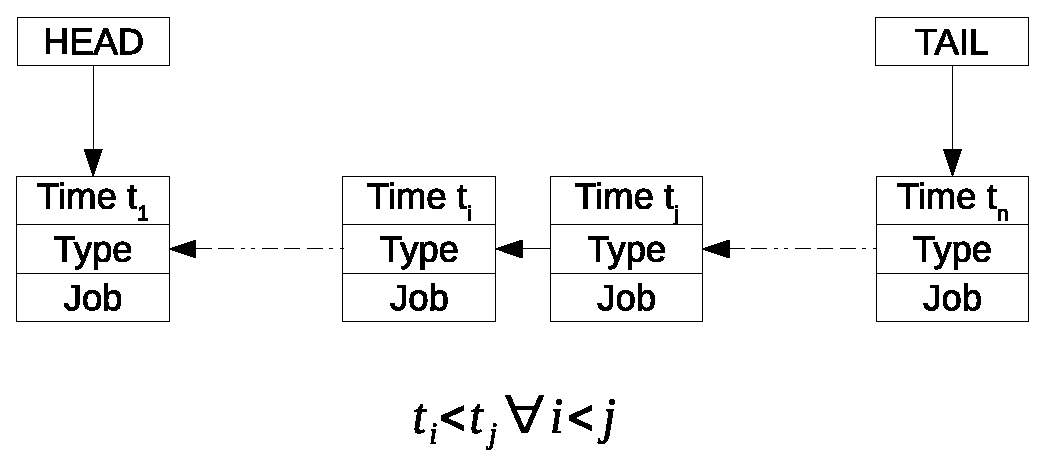
\includegraphics[width=0.7\textwidth]{figures/eventq}
\caption{Coda prioritaria di eventi, ordinata per istante di scadenza}
\label{eventq}
\end{figure}
%
\\Un generico evento è composto dai seguenti campi:
\begin{itemize}
\item L’istante in cui l’evento si verifica
\item La tipologia di evento (arrivo, partenza, setup)
\item Il job associato
\item Un array contenente lo stato del sistema (la sua struttura verrà discussa
più avanti)
\end{itemize}
%
Ogniqualvolta viene creato un evento, questo viene inserito nella coda nella
posizione opportuna tramite un’operazione di \emph{enqueue}, affinché ogni 
operazione di \emph{dequeue} estragga l’evento più imminente.

Il tempo di simulazione è regolato da un clock virtuale che tiene conto
dell’istante corrente e del successivo in modo tale da poter considerare
intervalli di tempo utili per il calcolo di statistiche di tipo time-averaged.

\begin{figure}[!h]
\begin{lstlisting}[title=Impementazione Evento e Clock Virtuale (basic.h)]
struct event {
    double time;
    struct job_t job;
    unsigned int type;
    unsigned int n[4];
};

typedef struct {           /* simulation clock                  */
    double current;        /*   current time                    */
    double next;           /*   next (most imminent) event time */
} clock;
\end{lstlisting}
\end{figure}

%
\subsubsection{Variabili di Output}
I dati che man mano devono essere raccolti durante la simulazione sono
memorizzati in variabili suddivise in base alla tipologia e al nodo di
esecuzione dei job. Per esempio, lo stato del sistema, così come il numero di
arrivi e completamenti, è implementato tramite un array di dimensione 4, di cui
ogni slot corrisponde ad una combinazione classe-nodo a cui il job può essere
associato. 

L’accesso ad uno slot dell’array viene effettuato tramite un indice
che viene calcolato tramite la somma di macro che rappresentano le varie
combinazioni, infatti, se si vuole considerare il numero di job di classe 1 in
esecuzione nel cloud basta accedere all’array tramite l’indice che deriva dalla
somma delle macro J\_CLASS1 e CLOUD ($0 + 2 = 2$). La tabella~\ref{comb}
descrive le possibili combinazioni di macro legate all’indice di accesso.
\begin{table}[!h]
\begin{tabular}{c|c|c|c}
          & CLET & CLOUD & SETUP \\
\hline
J\_CLASS1 & 0    & 2     &       \\
\hline
J\_CLASS2 & 1    & 3     & 4     \\
\end{tabular}
\centering
\caption{Combinazioni per il calcolo dell'indice degli array}
\label{comb}
\end{table}
%
\begin{figure}[!h]
\begin{lstlisting}[title=Definizione macro Nodi e Classi (basic.h)]
 #define J_CLASS1    0           /* job class type 1 */
 #define J_CLASS2    1           /* job class type 2 */
 #define CLET        0           /* cloudlet index   */
 #define CLOUD       2           /* cloud index      */
 #define SETUP       3           /* setup index      */
\end{lstlisting}
\end{figure}
\subsubsection{Task}
Un generico task, anche detto job, viene implementato come una struttura
specifica dotata dei seguenti attributi: 
\begin{itemize}
\item[id]: identificatore univoco necessario ad effettuare un riordino dei job
nel momento in cui vanno considerate le statistiche in un ordine corrispondente
agli istanti di arrivo dei singoli job
\item[class]: specifica la classe del job, può assumere il valori J\_CLASS1 e
J\_CLASS2 (macro definite nel file di configurazione); 
\item[node]: specifica il nodo in cui il job è in esecuzione, può assumere i
valori CLET, CLOUD, SETUP (macro definite nel file di configurazione), che
corrispondono rispettivamente a cloudlet, cloud e nodo di setup; 
\item[service]: array che memorizza i tempi di risposta seguendo la stessa regola
delle combinazioni che riguarda anche lo stato del sistema. Un job di classe 1
in esecuzione nel cloud avrà un tempo di risposta non nullo nello slot relativo,
un job interrotto avrà un tempo di risposta non nullo sia nello slot riguardante
il nodo cloudlet che in quello riguardante il nodo cloud. 
\item[setup]: tempo che un job trascorre in fase di setup. Il valore rimane
nullo nel caso in cui il job non viene interrotto.  
%
\end{itemize}
\begin{figure}[!h]
\begin{lstlisting}[title=basic.h]
struct job_t {
    unsigned long id;
    unsigned int class;
    unsigned int node;
    double service[4];
    double setup;
};
\end{lstlisting}
\end{figure}
%
%
\subsection{Generazione dell'input}
I dati di input della simulazione, corrispondenti ai tempi di interarrivo e di
servizio dei singoli job, vengono generati a runtime in base alle informazioni
note sulle rispettive distribuzioni esponenziali. Per ottenere tali
distribuzioni sono state utilizzate le funzioni delle librerie \emph{rvgs} e
\emph{rngs} di \emph{Steve Park} e \emph{Dave Geyer} descritte in \cite{leemis}.

La funzione \emph{GetArrival()}, ogniqualvolta viene chiamata, restituisce il
più imminente istante di arrivo tra un job di classe 1 ed uno di classe 2 e
memorizza nella variabile $j$, passata per riferimento, la classe del job in
questione. Tali istanti di arrivo vengono calcolati progressivamente a seguito
della generazione dei tempi di interarrivo tra un job e l’altro, più
precisamente, non appena viene restituito un istante di arrivo relativo al job
di una classe, viene calcolato il successivo per la medesima classe.

La funzione \emph{GetService()} restituisce un valore che deriva dalla
generazione di un tempo di servizio esponenziale con media stabilita in base ai
parametri $j$ e $n$ passati come argomento che indicano rispettivamente la
classe ed il nodo di esecuzione del job.

La funzione \emph{GetSetup()} restituisce semplicemente un valore generato a
partire da una distribuzione esponenziale di media $E[S_{setup}]$.

Le funzioni in questione sono elencate di seguito. Si noti che prima di ogni
chiamata alle funzioni della libreria \emph{rvgs} viene selezionato, tramite la
funzione \emph{SelectStream()}, un flusso di generazione di numeri
pseudo-casuali distinto, affinché sia garantita il più possibile l’indipendenza
tra le sequenze di numeri generate.  
%
\begin{figure}[!h]
\begin{lstlisting}[title=basic.h]
double GetArrival(unsigned int *j)
{
    const double mean[2] = {1/L1, 1/L2};
    static double arrival[2] = {START, START};
    static int init = 1;
    double temp;

    if (init) {
        SelectStream(0);
        arrival[0] += Exponential(mean[0]);
        SelectStream(1);
        arrival[1] += Exponential(mean[1]);
        init=0;
    }

    if (arrival[0] <= arrival[1])
        *j = 0;
    else
        *j = 1;

    temp = arrival[*j];
    SelectStream(*j);
    arrival[*j] += Exponential(mean[*j]);
 
    return temp;
}              
             
double GetService(int j, int n)
{                            
    const double mean[4] = {1/M1CLET, 1/M2CLET,
                            1/M1CLOUD, 1/M2CLOUD, 
                            1/MSETUP};
    SelectStream(j + n + 2);               
    return Exponential(mean[j + n]);      
}                                       
\end{lstlisting}
\end{figure}
%
%
\subsection{Flusso principale}
Il programma che si occupa dell’esecuzione della simulazione è contenuto nel
file \emph{cloudq.c}. Il flusso di esecuzione principale consiste nell’eseguire
le varie replicazioni della simulazione producendo, per ognuna di esse, dei file
di output che vengono presi in input da altri programmi che si occupano di
elaborare i dati, tali programmi sono denominati \emph{bm\_*.c} e producono, per
ogni replicazione e per ogni metrica, un campione di $k$ medie di batch di
dimensione $b$ sul quale viene calcolato un intervallo di confidenza del $95\%$.
\\Ogni replicazione della simulazione è composta dalle seguenti fasi:
%
\begin{enumerate}
\item Inizializzazione: apertura dei file di output, reset delle variabili (e
del clock virtuale?), settaggio del seme per il PRNG, generazione ed inserimento
nella coda del primo evento di arrivo.

\item Processamento degli eventi: fintanto che la coda degli eventi non è vuota,
viene aggiornata l’area relativa alla popolazione nel tempo di simulazione
corrente, viene estratto l’evento in cima alla coda ed a seconda del tipo di
evento si attuano le azioni descritte nell’algoritmo~\ref{alg};

\item Terminazione: chiusura dei file di output e stampa su schermo dei
risultati della replicazione.

\end{enumerate}
%
\begin{figure}[!h]
\begin{lstlisting}[title=cloudq.c]
/* initialize data structures */
/* ..... */

while (queue.head != NULL) { 

    e = dequeue_event(&queue);
    t.next = e->time;                     /* next event time   */

    for (i = 0; i < 5; i++)               /* update integral   */
        area[i] += (t.next - t.current) * n[i];

    t.current = t.next;                   /* advance the clock */

    switch (e->type) {
    case E_ARRIVL:              
        /* process an arrival */
        /* ..... */
    case E_SETUP:
        /* process an arrival */
        /* ..... */
    case E_DEPART: 
        /* process a departure */
        /* ..... */
        /* write data to outfile */
        /* ..... */
    default:
        handle_error("unknown event type");
    }
}

/* ..... */
\end{lstlisting}
\end{figure}
%
\subsubsection{Gestione degli eventi}
A livello computazionale, le operazioni che corrispondono ai vari eventi
(indicati con le macro specificate nel file basic.h) sono le seguenti:
\begin{itemize}
\item[E\_ARRIVL]: evento di arrivo, a seconda della classe del job e dello stato
del sistema, vengono aggiornate le variabili degli arrivi e quelle della
popolazione corrente, tramite la funzione \emph{srvjob()} viene creato e
inserito nella coda un evento di partenza dal nodo in cui il job va
concettualmente in esecuzione, per un tempo di servizio che viene generato
tramite la funzione \emph{GetService()} e memorizzato nell’apposita variabile
del job. Se si verificano le condizioni per cui avviene l’interruzione di un
job, tramite la funzione \emph{rplcjob()} viene rimosso un evento di partenza
relativo ad un job di classe 2 in esecuzione sul cloudlet, viene creato un
evento di setup a cui viene associato il nodo rimosso con un nuovo tempo di
servizio generato dalla funzione \emph{GetService()}, infine viene creato ed
immesso nella coda un evento di partenza dal cloudlet con associato il nuovo job
appena arrivato.\\
Una volta che un evento di arrivo viene processato, viene generato il successivo
ed inserito nella coda. Si può osservare che, ad ogni istante, nella coda è
presente un solo evento di arrivo, poiché un evento di tale tipo viene generato
soltanto dopo che il precedente viene processato.

\item[E\_DEPART]: evento di partenza, vengono aggiornate le variabili relative
alla popolazione del sistema ed ai completamenti in base alla classe del job e
al nodo di servizio, inoltre vengono scritti i dati correnti sui file di output,
quindi, una metrica di interesse, viene registrata ad ogni completamento di un
job, anche quelle non relative ai singoli job come la popolazione media.

\item[E\_SETUP]: evento di setup, indica la terminazione della fase di setup di
un job interrotto, viene generato un nuovo evento di partenza dal cloud e viene
aggiornato lo stato della popolazione del sistema.

\item[E\_IGNRVL]:
\end{itemize}

[CODICE RELATIVO AI VARI EVENTI]

%
\begin{figure}[!h]
\begin{lstlisting}[title=cloudq.c]

double srvjob(struct job_t job, unsigned int node,
                struct queue_t *queue, clock t)
{
    double service = GetService(job.class, node);
    struct event *e = alloc_event();
    memset(e, 0, sizeof(struct event));

    job.node = node;
    job.service[job.class + node] = service;
    e->job = job;
    e->time = t.current + service;
    e->type = E_DEPART;
    enqueue_event(e, queue);

    return service;
}


/* return the cloudlet execution time of the removed job */
double rplcjob(struct queue_t *queue, clock t, unsigned int n)
{
    double service;
    double left;                      // remaining service time
    double setup = GetService(J_CLASS2 + SETUP);
    struct event *temp = alloc_event();
    struct job_t *job = &temp->job;
    struct event *e = NULL;
    
    job->class = J_CLASS2;
    job->node = CLET;
    temp->type = E_DEPART;
    e = remove_event(queue, temp, rmpos(n));
    
    left = e->time - t.current;     

    e->time = t.current + setup;
    e->type = E_SETUP;

    job = &e->job;
    job->node = SETUP;
    job->service[J_CLASS2 + SETUP] = setup;
    service = job->service[J_CLASS2 + CLET];
    job->service[J_CLASS2 + CLET] -= left;

    enqueue_event(e, queue);
    free(temp);

    return service - left;
}
\end{lstlisting}
\end{figure}
%
%
\subsection{Produzione ed Elaborazione dell'Output}
La simulazione viene eseguita un numero $R$ di volte in modo da ottenere un
campione di tale dimensione con cui generare un intervallo di confidenza al 95\%
per le statistiche ottenute.  Le replicazioni della simulazione sono gestite con
un ciclo for all’inizio del quale vengono re-inizializzate tutte le variabili e
viene reimpostato il seme per il PRNG affinché le distribuzioni generate in ogni
replicazione siano indipendenti. In ogni replicazione i valori delle variabili
vengono scritti in modo iterativo su dei file di output che vengono poi
elaborati tramite un successivo programma (\emph{bm\_*.c}) per il calcolo delle
metriche di interesse.
\subsubsection{Tempo di Servizio} 
Il file \emph{service.dat} contiene le informazioni riguardanti i tempi di
servizio di ogni job in base alla sua classe ed al nodo su cui è stato eseguito:
ogni riga corrisponde ad un singolo job tranne la prima in cui sono presenti i
completamenti sempre suddivisi per combinazione classe-nodo, necessari al
calcolo della grandezza dei batch. Infatti se durante la simulazione sono stati
processati $c_1$ job di classe 1 ed $c_2$ job di classe 2, la dimensione dei
relativi batch sarà rispettivamente $c_1/K$ e $c_2/K$, con $K$ pari al numero di
batch del campione.

Poiché i tempi di servizio vengono scritti ad ogni completamento dei job, quindi
in un ordine che non corrisponde a quello di arrivo, è necessario riordinare le
righe del file, questo viene fatto tramite la chiamata di sistema
\emph{system()}, che permette di eseguire il comando shell per il riordino delle
righe, a tale scopo viene inserito l’id del job (assegnato in ordine di arrivo)
all’inizio di ogni riga.

[CODICE SCRITTURA SU FILE E RIORDINO]

[FIGURA FILE DI OUTPUT]

Il programma \emph{bm\_srv} si occupa dell’elaborazione di questo file, leggendo
riga per riga e riempiendo le apposite variabili, distinguendo la tipologia del
job ed il nodo di esecuzione in base ai valori non nulli della riga.

Ogni metrica è implementata con un array di $K$ elementi, i quali vengono
popolati sommando esattamente $b$ valori della metrica che compongono un batch.
Al termine del ciclo di processamento delle righe, ogni elemento viene diviso
per $b$ per calcolare il valor medio.

In questo modo l’array costituisce un campione di dimensione $K$ per la metrica,
per il quale il programma calcola un intervallo di confidenza con un livello di
significatività pari a $\alpha = 0.05$.

[CODICE bm\_srv.c]
%
\subsubsection{Throughput, popolazione, e percentuale di interruzioni}
I file \emph{throughput.dat}, \emph{population.dat} e \emph{interruption.dat}
contengono valori relativi rispettivamente al throughput, alla popolazione media
e alla percentuale di job interrotti.

Anche se sono metriche che non si riferiscono direttamente ad un job, è stato
comunque scelto l’evento di completamento come istante di campionamento, in modo
da avere conformità tra tutti i file di output e controllo sul numero di valori
che vengono raccolti, poiché il programma raccoglie una quantità di dati pari al
numero di job che devono essere processati durante la simulazione.

I file vengono progressivamente generati, come per il file \emph{service.dat},
scrivendo su ogni riga i valori corrispondenti alla combinazione classe-nodo.

L’elaborazione differisce invece perché ogni riga contribuisce al popolamento
degli array, quindi ognuno di questi avrà i batch della stessa dimensione pari
al rapporto tra il numero di righe N\_JOBS e la dimensione del campione $K$.

[CODICE ED ESEMPIO DI OUTPUT]

[CODICE bm\_thr.c]
%

%
%

\section{Modello Analitico}
In questa sezione viene mostrata la metodologia utilizzata per la stima delle
statistiche.  Nel modello analitico le statistiche si basano sui valori medi
delle variabili aleatorie $S$, $N$ e $X$, corrispondenti rispettivamente al
tempo di risposta, popolazione e throughput.

Per il calcolo delle metriche locali e globali, è stato inoltre necessario
ottenere la distribuzione stazionaria dello stato del cloudlet, in modo tale da
poter stabilire lo stato di tutto il sistema in condizioni di stazionarietà, e a
tale scopo, si è modellato il cloudlet come una catena di markov.
%%
%%
%%
\subsection{Calcolo della distribuzione stazionaria}
Il generico stato della catena di markov è rappresentato da una coppia di interi
($n_1, n_2$) che indicano la quantità di job della relativa classe presenti nel
cloudlet.\\
La frequenza di transizione da uno stato all'altro è regolata dai tassi di
arrivo $\lambda_1$ e $\lambda_2$ e di completamento $\mu_1^{clet}$ e
$\mu_2^{clet}$ che verranno indicati semplicemente con $\mu_1$ e $\mu_2$, poiché
la catena di markov è riferita soltanto al cloudlet.

La catena rispetta i vincoli imposti relativi alla somma delle variabili $n_1$ e
$n_2$, gli stati risultanti sono mostrati in figura~\ref{ctmc}: le freccie
tratteggiate indicano il fatto che i job, al loro arrivo, vengono direttamente
inoltrati al server remoto, mentre nel caso in cui arrivi un job di classe $1$
nello stato ($n_1, n_2$) tale che $n_1+n_2=S$, si passa allo stato ($n_1+1,
n_2-1$) e ciò rappresenta una migrazione di un job di classe 2.
%
\begin{figure}[!h]
\centering
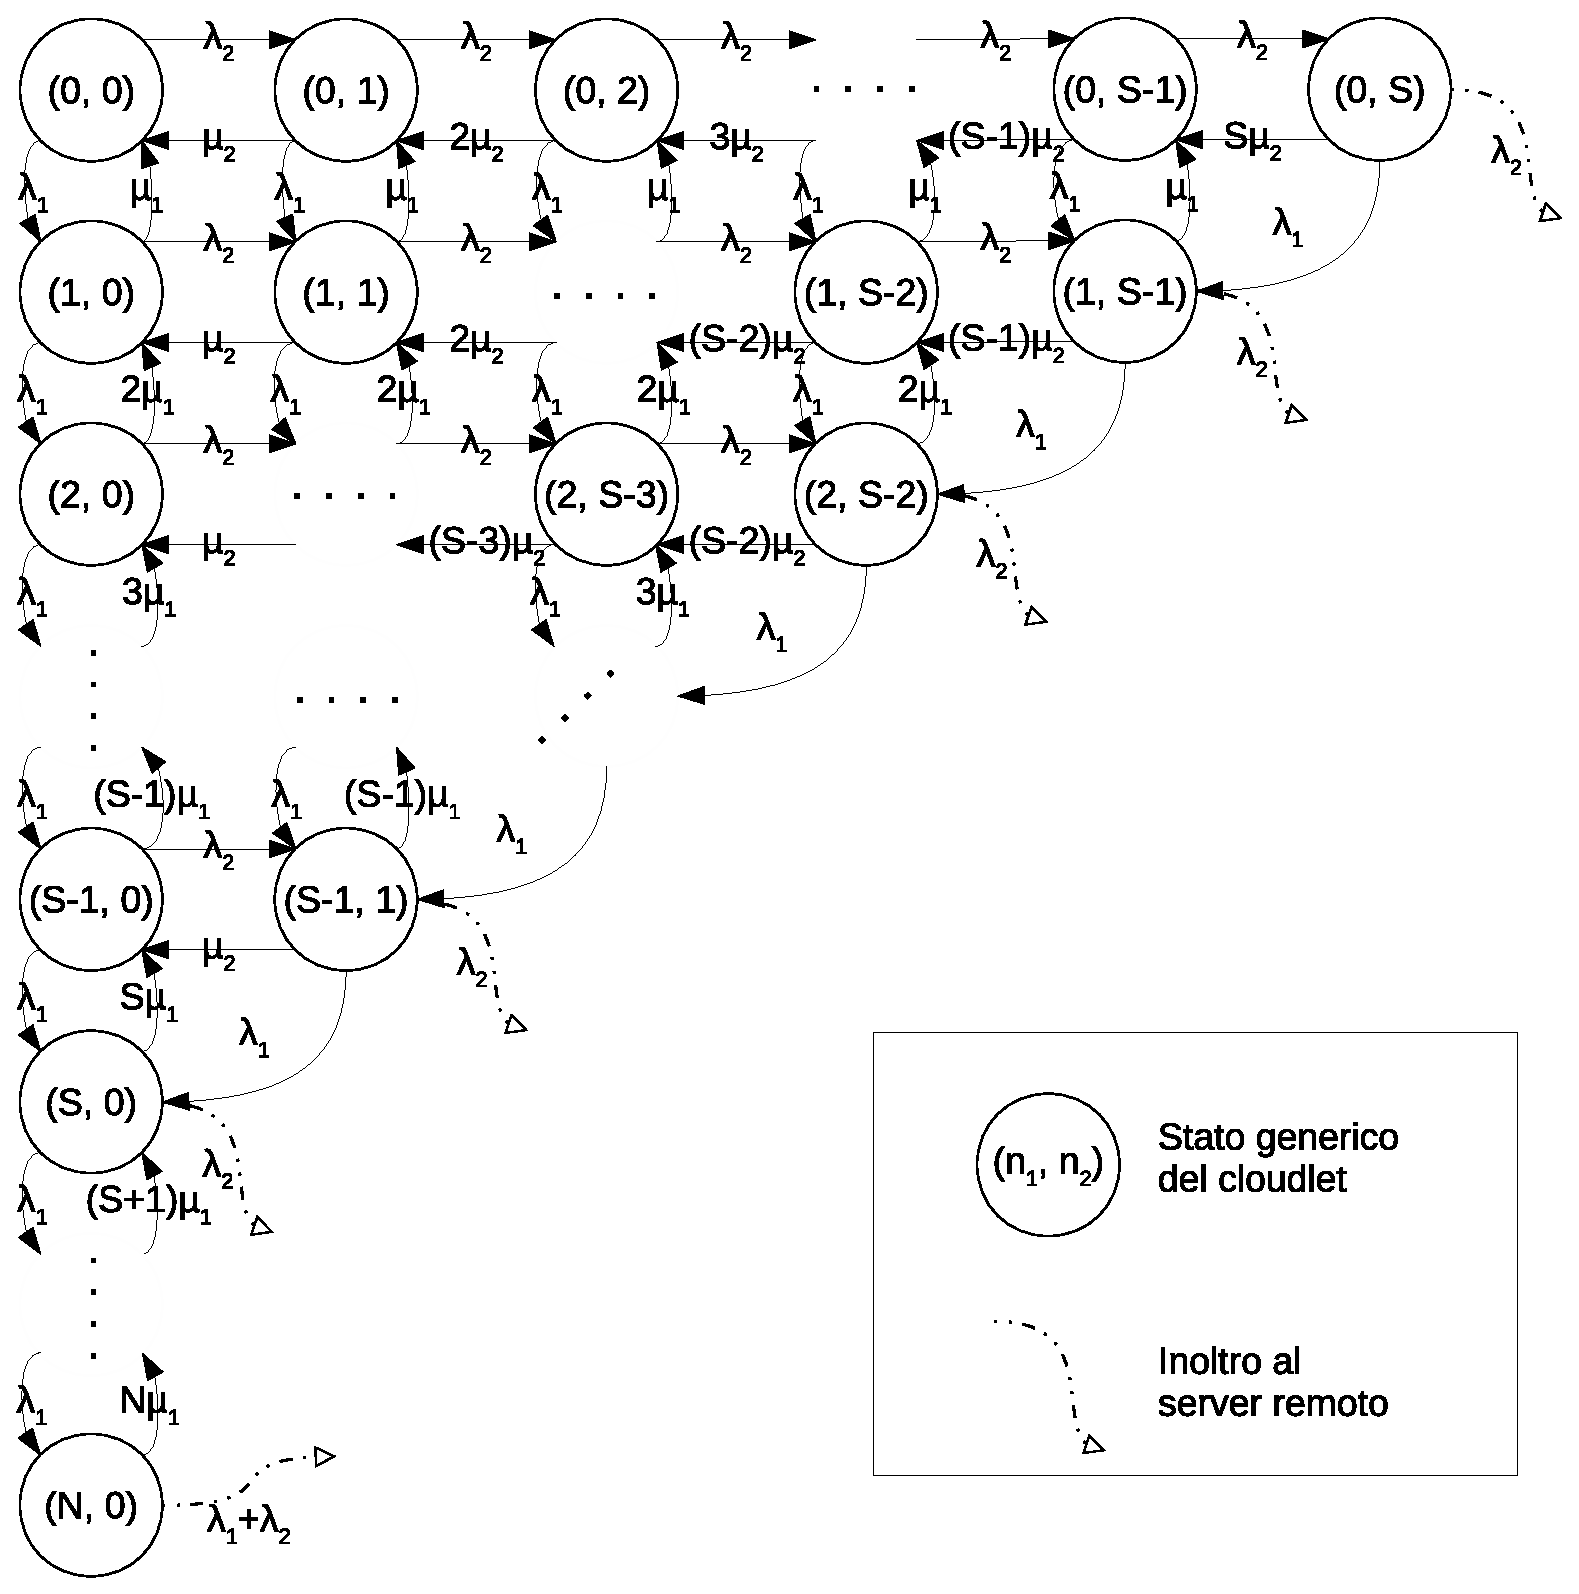
\includegraphics[width=0.7\textwidth]{figures/ctmc}
\caption{CTMC cloudlet}
\label{ctmc}
\end{figure}
%

Per il calcolo della distribuzione stazionaria si è utilizzato un programma di
calcolo basato su matrici scritto in \emph{Matlab}, al fine di risolvere il
seguente sistema di equazioni di bilancio derivanti dall'analisi della catena.
%
\begin{displaymath}
\left\{ \begin{array}{ll}

\lambda \pi_{(0,0)} - \mu_1 \pi_{(1,0)} -\mu_{2} \pi_{(0,1)} = 0 & \\[4pt]

(\lambda+i\mu_1)\pi_{(i,0)} - \lambda_1\pi_{(i-1,0)} + - (i+1)\mu_1\pi_{(i+1,0)}
+ &\\
\qquad - \mu_2\pi_{(i,1)} = 0 & 
\qquad \forall \ i = 1, \ldots, S-1  \\[4pt]  

(\lambda+j\mu_2)\pi_{(0,j)} - \lambda_2\pi_{(0,j-1)} - \mu_1\pi_{(1,j)} + &\\
\qquad-(j+1)\mu_2\pi_{(0,j+1)} = 0 & 
\qquad \forall \ j = 1, \ldots, S-1 \\[4pt]

(\lambda+i\mu_1+j\mu_2)\pi_{(i,j)} - \lambda_1\pi_{(i-1,j)} -
(i+1)\mu_1\pi_{(i+1,j)}+ &\\
\qquad - \lambda_2\pi_{(i,j-1)} -(j+1)\mu_2\pi_{(1,j+1)} = 0 & \qquad \forall \
  i,j=1,\ldots,S-1 : i+j < S \\[4pt]

(\lambda_1+i\mu_1+j\mu_2)\pi_{(i,j)} - \lambda_1(\pi_{(i-1,j)}+\pi_{(i-1,j+1)})
+ &\\
\qquad - \lambda_2\pi_{(i,j-1)} = 0 & 
\qquad \forall \ i,j=1,\ldots,S-1 : i+j = S \\[4pt]

(\lambda_1+S\mu_2)\pi_{(0,S)} - \lambda_2\pi_{(0,S-1)} = 0 & \\[4pt]

(\lambda_1+S\mu_1)\pi_{(S,0)} - \lambda_1(\pi_{(S-1,0)}+\pi_{(S-1,1)}) + &\\
\qquad -(S+1)\mu_1\pi_{(S+1,0)} = 0 & \\[4pt]

(\lambda_1+i\mu_1)\pi_{(i,0)} - \lambda_1\pi_{(i-1,0)} - (i+1)\mu_1\pi_{(i+1,0)}
= 0 & \qquad \forall \ i = S+1,\ldots,N-1 \\[4pt]

\sum_{(i,j) \in E} \pi_{(i,j)} = 1 & 

\end{array} \right .
\end{displaymath}

Si è quindi giunti ad ottenere le probabilità $\pi_{(n_1,n_2)}$ di trovarsi
nello stato $(n_1, n_2) \in E$ in condizioni di stazionarietà, dove E è
l'insieme dei possibili stati della catena.

A questo punto è possibile, sommando le opportune $\pi_{(n_1,n_2)}$, ricondursi
alle probabilità che si verifichino determinati eventi che consentiranno di
stimare le metriche di interesse.
%%
%%
%%
\subsection{Probabilità preliminari}
Prima di tutto è conveniente sfruttare la distribuzione stazionaria per il
calcolo di alcune probabilità preliminari, utili al calcolo dei tempi di
risposta.
\begin{itemize}
\item \emph{Probabilità di Accettazione}: probabilità che il sistema si trovi in
uno stato in cui qualunque job viene accettato in esecuzione nel cloudlet
\begin{equation}
\Pi_A = \sum_{\substack{n_1,n_2:\\n_1 + n_2 < S}} \pi_{(n_1,n_2)}
\end{equation}
\item \emph{Probabilità di Soglia}: probabilità che il sistema si trovi in uno
stato in cui il valore di soglia è stato raggiunto
\begin{equation}
\Pi_S = \sum_{\substack{n_1,n_2:\\ n_1 + n_2 \geq S}} \pi_{(n_1,n_2)}
\end{equation}
\item \emph{Probabilità di Blocco}: probabilità che il sistema si trovi in uno
stato in cui qualunque job viene direttamente inoltrato al server remoto (cloud)
\begin{equation}
\Pi_B = \sum_{\substack{n_1,n_2:\\n_1 + n_2 = N}} \pi_{(n_1,n_2)}
\end{equation}
\item \emph{Probabilità di Interruzione}: probabilità che il sistema si trovi in
uno stato in cui è possibili che un job venga interrotto
\begin{equation}
\Pi_I = \sum_{\substack{n_1,n_2:\\n_1 + n_2 = N\\n_2 > 0}} \pi_{(n_1,n_2)}
\end{equation}
\item \emph{Probabilità di Interruzione a seguito di Accettazione}: probabilità
che un job accettato nel cloudlet venga interrotto, calcolata rapportando la
frequenza di interruzione di un job alla frequenza di accettazione
\begin{equation}
P_{intr}^{clet} = \frac{\lambda_1 \ \Pi_I}{\lambda_2 \ \Pi_A}
\end{equation}
\item \emph{Probabilità di Interruzione di un job di classe 2}: probabilità
che un job di classe 2 venga interrotto, ovvero che venga accettato nel cloudlet
e interrotto
\begin{equation}
P_{intr} = \Pi_A \ P_{intr}^{clet}
\end{equation}
\end{itemize}
%%
%%
%%
\subsection{Stabilità}
Osservando il sistema, si nota che, grazie al server remoto, nel complesso è
composto da un numero di risorse infinito, pertanto è possibile concludere che
l'utilizzazione totale $\rho$ sarà sempre inferiore a $1$ e di conseguenza il
throughput del sistema sarà uguale al tasso di arrivo ($X=\lambda$), ovvero si
può ipotizzare che il sistema sia stabile.

Sotto tale ipotesi è lecito ricorrere alla legge di Little, applicabile
al sistema nel complesso e a tutti i nodi con risorse infinite, purtroppo il
cloudlet non ha tale disponibilità.
%%
%%
%%
\subsection{Throughput}
Per il calcolo del throughput si può sfruttare quindi la condizione di stabilità
del sistema e dei suoi nodi, e poi calcolare il throughput del cloudlet
sottraendo dal throughput del sistema quello del cloud, poiché le uscite dal
nodo di setup non corrispondono a quelle del sistema.

Prima di ciò, però, è necessario ottenere i tassi di arrivo ai singoli nodi e
ciò è possibile considerando i tassi di scarto del cloudlet:
\begin{itemize}
\item[-]I job di classe 1 vengono scartati soltanto nel caso in cui il cloudlet
si trova nello stato $(N, 0)$, ovvero quando vi sono esattamente N job di classe
1 in esecuzione.
\item[-]I job di classe 2 vengono scartati nel caso in cui il cloudlet si trova
in uno stato in cui si è raggiunto il valore di soglia, oppure nel caso in cui
avvenga una sostituzione con uno di classe 1. 
\end{itemize}

In conlusione si ottiene:
\begin{displaymath}
\lambda_1^{cloud} = \Pi_B \ \lambda_1 
\qquad\quad\qquad
\lambda_2^{cloud} = \lambda_{setup} = (\Pi_S + P_{intr}) \ \lambda_2 
\end{displaymath}
%
\begin{eqnarray}
X_j^{cloud} &=& \lambda_j^{cloud}   \qquad\quad\qquad\quad j=1,2 \\
X_{cloud} &=& \lambda_1^{cloud} + \lambda_2^{cloud}   \\
X^{setup} &=& \lambda_{setup}   \\
X_j &=& \lambda_j  \ \quad\qquad\quad\qquad \ \quad j=1,2 \\
X &=& \lambda \\
X_j^{clet} &=& X_j - X_j^{cloud} \ \qquad\quad j=1,2 \\
X_{clet} &=& X - X_{cloud} 
\end{eqnarray}
%%
%%
\subsection{Tempo di risposta: Cloud}
I tempi di risposta specifici per classe sono molto semplici da stimare, e sono
pari al reciproco del rispettivo tasso di servizio:
\begin{eqnarray}
E[S_1^{cloud}] &=& \frac{1}{\mu_1^{cloud}} \\
E[S_2^{cloud}] &=& \frac{1}{\mu_2^{cloud}}
\end{eqnarray}

Il tempo di risposta globale per il cloud è calcolato come una media pesata sul
tipo di job che attraversano il nodo. Nello specifico si ha che una porzione
pari a $\lambda_1^{cloud}/(\lambda_1^{cloud}+\lambda_2^{cloud})$ degli arrivi
totali al cloudlet è di classe 1 e sarà in servizio per un tempo mediamente pari
a $E[S_1^{cloud}]$, la restante porzione
($\lambda_2^{cloud}/(\lambda_1^{cloud}+\lambda_2^{cloud})$) invece è di classe 2
e sarà in servizio per un tempo mediamente pari a $E[S_2^{cloud}]$.

Si ottiene quindi la formula seguente:
\begin{equation}
E[S_{cloud}] = 
\frac{\lambda_1^{cloud}}{\lambda_1^{cloud}+\lambda_2^{cloud}} \ E[S_1^{cloud}] +
\frac{\lambda_2^{cloud}}{\lambda_1^{cloud}+\lambda_2^{cloud}} \ E[S_2^{cloud}] 
\end{equation}
%
\subsection{Tempo di risposta: Cloudlet}
Il tempo medio di risposta di un job di classe 1 per il cloudlet è banalmente il
reciproco del tasso di servizio relativo:
\begin{equation}
E[S_1^{clet}] = \frac{1}{\mu_1^{clet}}
\end{equation}
tale valore è indipendente dal paremtro $S$ ed equivale a $2.\overline2$, mentre
per quanto riguarda i job di classe 2, il tempo medio di servizio subisce una
riduzione dovuta alle interruzioni. Infatti, poiché i job che hanno un tempo
di servizio maggiore del valor medio ($1/\mu_2^{clet}$) permangono nel nodo per
più tempo, sono più soggetti alle interruzioni, quindi
non verranno inclusi nel calcolo del tempo medio ed incideranno maggiormente i
job con un tempo di servizio minore.
Si può stimare che, tale tempo di risposta medio, viene abbattuto di un fattore
$E[S_r]$ proporzionale alla probabilità che un job venga interrotto.
\begin{eqnarray}
E[S_r] &=& \frac{1}{\mu_2^{clet}} \ P_{intr}^{clet}  \nonumber \\
E[S_2^{clet}] &=& \frac{1}{\mu_2^{clet}} - E[S_r]
\end{eqnarray}

Tale stima è ragionevole, poiché se si ragiona al limite si ha che, in assenza
di interruzioni, il tempo di risposta assume il valore normale $1/\mu_2^{clet}$,
altrimenti, con una probabilità di interruzione pari a 1, assume giustamente il
valore nullo, poiché non ci sarebbero completamenti in tali condizioni.
\begin{eqnarray*}
P_{intr}^{clet} \longrightarrow 0 \qquad & \Rightarrow \qquad & 
E[S_r] \rightarrow 0 \ ; \qquad E[S_2^{clet}] \rightarrow
\frac{1}{\mu_2^{clet}} \ \\
P_{intr}^{clet} \longrightarrow 1 \qquad & \Rightarrow \qquad & 
E[S_r] \rightarrow \frac{1}{\mu_2^{clet}} \ ; \qquad E[S_2^{clet}] \rightarrow 0
\end{eqnarray*}

Il tempo di risposta medio globale per il cloudlet non può essere calcolato
considerando la distribuzione degli arrivi nel nodo, perché esiste la
possibilità che arrivi di classe 2 vengano interrotti e quindi che non
contribuiscano al calcolo stesso. Per questo motivo si è considerato il tasso di
uscita: una porzione pari a $X_1^{clet}/(X_1^{clet}+X_2^{clet})$ dei
completaenti totali del cloudlet è di classe 1 e sarà stata in servizio per un
tempo mediamente pari a $E[S_1^{clet}]$, la restante porzione
($X_2^{clet}/(X_1^{clet}+X_2^{clet})$) invece è di classe 2 e sarà stata in
servizio per un tempo mediamente pari a $E[S_2^{clet}]$.  Si ottiene quindi la
formula seguente:
\begin{equation}
E[S_{clet}] = 
\frac{X_1^{clet}}{X_1^{clet}+X_2^{clet}} \ E[S_1^{clet}] +
\frac{X_2^{clet}}{X_1^{clet}+X_2^{clet}} \ E[S_2^{clet}] 
\end{equation}
%
\subsection{Tempo di risposta: Sistema}
Un job di classe 1, al suo arrivo nel sistema, può essere soggetto a due
alternative: essere inoltrato nel cloud nel caso in cui il cloudlet sia saturo
con probabilità $\Pi_B$, oppure essere eseguito nel cloudlet con probabilità
$1-\Pi_B$.
\begin{equation}
E[S_1] = (1-\Pi_B) \ E[S_1^{clet}] \ + \ \Pi_B \ E[S_1^{cloud}]
\end{equation}

Prima di calcolare il tempo di risposta medio dei job di classe 2, è necessario
calcolare il tempo di risposta medio di un job interrotto.\\
Tale tempo è composto dalla somma di tre componenti, partendo dall'ultima: il
tempo medio di servizio nel nodo cloud pari a $E[S_{cloud}]$, il tempo medio di
setup pari a $E[S_{setup}]$ ed infine il tempo medio di esecuzione nel cloudlet
prima che il job venga interrotto.

La stima di quest'ultimo può essere effettuata similmente a quella del calcolo
del tempo di risposta dei job di classe 2 nel cloudlet. Infatti anche in questo
caso è necessario sottrarre un certa quantità al tempo che normalmente avrebbe
impiegato in esecuzione se non ci fosse stata interruzione, ovvero
$1/\mu_2^{clet}$. Sarebbe quindi ideale la relazione del tipo:
\begin{displaymath}
E[Y] = \frac{1}{\mu_2^{clet}}(1 - \beta \ P_{intr}^{clet})
\qquad\quad\qquad 0 < \beta \leq 1
\end{displaymath}
perché si vuole che il tempo di esecuzione antecedente all'interruzione (qui
indicato per semplicità con $Y$) diminuisca all'aumentare della probabilità di
interruzione. Si noti che per $\beta = 1$ si ottiene esattamente la formula di
$E[S_2^{clet}]$, in questo caso però, non si vuole che il tempo di esecuzione
tenda a 0 se la probabilità di interruzione fosse pari a 1, perché tale
situazione non sarebbe realistica, infatti anche se ogni singolo job deve essere
interrotto non si può pensare che esso abbia un tempo di esecuzione nel cloudlet
pari a 0. Per questo motivo, $\beta$ funge da fattore di attenuazione che riduce
l'incisività della probabilità di interruzione sul calcolo.

Tramite il confronto congiunto con le varie simulazioni al variare del parametro
$S$, è stato scelto il un valore del fattore $\beta$ pari a $0.95$. Si è giunti
quindi alla formula seguente per il calcolo del tempo medio di servizio di un
job interrotto:
\begin{equation}
E[S_{intr}] = 
(1 - \beta P_{intr}^{clet}) \frac{1}{\mu_2^{clet}} + E[S_{setup}] + E[S_{cloud}]
\qquad\quad \beta = 0.95
\end{equation}

Un job di classe 2 invece può avere tre diversi tempi di esecuzione in base ai
seguenti casi:
\begin{itemize}
\item[-]Il job viene inoltrato direttamente al cloud remoto perché si è
raggiunto il valore di soglia, dove viene eseguito per un tempo mediamente pari
a $E[S_2^{cloud}]$, questo avviene con probabilità $\Pi_S$;
\item[-]Il job viene accettato nel cloudlet e non viene interrotto, il suo tempo
di esecuzione è mediamente pari a $E[S_2^{clet}]$, questo accade con probabilità
$\Pi_A (1 - P_{intr}^{clet})$;
\item[-]Il job viene eseguito nel cloudlet, viene interrotto ed inoltrato al
server remoto in cui viene eseguito dopo una fase di setup, questo avviene con
probabilità $P_{intr}$ ed il tempo di esecuzione è mediamente pari a 
$E[S_{intr}]$; 
\end{itemize}
Pertanto un job di classe 2 ha un tempo di risposta medio che deriva dalla
seguente formula:
\begin{equation}
E[S_2] \ = \
\Pi_S E[S_2^{cloud}] \ + \ \Pi_A (1-P_{intr}^{clet}) E[S_2^{clet}] \ + \ 
P_{intr} E[S_{intr}]
\end{equation}
Il tempo di risposta globale del sistema è calcolato analogamente al caso del
cloud, con i tempi di servizio riferiti al sistema intero, si ha quindi:
\begin{equation}
E[S] \ = \
\frac{\lambda_1}{\lambda_1+\lambda_2}  E[S_1] \ + \
\frac{\lambda_2}{\lambda_1+\lambda_2}  E[S_2] 
\end{equation}
%
%
\subsection{Popolazione media: Cloud}
Per il calcolo della popolazione media del cloud si può sfruttare l'ipotesi di
stabilità e applicare la legge di Little:
\begin{eqnarray}
E[N_j^{cloud}] &=& \lambda_j^{cloud} E[S_j^{cloud}]  \qquad\quad\qquad j=1,2 \\
E[N_{cloud}] &=& (\lambda_1^{cloud} + \lambda_2^{cloud}) E[S_{cloud}]
\end{eqnarray}
%
\subsection{Popolazione media: Cloudlet}
La popolazione media del cloudlet, sia per classe che globale, viene calcolata
sommando il prodotto, relativo ad ogni stato, tra il numero di job presenti in
esso per la probabilità di trovarcisi in condizioni di stazionarietà, ovvero:
\begin{eqnarray}
E[N_1^{clet}] &=& \sum_{(n_1,n_2) \in E} n_1 \ \pi_{(n_1,n_2)} \\
E[N_2^{clet}] &=& \sum_{(n_1,n_2) \in E} n_2 \ \pi_{(n_1,n_2)} \\
E[N_{clet}] &=& \sum_{(n_1,n_2) \in E} (n_1+n_2) \ \pi_{(n_1,n_2)} 
\end{eqnarray}
%
\subsection{Popolazione media: Setup}
Anche il nodo di setup può essere considerato stabile.
Si può applicare la legge di Little con un tasso di arrivi a questo nodo pari al
tasso di interruzione dei job di classe 2.
\begin{equation}
E[N^{cloud}] = \lambda_{setup} \ E[S_{setup}] 
\end{equation}
%
\subsection{Popolazione media: Sistema}
Sempre sfruttando l'ipotesi di stabilità si ottiene:
\begin{eqnarray}
E[N_j] &=& \lambda_j E[S_j]  \qquad\quad\qquad j=1,2 \\
E[N] &=& (\lambda_1 + \lambda_2) E[S]
\end{eqnarray}
%

\section{Risultati}
\newcommand{\epsmx}{$\varepsilon_{max}$}
La validazione dei modelli appena discussi è stata effettuata confrontando i
risultati della simulazione con le stime dedotte dall'analisi, valutando quattro
possibili scenari contraddistinti dal valore che assume il parametro $S$.

Ognuno di questi scenari è stato simulato facendo processare al programma lo
stesso numero di job affinché le statistiche globali del sistema potessero 
essere confrontate. Tale numero è stato stabilito in base alle metriche che
andavano valutate ed al numero di job che le riguardava.

Lo scenario con valore di soglia $S=5$, è quello in cui soltanto circa il $2\%$
dei job di classe 2 è processato nel cloudlet e di questi circa il $90\%$
vengono interrotti, ne risulta quindi che, in relazione al numero totale dei job
che transitano nel sistema, solamente lo $0.14\%$ sono job di classe 2
processati con successo nel cloudlet e l'$1.37\%$ sono job interrotti. In
definitiva, al fine di avere una dimensione dei batch soddisfacente per il
calcolo delle relative metriche, è stato scelto un numero totale di job pari a
$500000$. In questo modo si ottiene un numero di job di classe 2 processati con
successo nel cloudlet pari a circa $700$ e un numero di job interrotti pari a
circa $6850$, ciò significa che per un valore $k=64$ corrispondente al numero
di batch, si ottengono batch di dimensione $10$ e $107$ rispettivamente, che
sono sufficienti a determinare intervalli di confidenza, seppur con un ampio
margine di errore.

Quello appena descritto è il peggior scenario possibile, in cui si registra il
minor numero di job per una determinata metrica, gli altri scenari vengono
quindi simulati tutti con un numero totale di job pari a $500000$, e a seconda
del numero di job che verranno processati nei vari nodi e della loro tipologia,
sono risultati intervalli di confidenza più o meno precisi.

Purtroppo è stato impossibile determinare risultati attendibili per i job
di classe 1 che vengono processati nel cloud, poiché il loro numero è, per ogni
scenario, talmente esiguo che per avere un batch di dimensione 10 sarebbero
necessari almeno 3 milioni di job in tutto. Tuttavia, con un numero di
$500000$ job totali, si ottengono delle statistiche globali molto attendibili,
 ad esempio per il tempo medio di risposta del sistema, si ottiene 
una dimensione del batch pari a $\lfloor\frac{500000}{64}\rfloor = 7812$.

Per ogni statistica vengono presentati grafici e tabelle, in cui vengono
confrontati i risulatati osservati in 10 repliche della simulazione con la
relativa stima del modello analitico, inoltre nelle tabelle viene anche indicato
l'errore massimo \epsmx che è stato commesso, corrispondente al massimo delle
distanze tra la stima e l'estremo più lontano di ogni intervallo di confidenza.
%
%
%%%%%%%%%%%%%%%%%%%%%%%%%%%%%%%%%%%%%%%%%%%%%%%%%%%%%%%%%%%%%%%%%%%%%%%%%%%%%%%%
%%%%%%%%%%%%%%%%%%%%%%%%%%%%%%%%%%%%%%%%%%%%%%%%%%%%%%%%%%%%%%%%%%%%%%%%%%%%%%%%
%%%%%%%%%%%%%%%%%%%%%%%%%%%%%%%%%%%%%%%%%%%%%%%%%%%%%%%%%%%%%%%%%%%%%%%%%%%%%%%%
\subsection{Percentuale Interruzioni}
Per comprendere al meglio l'analisi delle simulazioni ed il confronto con le
stime effettuate è conveniente iniziare dalla presentazione dei risultati
riguardanti la percentuale di job di classe 2 interrotti, poiché da questi
dipendono la maggior parte delle metriche successive.

I grafici in figura~\ref{plot:intperc} mostrano che, nei casi in cui
$S=20,15,10$, la stima della percentuale di interruzione risulta leggermente
inferiore dei valori osservati nelle simulazioni e l'errore massimo che viene
commesso è di circa il $5$-$6\%$, mentre per quanto riguarda il caso in cui
$S=5$ si ottiene una stima leggermente migliore, ma ciò è dovuto al basso
valore della soglia che impedisce ai job di classe 2 di accedere al cloudlet, di
conseguenza è stata riscontrata una maggiore variabilità dei valori delle
simulazioni e si commette infatti un'errore massimo più alto pari al $7.6\%$.

La maggiore percentuale di job interrotti (circa del $30\%$ considerando le
varie repliche), si ottiene per $S=10$, mentre nei restanti due casi non si
hanno valori troppo discordanti, differiscono infatti di circa un punto
percentuale.

I valori delle simulazioni e gli errori relativi rispetto alla stima del modello
analitico sono riportati nelle tabella~\ref{tab:intperc}.
%
\begin{figure}[!h]
\centering
%
\begin{subfigure}[t]{0.49\textwidth}
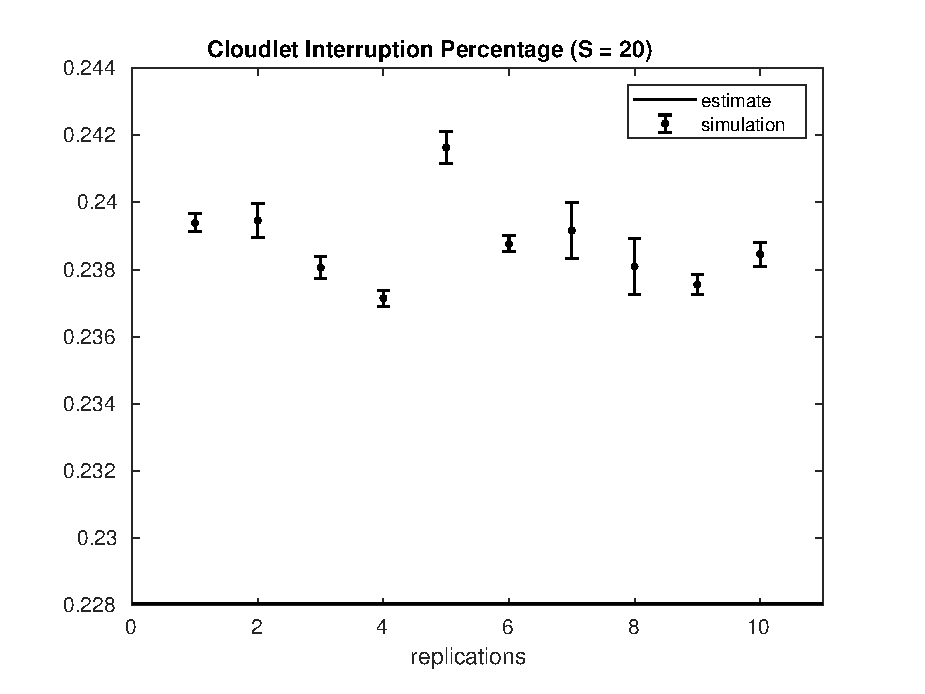
\includegraphics[width=\textwidth]{figures/simul/20_500K_intperc}
\caption{$S = 20$}
\label{20_intperc}
\end{subfigure}
%
\begin{subfigure}[t]{0.49\textwidth}
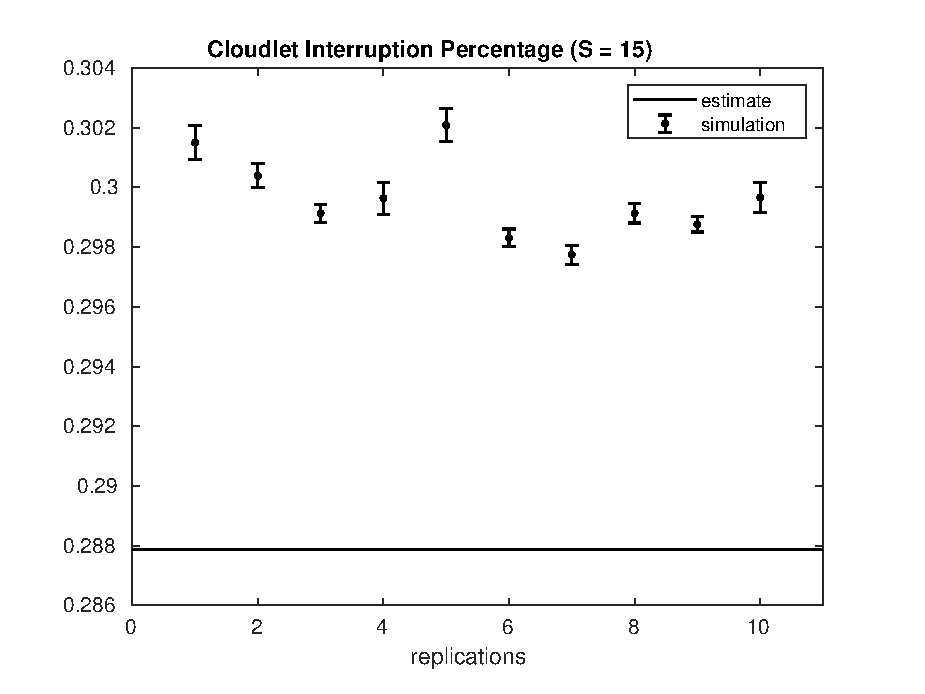
\includegraphics[width=\textwidth]{figures/simul/15_500K_intperc}
\caption{$S = 15$}
\label{15_intperc}
\end{subfigure}
%
\begin{subfigure}[t]{0.49\textwidth}
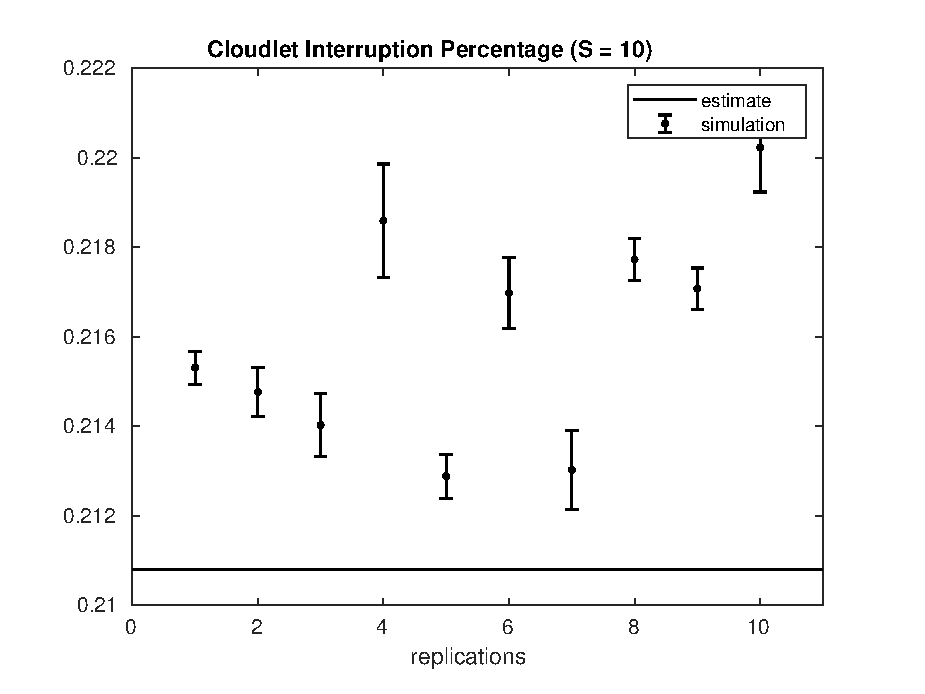
\includegraphics[width=\textwidth]{figures/simul/10_500K_intperc}
\caption{$S = 10$}
\label{10_intperc}
\end{subfigure}
%
\begin{subfigure}[t]{0.49\textwidth}
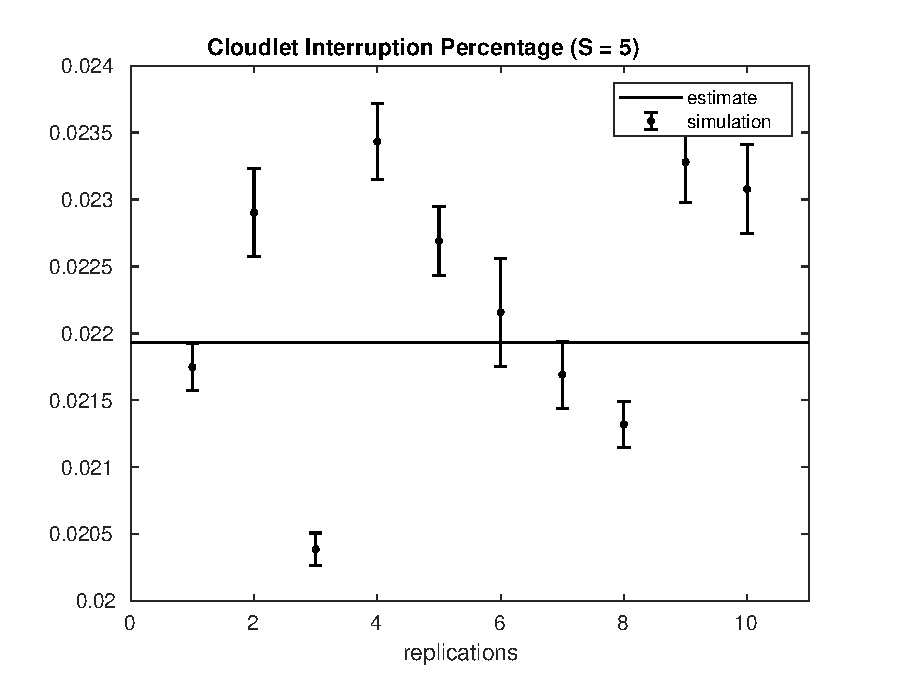
\includegraphics[width=\textwidth]{figures/simul/5_500K_intperc}
\caption{$S = 5$}
\label{5_intperc}
\end{subfigure}
%
\caption{Percentuale di interruzioni}
\label{plot:intperc}
\end{figure}
%
%
\begin{table}[!h]
\begin{adjustbox}{width=\textwidth}
\begin{tabular}{c|r@{.}l|r@{.}l|r@{.}l|r@{.}l}
& \multicolumn{2}{|c|}{$S=20$}
& \multicolumn{2}{|c}{$S=15$}
& \multicolumn{2}{|c}{$S=10$}
& \multicolumn{2}{|c}{$S=5$}
\\          
\hline
R1     & $0$&$2394 \pm 0.0003$ & $0$&$3015 \pm 0.0006$ & $0$&$2153 \pm 0.0004$ & $0$&$0217 \pm 0.0002$ \\
R2     & $0$&$2395 \pm 0.0005$ & $0$&$3004 \pm 0.0004$ & $0$&$2148 \pm 0.0005$ & $0$&$0229 \pm 0.0003$ \\
R3     & $0$&$2381 \pm 0.0003$ & $0$&$2991 \pm 0.0003$ & $0$&$2140 \pm 0.0007$ & $0$&$0204 \pm 0.0001$ \\
R4     & $0$&$2371 \pm 0.0002$ & $0$&$2996 \pm 0.0005$ & $0$&$2186 \pm 0.0013$ & $0$&$0234 \pm 0.0003$ \\
R5     & $0$&$2416 \pm 0.0005$ & $0$&$3021 \pm 0.0006$ & $0$&$2129 \pm 0.0005$ & $0$&$0227 \pm 0.0003$ \\
R6     & $0$&$2388 \pm 0.0002$ & $0$&$2983 \pm 0.0003$ & $0$&$2170 \pm 0.0008$ & $0$&$0222 \pm 0.0004$ \\
R7     & $0$&$2392 \pm 0.0008$ & $0$&$2977 \pm 0.0003$ & $0$&$2130 \pm 0.0009$ & $0$&$0217 \pm 0.0003$ \\
R8     & $0$&$2381 \pm 0.0008$ & $0$&$2991 \pm 0.0003$ & $0$&$2177 \pm 0.0005$ & $0$&$0213 \pm 0.0002$ \\
R9     & $0$&$2376 \pm 0.0003$ & $0$&$2988 \pm 0.0003$ & $0$&$2171 \pm 0.0005$ & $0$&$0233 \pm 0.0003$ \\
R10    & $0$&$2385 \pm 0.0004$ & $0$&$2997 \pm 0.0005$ & $0$&$2202 \pm 0.0010$ & $0$&$0231 \pm 0.0003$ \\
EST    & $0$&$2280$            & $0$&$2879$            & $0$&$2108$            & $0$&$0219$            \\
\epsmx & $0$&$0141 \ (5.8\%)$  & $0$&$0148 \ (4.9\%)$  & $0$&$0104 \ (4.7\%)$  & $0$&$0018 \ (7.6\%)$    
\end{tabular}
\end{adjustbox}
\caption{percentuale job di classe 2 interrotti $S=20$}
\label{tab:intperc}
\end{table}

%%%%%%%%%%%%%%%%%%%%%%%%%%%%%%%%%%%%%%%%%%%%%%%%%%%%%%%%%%%%%%%%%%%%%%%%%%%%%%%%
\subsection{Tempo di Risposta Cloudlet Classe 1}
Il tempo di risposta per un job di classe 1 che viene eseguito nel cloudlet è
indipendente dal parametro S ed i risultati presentati in
figura~\ref{plot:s1clet} e nella tabella~\ref{tab:s1clet} mostrano che tutti gli
intervalli di confidenza calcolati comprendono il valore stimato e in tutti casi
l'errore massimo è sotto la soglia dell'$1\%$.
\begin{figure}[!h]
\centering
%
\begin{subfigure}[t]{0.49\textwidth}
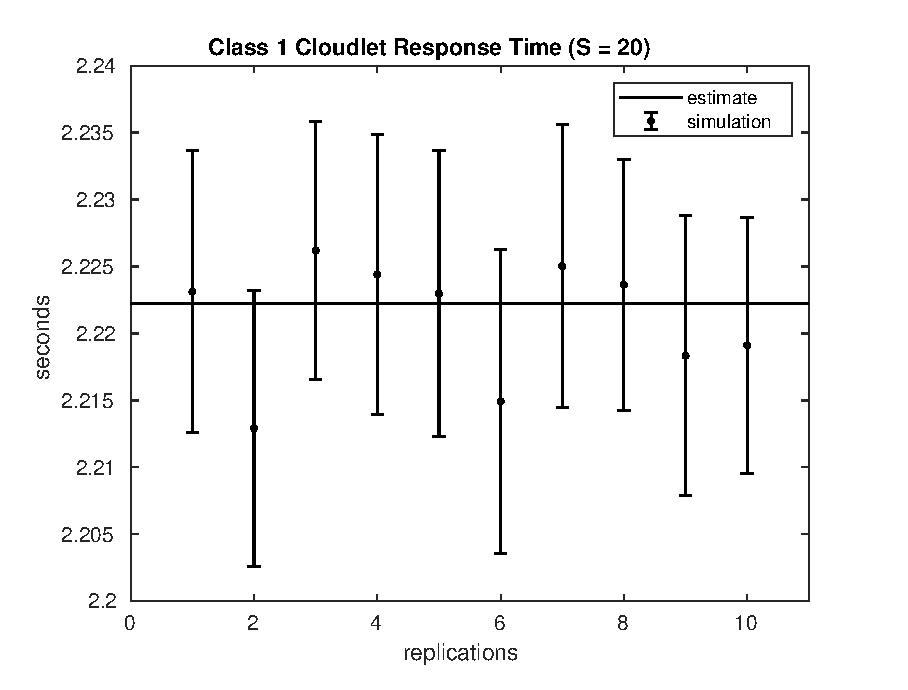
\includegraphics[width=\textwidth]{figures/simul/20_500K_s1clet}
\caption{$S = 20$}
\label{20_s1clet}
\end{subfigure}
%
\begin{subfigure}[t]{0.49\textwidth}
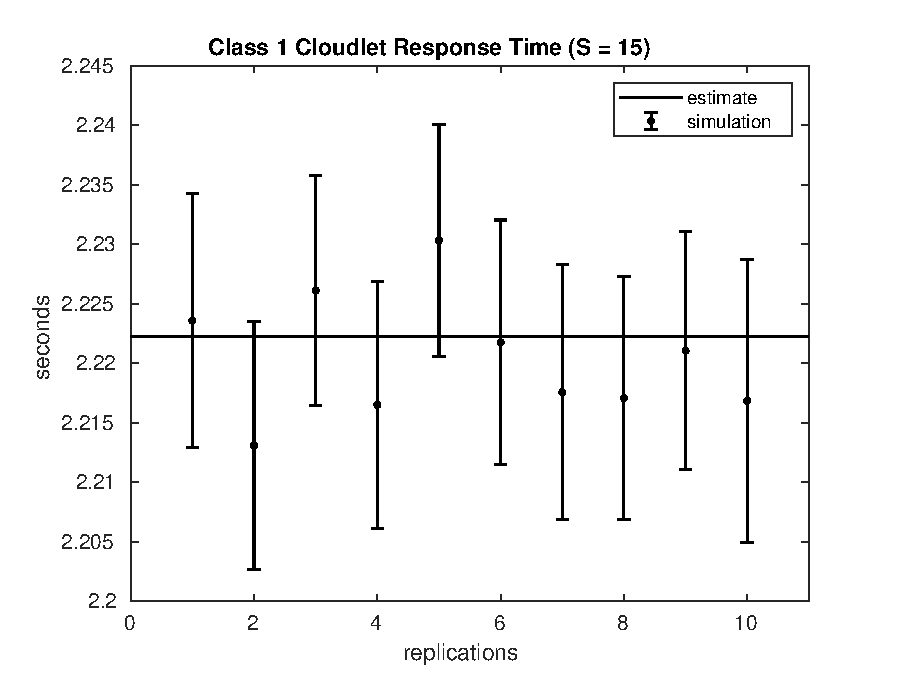
\includegraphics[width=\textwidth]{figures/simul/15_500K_s1clet}
\caption{$S = 15$}
\label{15_s1clet}
\end{subfigure}
%
\begin{subfigure}[t]{0.49\textwidth}
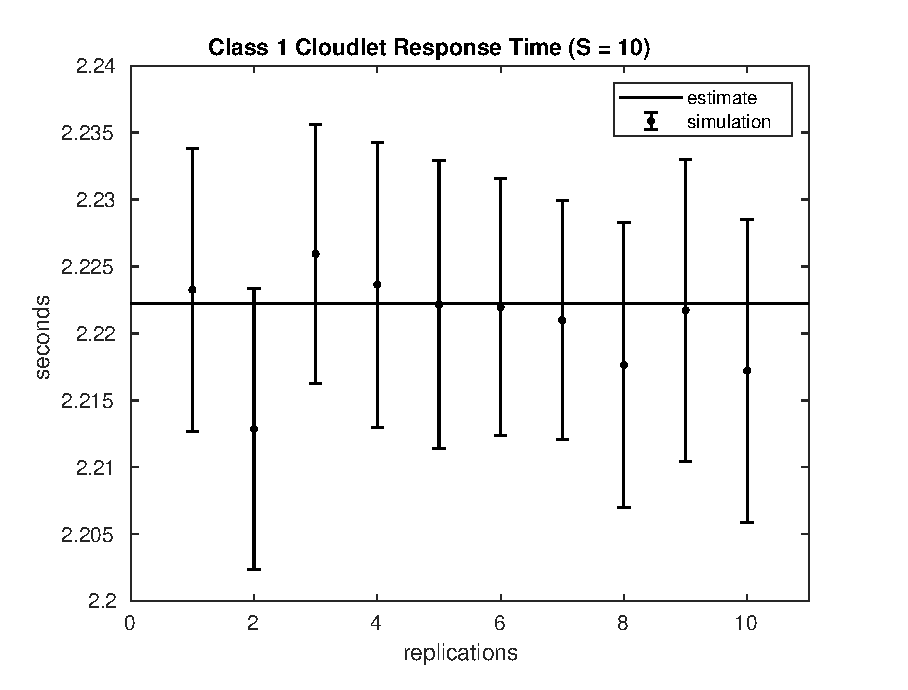
\includegraphics[width=\textwidth]{figures/simul/10_500K_s1clet}
\caption{$S = 10$}
\label{10_s1clet}
\end{subfigure}
%
\begin{subfigure}[t]{0.49\textwidth}
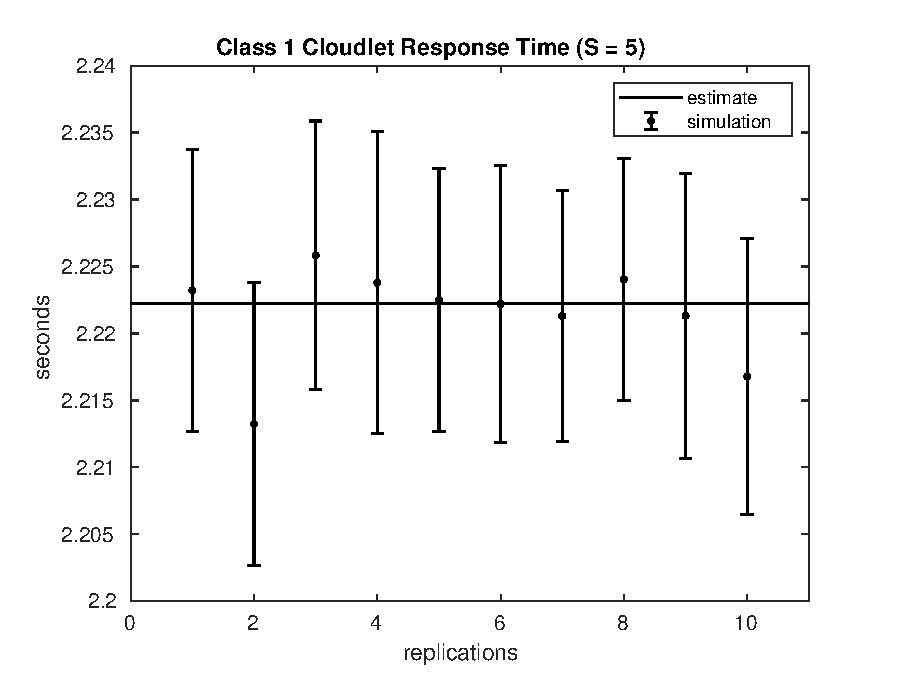
\includegraphics[width=\textwidth]{figures/simul/5_500K_s1clet}
\caption{$S = 5$}
\label{5_s1clet}
\end{subfigure}
%
\caption{tempo di risposta cloudlet classe 1}
\label{plot:s1clet}
\end{figure}
%
%
\begin{table}[!h]
\begin{adjustbox}{width=\textwidth}
\begin{tabular}{c|r@{.}l|r@{.}l|r@{.}l|r@{.}l}
& \multicolumn{2}{|c|}{$S=20$}
& \multicolumn{2}{|c|}{$S=15$}
& \multicolumn{2}{|c|}{$S=10$}
& \multicolumn{2}{|c}{$S=5$}
\\          
\hline
R1      & $2$&$2231 \pm 0.0105$ & $2$&$2236 \pm 0.0107$ & $2$&$2233 \pm 0.0106$ & $2$&$2231 \pm 0.0105$ \\
R2      & $2$&$2129 \pm 0.0103$ & $2$&$2131 \pm 0.0104$ & $2$&$2129 \pm 0.0105$ & $2$&$2129 \pm 0.0103$ \\
R3      & $2$&$2262 \pm 0.0096$ & $2$&$2261 \pm 0.0096$ & $2$&$2259 \pm 0.0097$ & $2$&$2262 \pm 0.0096$ \\
R4      & $2$&$2244 \pm 0.0105$ & $2$&$2165 \pm 0.0104$ & $2$&$2236 \pm 0.0106$ & $2$&$2244 \pm 0.0105$ \\
R5      & $2$&$2230 \pm 0.0107$ & $2$&$2303 \pm 0.0097$ & $2$&$2222 \pm 0.0107$ & $2$&$2230 \pm 0.0107$ \\
R6      & $2$&$2149 \pm 0.0113$ & $2$&$2218 \pm 0.0103$ & $2$&$2220 \pm 0.0096$ & $2$&$2149 \pm 0.0113$ \\
R7      & $2$&$2250 \pm 0.0106$ & $2$&$2176 \pm 0.0107$ & $2$&$2210 \pm 0.0089$ & $2$&$2250 \pm 0.0106$ \\
R8      & $2$&$2236 \pm 0.0094$ & $2$&$2171 \pm 0.0102$ & $2$&$2177 \pm 0.0107$ & $2$&$2236 \pm 0.0094$ \\
R9      & $2$&$2183 \pm 0.0104$ & $2$&$2211 \pm 0.0100$ & $2$&$2217 \pm 0.0113$ & $2$&$2183 \pm 0.0104$ \\
R10     & $2$&$2191 \pm 0.0095$ & $2$&$2168 \pm 0.0119$ & $2$&$2172 \pm 0.0113$ & $2$&$2191 \pm 0.0095$ \\
EST     & $2$&$2222$            & $2$&$2222$            & $2$&$2222$            & $2$&$2222$            \\
\epsmx  & $0$&$0136 \ (0.6\%)$  & $0$&$0178 \ (0.8\%)$  & $0$&$0134 \ (0.6\%)$  & $0$&$0136 \ (0.6\%)$    
\end{tabular}
\end{adjustbox}
\caption{tempo di risposta cloudlet classe 1}
\label{tab:s1clet}
\end{table}

%%%%%%%%%%%%%%%%%%%%%%%%%%%%%%%%%%%%%%%%%%%%%%%%%%%%%%%%%%%%%%%%%%%%%%%%%%%%%%%%
\subsection{Tempo di Risposta Cloudlet Classe 2}
La figura~\ref{plot:s2clet} e la tabella~\ref{tab:s2clet} mostrano un tempo di
risposta medio per i job di classe 2 eseguiti nel cloudlet che cresce/decresce
in modo proporzionale ad $S$, ciò sta a indicare che la probabilità di
interruzione di un job in esecuzione nel cloudlet ($P_{intr}^{clet}$) è
inversamente proporzionale a $S$ ed incide maggiormente nell'abbattimento del
tempo di risposta laddove $S$ è minore.

La stima effettuata, nei casi in cui $S=20,15,10$, è affidabile con un errore
massimo del $5\%$, mentre, nel caso in cui $S=5$, gli intervalli di confidenza
hanno un ampiezza eccessiva con un errore anche del $104\%$, quest'ultimo fatto
è dovuto al basso valore del parametro di soglia che impedisce l'accesso ai job
di classe 2 e all'elevato tasso di interruzione per i pochi che vengono
accettati nel nodo, risulta così un ridotto numero di job di classe 2 che
vengono processati nel cloudlet, e di conseguenza una dimensione dei batch
troppo piccola per ottenere intervalli precisi.
\begin{figure}[!h]
\centering
%
\begin{subfigure}[t]{0.49\textwidth}
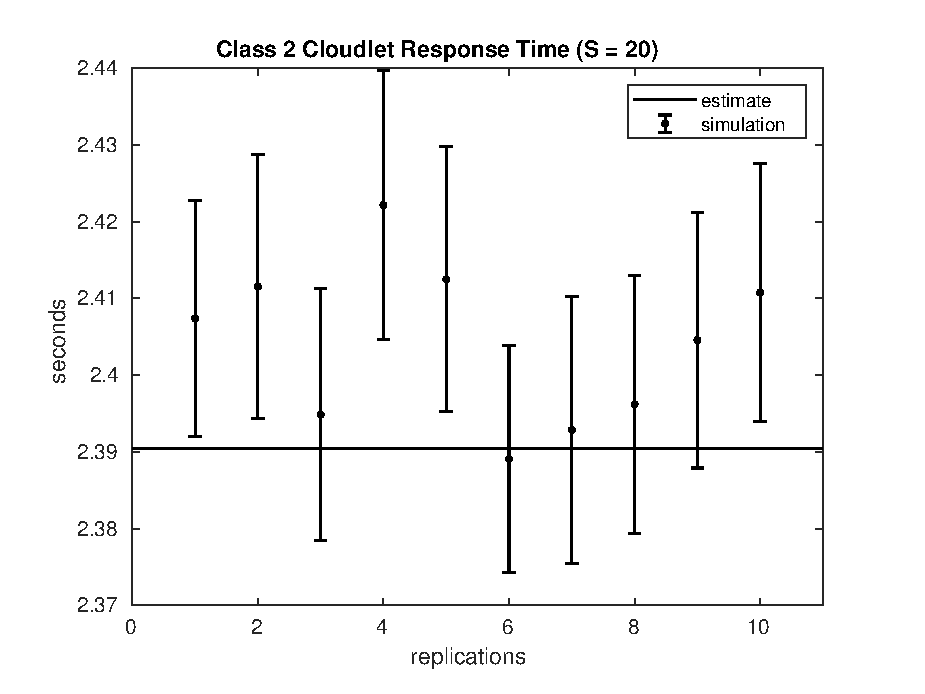
\includegraphics[width=\textwidth]{figures/simul/20_500K_s2clet}
\caption{$S = 20$}
\label{20_s2clet}
\end{subfigure}
%
\begin{subfigure}[t]{0.49\textwidth}
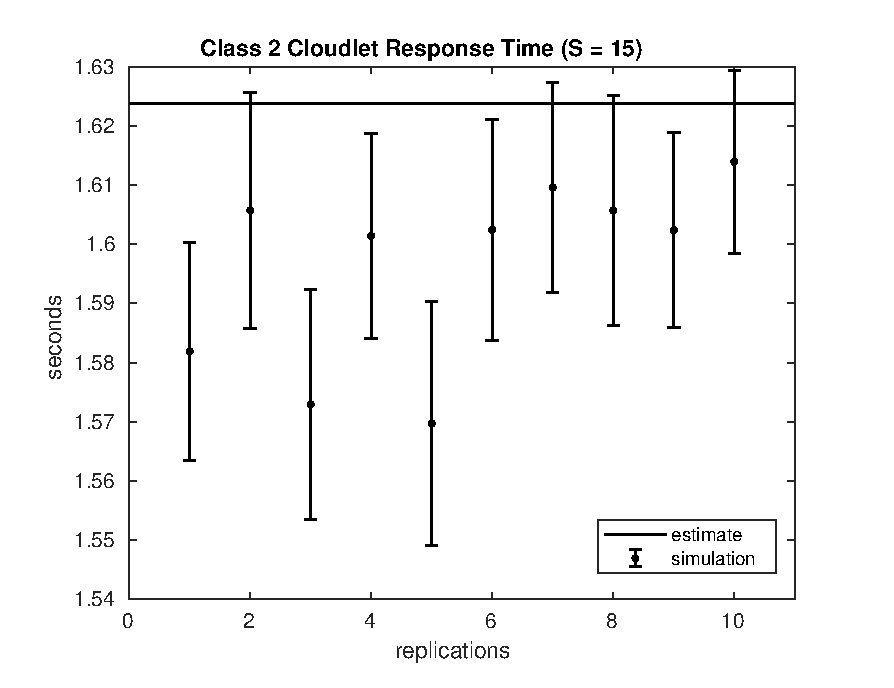
\includegraphics[width=\textwidth]{figures/simul/15_500K_s2clet}
\caption{$S = 15$}
\label{15_s2clet}
\end{subfigure}
%
\begin{subfigure}[t]{0.49\textwidth}
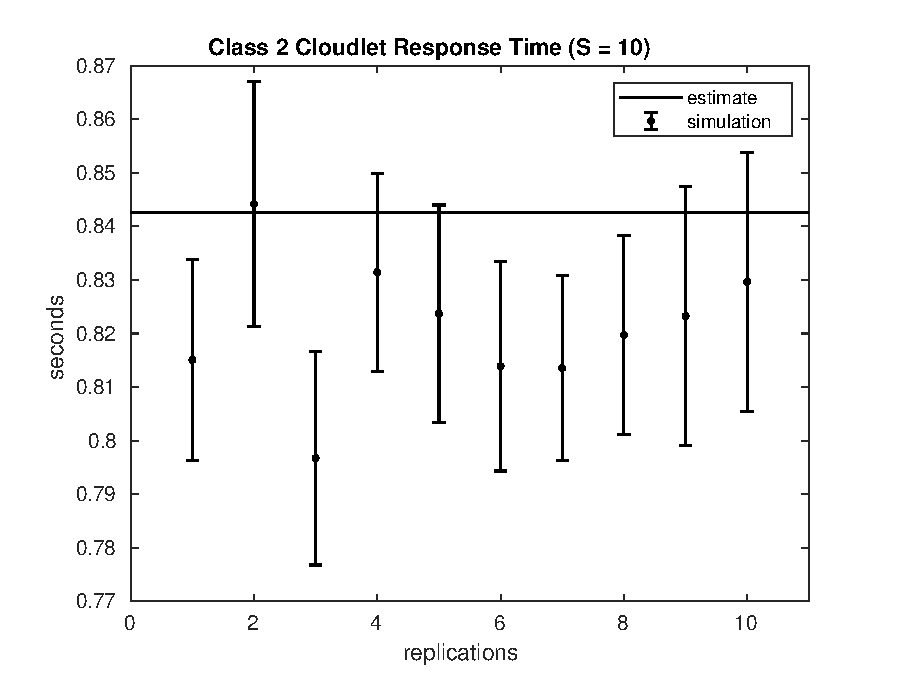
\includegraphics[width=\textwidth]{figures/simul/10_500K_s2clet}
\caption{$S = 10$}
\label{10_s2clet}
\end{subfigure}
%
\begin{subfigure}[t]{0.49\textwidth}
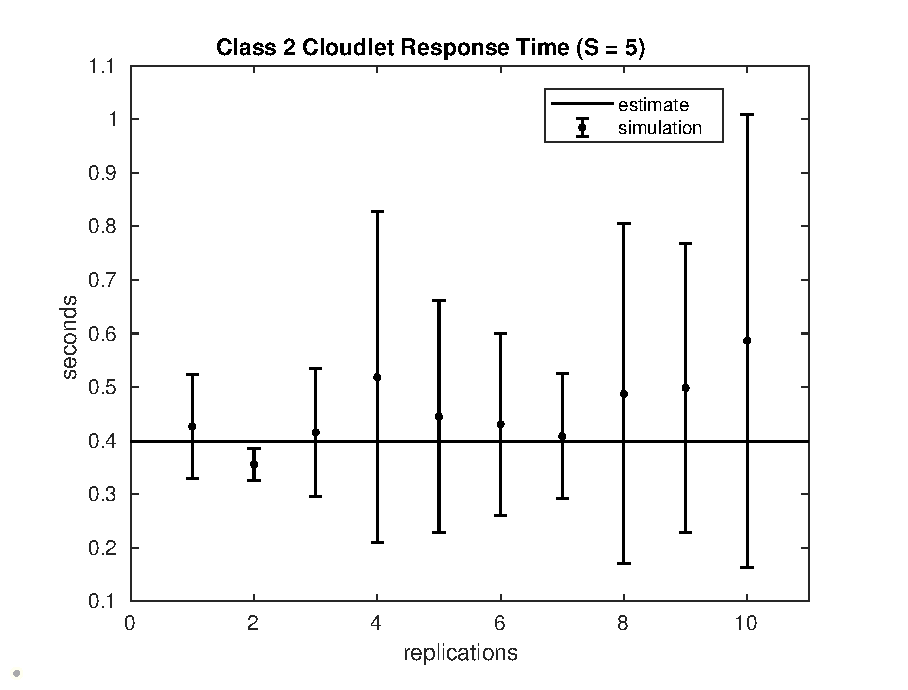
\includegraphics[width=\textwidth]{figures/simul/5_500K_s2clet}
\caption{$S = 5$}
\label{5_s2clet}
\end{subfigure}
%
\caption{tempo di risposta cloudlet classe 2}
\label{plot:s2clet}
\end{figure}
%
%
\begin{table}[!h]
\begin{adjustbox}{width=\textwidth}
\begin{tabular}{c|r@{.}l|r@{.}l|r@{.}l|r@{.}l}
& \multicolumn{2}{|c|}{$S=20$}
& \multicolumn{2}{|c|}{$S=15$}
& \multicolumn{2}{|c|}{$S=10$}
& \multicolumn{2}{|c}{$S=5$}
\\          
\hline
R1      & $2$&$4074 \pm 0.0153$ & $1$&$5819 \pm 0.0184$ & $0$&$8151 \pm 0.0187$ & $0$&$4265 \pm 0.0976$  \\
R2      & $2$&$4115 \pm 0.0172$ & $1$&$6057 \pm 0.0200$ & $0$&$8441 \pm 0.0228$ & $0$&$3558 \pm 0.0302$  \\
R3      & $2$&$3949 \pm 0.0164$ & $1$&$5730 \pm 0.0195$ & $0$&$7968 \pm 0.0199$ & $0$&$4156 \pm 0.1189$  \\
R4      & $2$&$4221 \pm 0.0175$ & $1$&$6014 \pm 0.0173$ & $0$&$8314 \pm 0.0185$ & $0$&$5185 \pm 0.3093$  \\
R5      & $2$&$4125 \pm 0.0172$ & $1$&$5697 \pm 0.0206$ & $0$&$8237 \pm 0.0203$ & $0$&$4449 \pm 0.2161$  \\
R6      & $2$&$3891 \pm 0.0148$ & $1$&$6024 \pm 0.0186$ & $0$&$8139 \pm 0.0196$ & $0$&$4307 \pm 0.1697$  \\
R7      & $2$&$3929 \pm 0.0173$ & $1$&$6096 \pm 0.0178$ & $0$&$8136 \pm 0.0173$ & $0$&$4085 \pm 0.1162$  \\
R8      & $2$&$3962 \pm 0.0168$ & $1$&$6057 \pm 0.0194$ & $0$&$8197 \pm 0.0186$ & $0$&$4874 \pm 0.3175$  \\
R9      & $2$&$4046 \pm 0.0167$ & $1$&$6024 \pm 0.0165$ & $0$&$8232 \pm 0.0241$ & $0$&$4984 \pm 0.2696$  \\
R10     & $2$&$4107 \pm 0.0168$ & $1$&$6139 \pm 0.0155$ & $0$&$8296 \pm 0.0242$ & $0$&$5865 \pm 0.4225$  \\
EST     & $2$&$3904$            & $1$&$6238$            & $0$&$8425$            & $0$&$3980$             \\
\epsmx  & $0$&$0492 \ (2.0\%)$  & $0$&$0336 \ (2.1\%)$  & $0$&$0258 \ (3.2\%)$  & $0$&$6110 \ (104.2\%)$   
\end{tabular}
\end{adjustbox}
\caption{tempo di risposta cloudlet classe 2}
\label{tab:s2clet}
\end{table}

%%%%%%%%%%%%%%%%%%%%%%%%%%%%%%%%%%%%%%%%%%%%%%%%%%%%%%%%%%%%%%%%%%%%%%%%%%%%%%%%%
\subsection{Tempo di Risposta Cloudlet}
I risultati della simulazione (figura~\ref{plot:sclet} e
tabella~\ref{tab:sclet}) mostrano come il clodlet reagisce in base ai diversi
scenari:
\begin{itemize}
\item[$S=5$ :] l'esiguo numero di job di classe 2 processati nel cloudlet
discusso in precedenza, fa sì che nel cloudlet è come se fossero eseguiti
soltanto job di classe 1, infatti il tempo di risposta medio globale del nodo è
molto vicino al tempo di risposta medio di quest'ultimi;
\item[$S=20$ :] in questo caso le interruzioni comportano una riduzione
significativa del tempo di servizio medio dei job di classe 2, pertanto il tempo
di risposta medio globale del cloudlet ne risulta attenuato;
\item[$S=10,15$ :] il maggior numero di interruzioni riduce di molto il tempo di
servizio medio dei job di classe 2, in maniera tale da portare il tempo di
risposta medio globale del cloudlet al di sotto del tempo che si avrebbe nel
caso in cui fossero eseguiti soltanto job di classe 1.
\end{itemize}

Le stime effettuate si avvicinano ai valori delle simulazioni con un errore che
va dallo $0.7\%$ del caso in cui $S=10$ all' $1.7\%$ del caso in cui $S=5$.
Degno di nota è il fatto che, in quest'ultimo caso, l'errore sulla stima della
statistica di classe 2 precedente non ha inciso particolarmente, sempre
per via dell'esiguo numero di job processati della suddetta classe.
\begin{figure}[!h]
\centering
%
\begin{subfigure}[t]{0.49\textwidth}
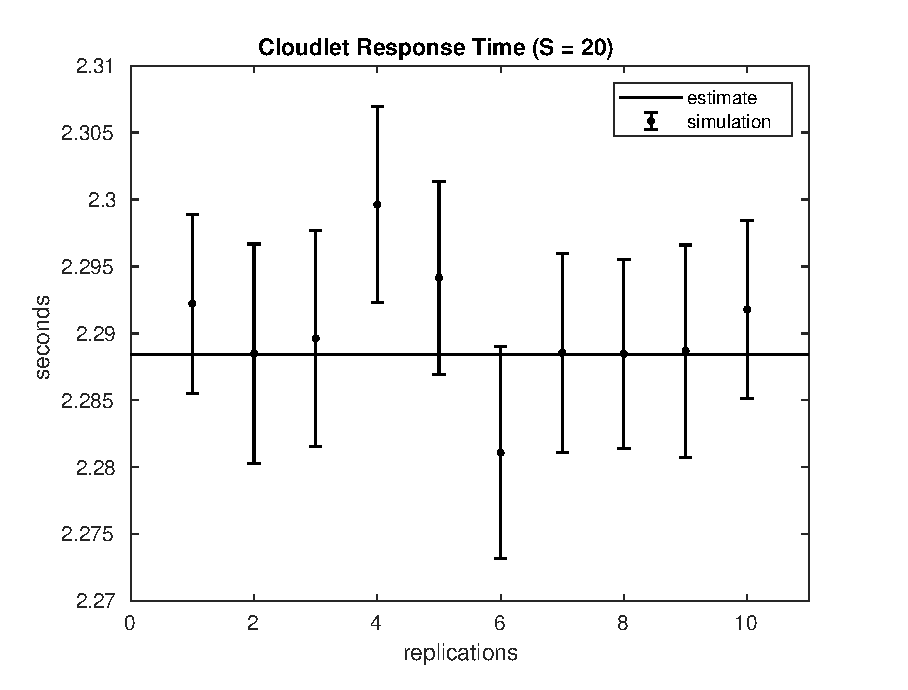
\includegraphics[width=\textwidth]{figures/simul/20_500K_sclet}
\caption{$S = 20$}
\label{20_sclet}
\end{subfigure}
%
\begin{subfigure}[t]{0.49\textwidth}
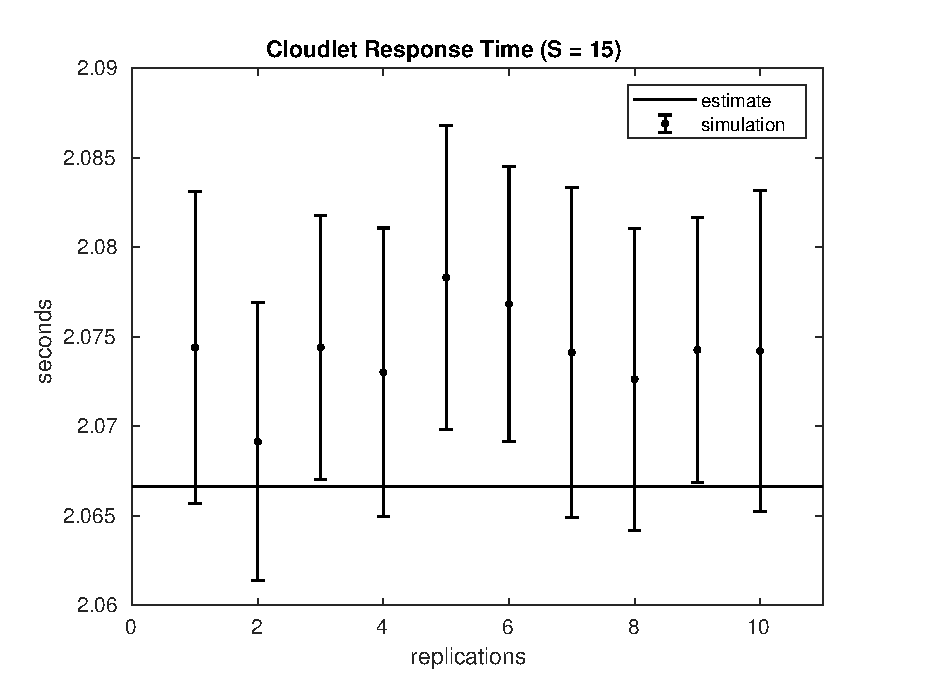
\includegraphics[width=\textwidth]{figures/simul/15_500K_sclet}
\caption{$S = 15$}
\label{15_sclet}
\end{subfigure}
%
\begin{subfigure}[t]{0.49\textwidth}
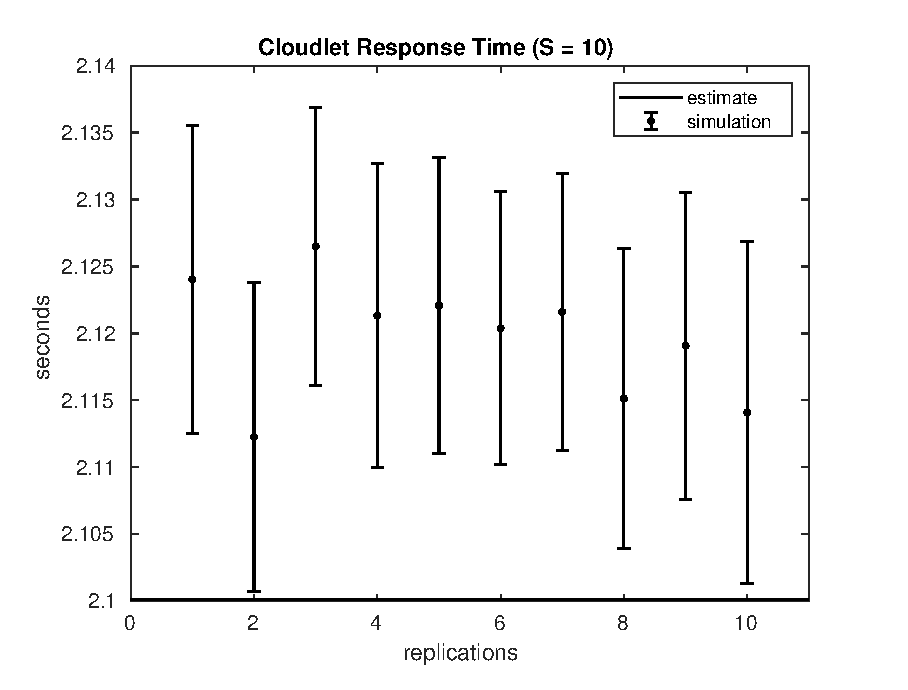
\includegraphics[width=\textwidth]{figures/simul/10_500K_sclet}
\caption{$S = 10$}
\label{10_sclet}
\end{subfigure}
%
\begin{subfigure}[t]{0.49\textwidth}
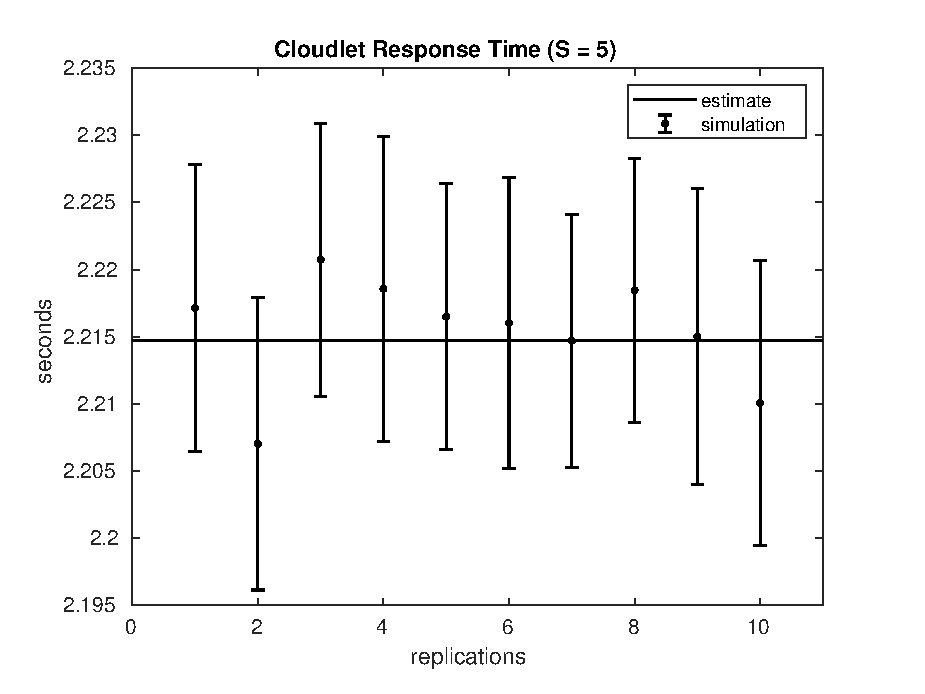
\includegraphics[width=\textwidth]{figures/simul/5_500K_sclet}
\caption{$S = 5$}
\label{5_sclet}
\end{subfigure}
%
\caption{tempo di risposta cloudlet}
\label{plot:sclet}
\end{figure}
%
%
\begin{table}[!h]
\begin{adjustbox}{width=\textwidth}
\begin{tabular}{c|r@{.}l|r@{.}l|r@{.}l|r@{.}l}
& \multicolumn{2}{|c|}{$S=20$}
& \multicolumn{2}{|c|}{$S=15$}
& \multicolumn{2}{|c|}{$S=10$}
& \multicolumn{2}{|c}{$S=5$}
\\          
\hline
R1      & $2$&$2922 \pm 0.0067$ & $2$&$0744 \pm 0.0087$ & $2$&$1240 \pm 0.0115$ & $2$&$2171 \pm 0.0107$ \\
R2      & $2$&$2885 \pm 0.0082$ & $2$&$0691 \pm 0.0078$ & $2$&$1123 \pm 0.0115$ & $2$&$2070 \pm 0.0109$ \\
R3      & $2$&$2896 \pm 0.0081$ & $2$&$0744 \pm 0.0074$ & $2$&$1265 \pm 0.0104$ & $2$&$2207 \pm 0.0102$ \\
R4      & $2$&$2996 \pm 0.0073$ & $2$&$0730 \pm 0.0081$ & $2$&$1213 \pm 0.0114$ & $2$&$2186 \pm 0.0113$ \\
R5      & $2$&$2942 \pm 0.0072$ & $2$&$0783 \pm 0.0085$ & $2$&$1221 \pm 0.0110$ & $2$&$2165 \pm 0.0099$ \\
R6      & $2$&$2811 \pm 0.0079$ & $2$&$0768 \pm 0.0077$ & $2$&$1204 \pm 0.0102$ & $2$&$2160 \pm 0.0108$ \\
R7      & $2$&$2885 \pm 0.0074$ & $2$&$0741 \pm 0.0092$ & $2$&$1216 \pm 0.0103$ & $2$&$2147 \pm 0.0094$ \\
R8      & $2$&$2885 \pm 0.0071$ & $2$&$0726 \pm 0.0084$ & $2$&$1151 \pm 0.0112$ & $2$&$2185 \pm 0.0098$ \\
R9      & $2$&$2887 \pm 0.0079$ & $2$&$0743 \pm 0.0074$ & $2$&$1191 \pm 0.0115$ & $2$&$2150 \pm 0.0110$ \\
R10     & $2$&$2918 \pm 0.0066$ & $2$&$0742 \pm 0.0090$ & $2$&$1141 \pm 0.0127$ & $2$&$2101 \pm 0.0106$ \\
EST     & $2$&$2884$            & $2$&$0666$            & $2$&$1002$            & $2$&$2147$            \\
\epsmx  & $0$&$0185 \ (0.8\%)$  & $0$&$0201 \ (1.0\%)$  & $0$&$0367 \ (1.7\%)$  & $0$&$0162 \ (0.7\%)$    
\end{tabular}
\end{adjustbox}
\caption{tempo di risposta cloudlet}
\label{tab:sclet}
\end{table}

%%%%%%%%%%%%%%%%%%%%%%%%%%%%%%%%%%%%%%%%%%%%%%%%%%%%%%%%%%%%%%%%%%%%%%%%%%%%%%%%
\subsection{Tempo di Risposta Cloud Classe 2}
Il tempo di risposta per un job di classe 2 che viene eseguito nel cloud è
indipendente dal parametro S ed i risultati presentati in
figura~\ref{plot:s2cloud} e nella tabella~\ref{tab:s2cloud} mostrano che tutti
gli intervalli di confidenza calcolati comprendono il valore stimato ed il
valore dell'errore massimo è sotto la soglia dell'$1\%$ in ogni caso.
\begin{figure}[!h]
\centering
%
\begin{subfigure}[t]{0.49\textwidth}
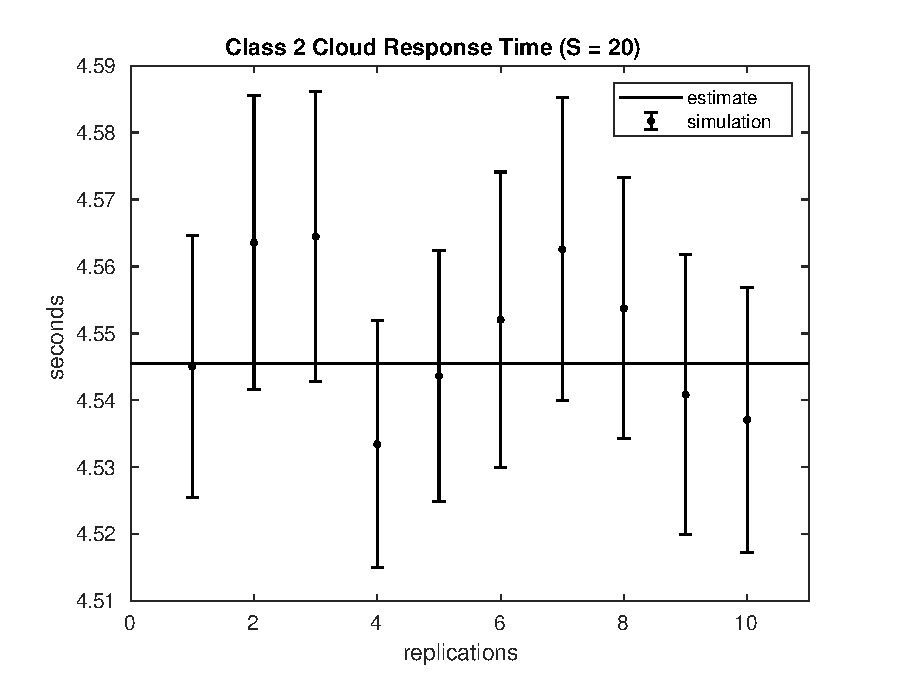
\includegraphics[width=\textwidth]{figures/simul/20_500K_s2cloud}
\caption{$S = 20$}
\label{20_s2cloud}
\end{subfigure}
%
\begin{subfigure}[t]{0.49\textwidth}
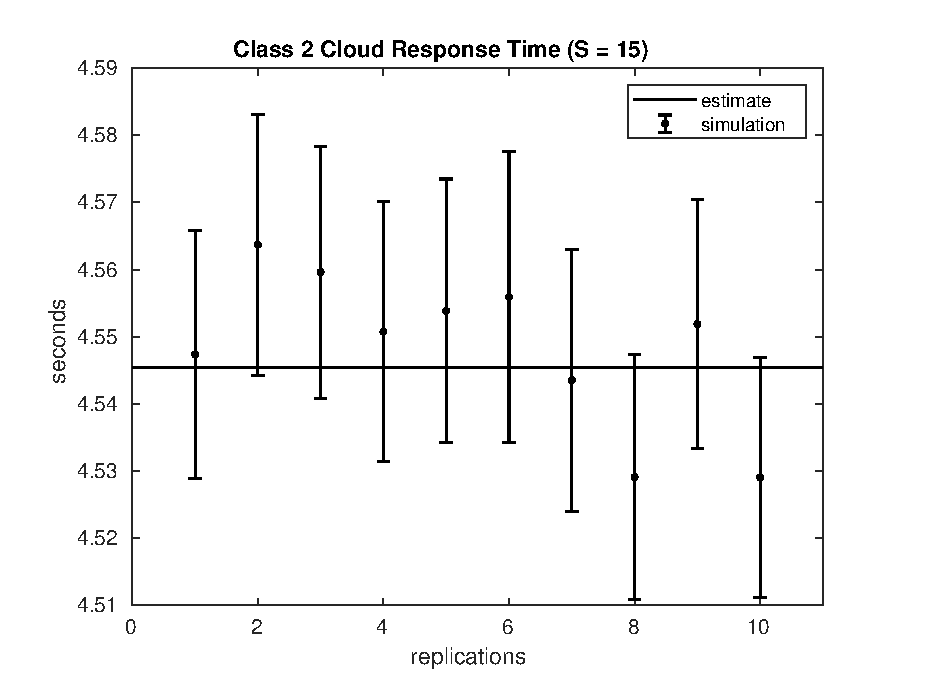
\includegraphics[width=\textwidth]{figures/simul/15_500K_s2cloud}
\caption{$S = 15$}
\label{15_s2cloud}
\end{subfigure}
%
\begin{subfigure}[t]{0.49\textwidth}
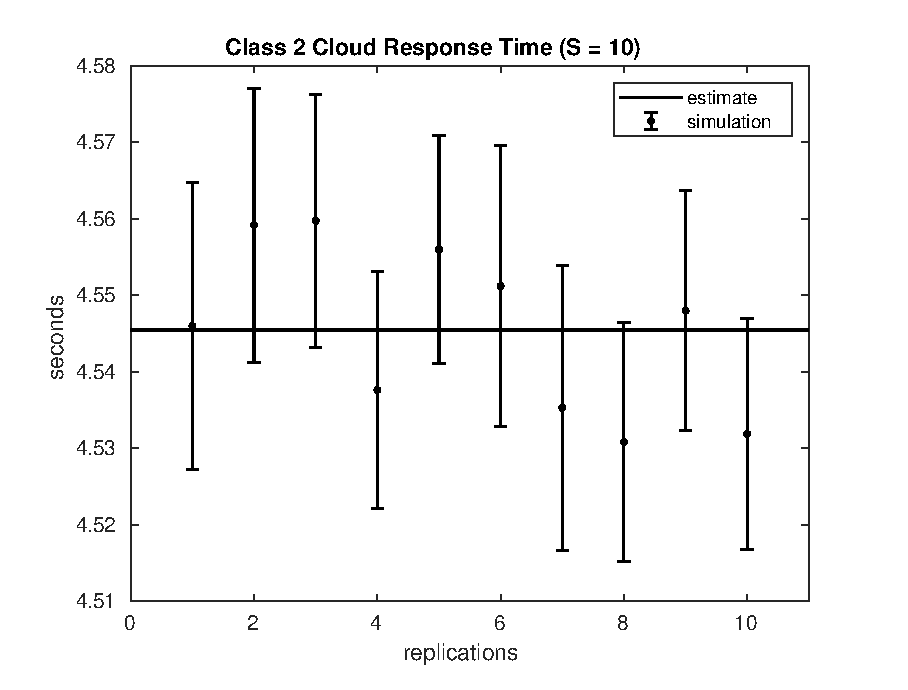
\includegraphics[width=\textwidth]{figures/simul/10_500K_s2cloud}
\caption{$S = 10$}
\label{10_s2cloud}
\end{subfigure}
%
\begin{subfigure}[t]{0.49\textwidth}
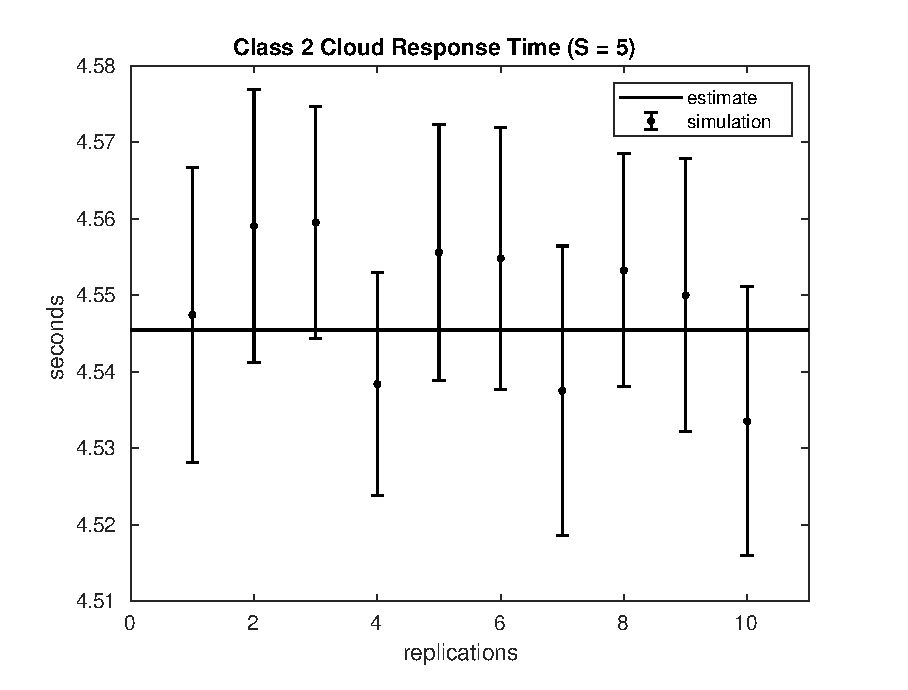
\includegraphics[width=\textwidth]{figures/simul/5_500K_s2cloud}
\caption{$S = 5$}
\label{5_s2cloud}
\end{subfigure}
%
\caption{tempo di risposta cloud classe 2}
\label{plot:s2cloud}
\end{figure}
%
%
\begin{table}[!h]
\begin{adjustbox}{width=\textwidth}
\begin{tabular}{c|r@{.}l|r@{.}l|r@{.}l|r@{.}l}
& \multicolumn{2}{|c|}{$S=20$}
& \multicolumn{2}{|c|}{$S=15$} 
& \multicolumn{2}{|c|}{$S=10$} 
& \multicolumn{2}{|c}{$S=5$} 
\\          
\hline
R1      & $4$&$5450 \pm 0.0196$  & $4$&$5474 \pm 0.0184$ & $4$&$5460 \pm 0.0188$ & $4$&$5474 \pm 0.0192$ \\
R2      & $4$&$5636 \pm 0.0219$  & $4$&$5637 \pm 0.0194$ & $4$&$5591 \pm 0.0179$ & $4$&$5590 \pm 0.0179$ \\
R3      & $4$&$5644 \pm 0.0216$  & $4$&$5596 \pm 0.0188$ & $4$&$5597 \pm 0.0165$ & $4$&$5595 \pm 0.0152$ \\
R4      & $4$&$5335 \pm 0.0185$  & $4$&$5507 \pm 0.0193$ & $4$&$5376 \pm 0.0154$ & $4$&$5384 \pm 0.0146$ \\
R5      & $4$&$5436 \pm 0.0187$  & $4$&$5538 \pm 0.0196$ & $4$&$5560 \pm 0.0148$ & $4$&$5556 \pm 0.0168$ \\
R6      & $4$&$5520 \pm 0.0221$  & $4$&$5559 \pm 0.0216$ & $4$&$5512 \pm 0.0183$ & $4$&$5548 \pm 0.0171$ \\
R7      & $4$&$5626 \pm 0.0226$  & $4$&$5435 \pm 0.0195$ & $4$&$5353 \pm 0.0186$ & $4$&$5375 \pm 0.0189$ \\
R8      & $4$&$5537 \pm 0.0195$  & $4$&$5291 \pm 0.0182$ & $4$&$5308 \pm 0.0156$ & $4$&$5533 \pm 0.0152$ \\
R9      & $4$&$5409 \pm 0.0209$  & $4$&$5519 \pm 0.0185$ & $4$&$5480 \pm 0.0157$ & $4$&$5500 \pm 0.0178$ \\
R10     & $4$&$5371 \pm 0.0197$  & $4$&$5291 \pm 0.0179$ & $4$&$5319 \pm 0.0151$ & $4$&$5335 \pm 0.0176$ \\
EST     & $4$&$5455$             & $4$&$5455$            & $4$&$5455$            & $4$&$5455$            \\
\epsmx  & $0$&$0406 \ (0.9\%)$   & $0$&$0376 \ (0.8\%)$  & $0$&$0316 \ (0.7\%)$  & $0$&$0314 \ (0.7\%)$    
\end{tabular}
\end{adjustbox}
\caption{tempo di risposta cloud classe 2}
\label{tab:s2cloud}
\end{table}

%%%%%%%%%%%%%%%%%%%%%%%%%%%%%%%%%%%%%%%%%%%%%%%%%%%%%%%%%%%%%%%%%%%%%%%%%%%%%%%%%
\subsection{Tempo di Risposta Cloud}
Il tempo di risposta del cloud è completamente dominato dai job di classe 2,
infatti, come mostrano la figura~\ref{plot:scloud} e la
tabella~\ref{tab:scloud}, i risultati sono pressoché identici alla precedente
metrica.
\begin{figure}[!h]
\centering
%
\begin{subfigure}[t]{0.49\textwidth}
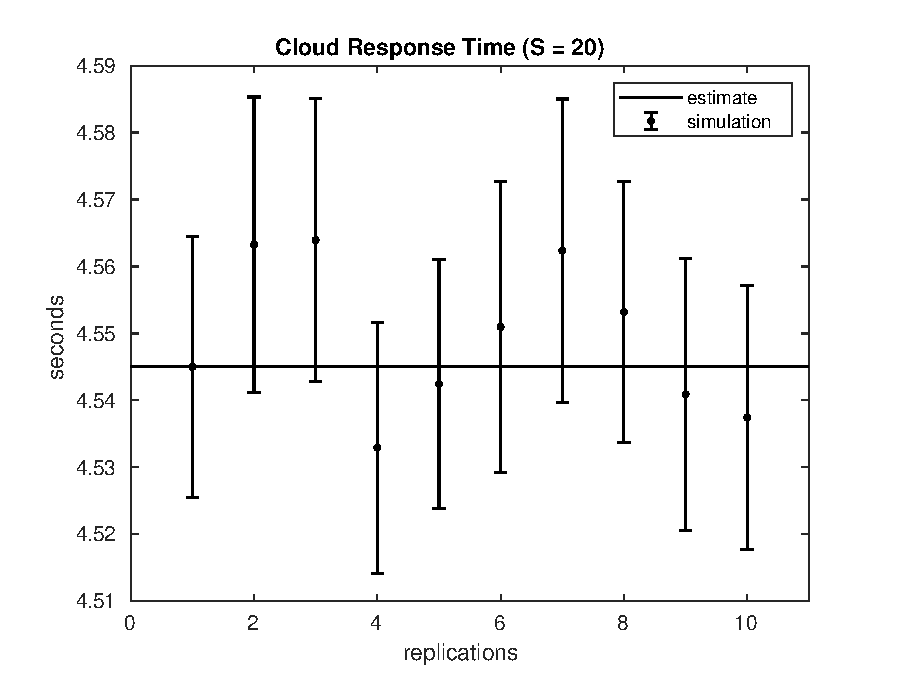
\includegraphics[width=\textwidth]{figures/simul/20_500K_scloud}
\caption{$S = 20$}
\label{20_scloud}
\end{subfigure}
%
\begin{subfigure}[t]{0.49\textwidth}
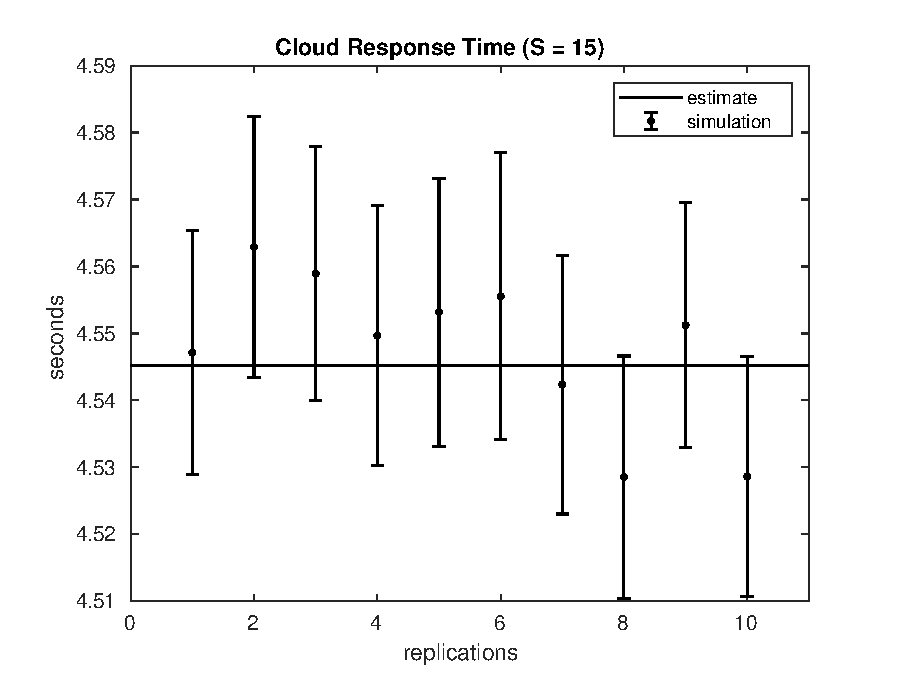
\includegraphics[width=\textwidth]{figures/simul/15_500K_scloud}
\caption{$S = 15$}
\label{15_scloud}
\end{subfigure}
%
\begin{subfigure}[t]{0.49\textwidth}
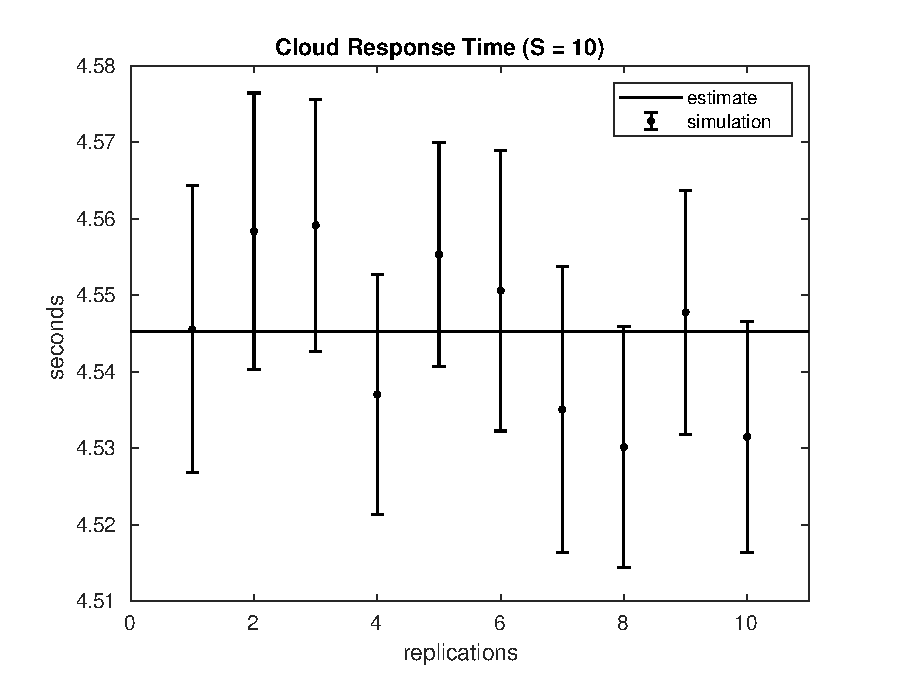
\includegraphics[width=\textwidth]{figures/simul/10_500K_scloud}
\caption{$S = 10$}
\label{10_scloud}
\end{subfigure}
%
\begin{subfigure}[t]{0.49\textwidth}
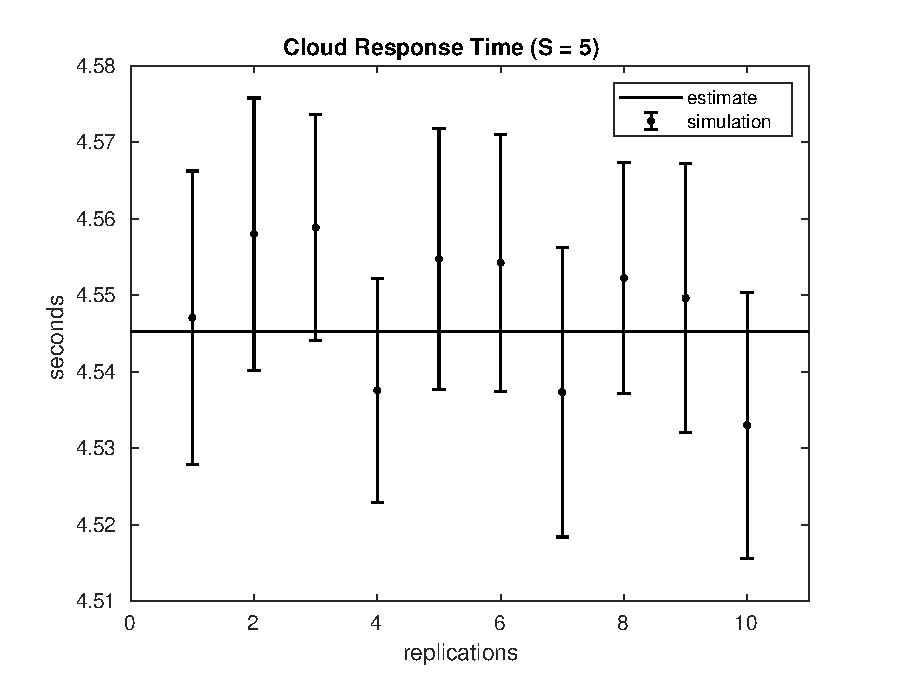
\includegraphics[width=\textwidth]{figures/simul/5_500K_scloud}
\caption{$S = 5$}
\label{5_scloud}
\end{subfigure}
%
\caption{tempo di risposta cloud}
\label{plot:scloud}
\end{figure}
%
%
\begin{table}[!h]
\begin{adjustbox}{width=\textwidth}
\begin{tabular}{c|r@{.}l|r@{.}l|r@{.}l|r@{.}l}
& \multicolumn{2}{|c|}{$S=20$}
& \multicolumn{2}{|c|}{$S=15$} 
& \multicolumn{2}{|c|}{$S=10$} 
& \multicolumn{2}{|c}{$S=5$} 
\\          
\hline
R1      & $4$&$5450 \pm 0.0195$ & $4$&$5471 \pm 0.0182$ & $4$&$5455 \pm 0.0187$ & $4$&$5471 \pm 0.0192$ \\
R2      & $4$&$5633 \pm 0.0220$ & $4$&$5629 \pm 0.0195$ & $4$&$5583 \pm 0.0181$ & $4$&$5580 \pm 0.0178$ \\
R3      & $4$&$5639 \pm 0.0211$ & $4$&$5589 \pm 0.0189$ & $4$&$5591 \pm 0.0164$ & $4$&$5588 \pm 0.0147$ \\
R4      & $4$&$5329 \pm 0.0188$ & $4$&$5497 \pm 0.0194$ & $4$&$5370 \pm 0.0157$ & $4$&$5376 \pm 0.0146$ \\
R5      & $4$&$5424 \pm 0.0185$ & $4$&$5532 \pm 0.0200$ & $4$&$5553 \pm 0.0146$ & $4$&$5548 \pm 0.0170$ \\
R6      & $4$&$5510 \pm 0.0217$ & $4$&$5555 \pm 0.0214$ & $4$&$5506 \pm 0.0183$ & $4$&$5542 \pm 0.0168$ \\
R7      & $4$&$5624 \pm 0.0226$ & $4$&$5424 \pm 0.0193$ & $4$&$5351 \pm 0.0186$ & $4$&$5373 \pm 0.0189$ \\
R8      & $4$&$5532 \pm 0.0195$ & $4$&$5286 \pm 0.0181$ & $4$&$5301 \pm 0.0158$ & $4$&$5523 \pm 0.0151$ \\
R9      & $4$&$5409 \pm 0.0204$ & $4$&$5512 \pm 0.0183$ & $4$&$5478 \pm 0.0159$ & $4$&$5496 \pm 0.0175$ \\
R10     & $4$&$5374 \pm 0.0197$ & $4$&$5287 \pm 0.0179$ & $4$&$5315 \pm 0.0151$ & $4$&$5330 \pm 0.0174$ \\
EST     & $4$&$5451$            & $4$&$5452$            & $4$&$5453$            & $4$&$5453$            \\
\epsmx  & $0$&$0402 \ (0.9\%)$  & $0$&$0372 \ (0.8\%)$  & $0$&$0312 \ (0.7\%)$  & $0$&$0305 \ (0.7\%)$    
\end{tabular}
\end{adjustbox}
\caption{tempo di risposta cloud}
\label{tab:scloud}
\end{table}

%%%%%%%%%%%%%%%%%%%%%%%%%%%%%%%%%%%%%%%%%%%%%%%%%%%%%%%%%%%%%%%%%%%%%%%%%%%%%%%%
\subsection{Tempo di Risposta Job Interrotti}
La figura~\ref{plot:sintr} e la tabella~\ref{tab:sintr}, confermano che il tempo
di risposta dei job interrotti ha un andamento analogo al tempo di risposta
medio dei job di classe 2 processati con successo nel cloudlet, infatti si nota
che tale tempo è direttamente proporzionale al parametro di soglia, quindi
inversamente proporzionale alla probabilità di interruzione.

Effettuando un confronto con i tempi di risposta del cloudlet, ci si rende conto
di quanto costi l'interruzione di un job ed è quindi lecito aspettarsi che
queste interruzioni incidano in maniera significativa sul tempo di risposta dei
job di classe 2 del sistema.

Anche l'errore massimo che si è commesso con la stima della statistiche, sembra
crescere con $S$, infatti per $S=5$ si ha un errore massimo dell'$1.1\%$ che
cresce fino ad arrivare al $2.5\%$ nel caso in cui $S=20$. 
\begin{figure}[!h]
\centering
%
\begin{subfigure}[t]{0.49\textwidth}
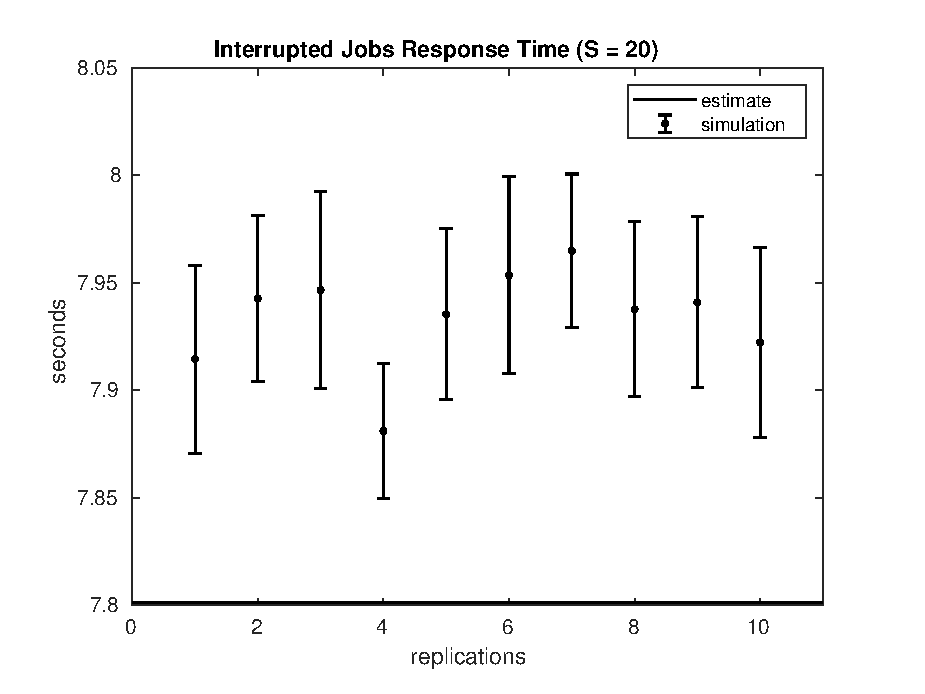
\includegraphics[width=\textwidth]{figures/simul/20_500K_sintr}
\caption{$S = 20$}
\label{20_sintr}
\end{subfigure}
%
\begin{subfigure}[t]{0.49\textwidth}
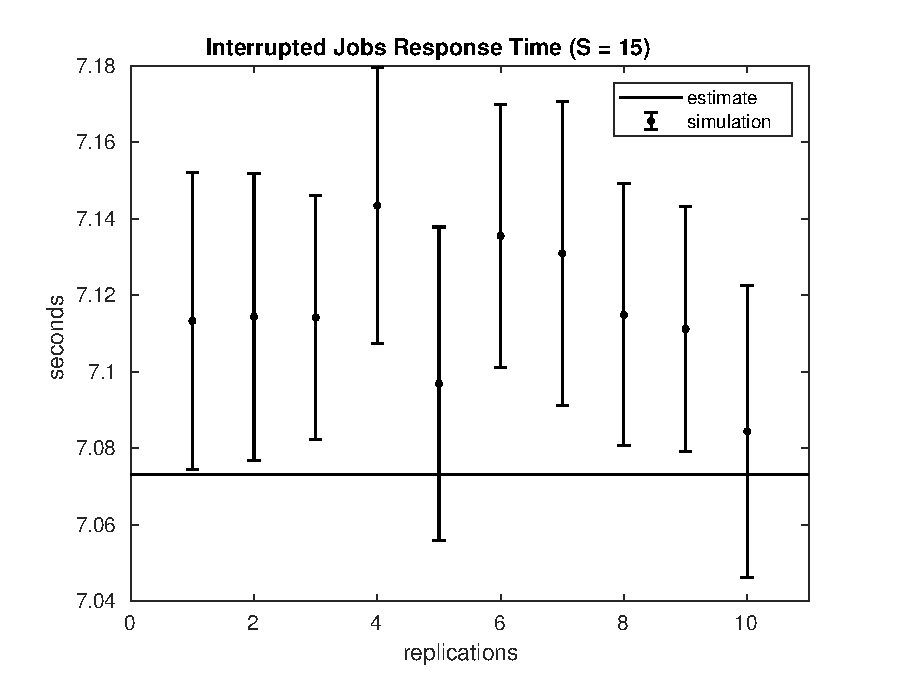
\includegraphics[width=\textwidth]{figures/simul/15_500K_sintr}
\caption{$S = 15$}
\label{15_sintr}
\end{subfigure}
%
\begin{subfigure}[t]{0.49\textwidth}
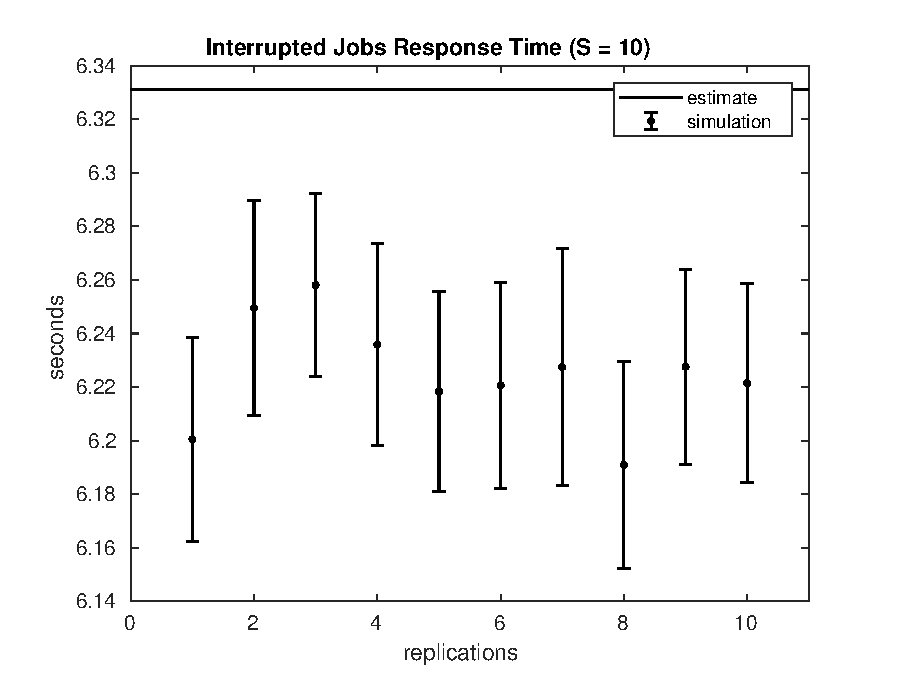
\includegraphics[width=\textwidth]{figures/simul/10_500K_sintr}
\caption{$S = 10$}
\label{10_sintr}
\end{subfigure}
%
\begin{subfigure}[t]{0.49\textwidth}
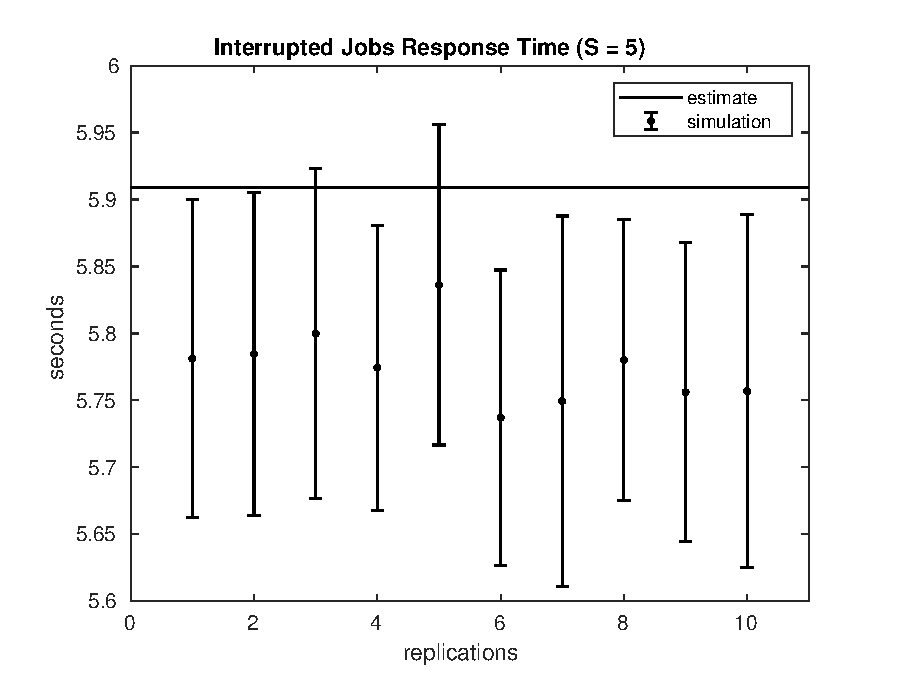
\includegraphics[width=\textwidth]{figures/simul/5_500K_sintr}
\caption{$S = 5$}
\label{5_sintr}
\end{subfigure}
%
\caption{tempo di risposta job interrotti}
\label{plot:sintr}
\end{figure}
%
%
\begin{table}[!h]
\begin{adjustbox}{width=\textwidth}
\begin{tabular}{c|r@{.}l|r@{.}l|r@{.}l|r@{.}l}
& \multicolumn{2}{|c|}{$S=20$}
& \multicolumn{2}{|c|}{$S=15$} 
& \multicolumn{2}{|c|}{$S=10$} 
& \multicolumn{2}{|c}{$S=5$} 
\\          
\hline
R1      & $7$&$9146 \pm 0.0437$  & $7$&$1133 \pm 0.0388$ & $6$&$2006 \pm 0.0381$ & $5$&$7813 \pm 0.1190$ \\
R2      & $7$&$9427 \pm 0.0387$  & $7$&$1144 \pm 0.0374$ & $6$&$2496 \pm 0.0401$ & $5$&$7846 \pm 0.1207$ \\
R3      & $7$&$9467 \pm 0.0458$  & $7$&$1142 \pm 0.0319$ & $6$&$2580 \pm 0.0342$ & $5$&$7998 \pm 0.1230$ \\
R4      & $7$&$8812 \pm 0.0312$  & $7$&$1434 \pm 0.0361$ & $6$&$2358 \pm 0.0377$ & $5$&$7744 \pm 0.1065$ \\
R5      & $7$&$9354 \pm 0.0398$  & $7$&$0969 \pm 0.0409$ & $6$&$2184 \pm 0.0373$ & $5$&$8362 \pm 0.1194$ \\
R6      & $7$&$9536 \pm 0.0457$  & $7$&$1355 \pm 0.0343$ & $6$&$2206 \pm 0.0383$ & $5$&$7372 \pm 0.1102$ \\
R7      & $7$&$9649 \pm 0.0358$  & $7$&$1309 \pm 0.0398$ & $6$&$2275 \pm 0.0441$ & $5$&$7496 \pm 0.1381$ \\
R8      & $7$&$9377 \pm 0.0407$  & $7$&$1149 \pm 0.0343$ & $6$&$1910 \pm 0.0386$ & $5$&$7802 \pm 0.1045$ \\
R9      & $7$&$9410 \pm 0.0397$  & $7$&$1112 \pm 0.0319$ & $6$&$2276 \pm 0.0365$ & $5$&$7562 \pm 0.1116$ \\
R10     & $7$&$9223 \pm 0.0443$  & $7$&$0844 \pm 0.0381$ & $6$&$2215 \pm 0.0372$ & $5$&$7570 \pm 0.1319$ \\
EST     & $7$&$8016$             & $7$&$0733$            & $6$&$3310$            & $5$&$9087$            \\
\epsmx  & $0$&$1991 \ (2.5\%)$   & $0$&$1062 \ (1.5\%)$  & $0$&$1015 \ (1.6\%)$  & $0$&$0614 \ (1.1\%)$    
\end{tabular}
\end{adjustbox}
\caption{tempo di risposta job interrotti}
\label{tab:sintr}
\end{table}

%%%%%%%%%%%%%%%%%%%%%%%%%%%%%%%%%%%%%%%%%%%%%%%%%%%%%%%%%%%%%%%%%%%%%%%%%%%%%%%%
\subsection{Tempo di Risposta Sistema Classe 1}
Il tempo di risposta globale dei job di classe 1 è completamente dominato dal
tempo di risposta dei job processati nel cloudlet, essendo molto minore il
numero di quelli eseguiti nel cloud. Infatti la figura~\ref{plot:s1} e la
tabella~\ref{tab:s1} mostrano delle statistiche pressoché identiche a quelle
relative al tempo di risposta dei job di classe 1 eseguiti nel coudlet, con un
errore massimo inferiore all'$1\%$.
\begin{figure}[!h]
\centering
%
\begin{subfigure}[t]{0.49\textwidth}
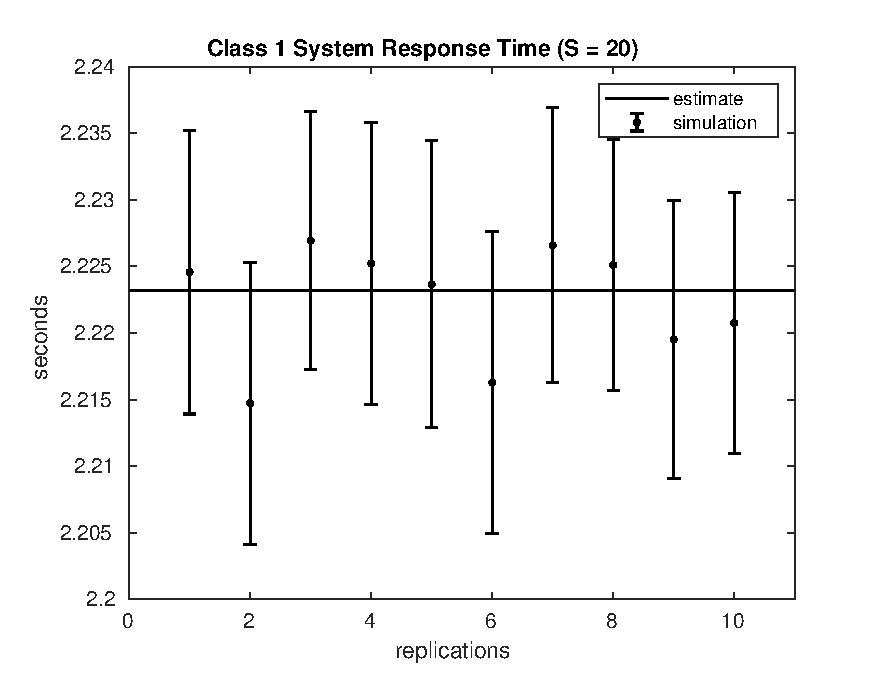
\includegraphics[width=\textwidth]{figures/simul/20_500K_s1}
\caption{$S = 20$}
\label{20_s1}
\end{subfigure}
%
\begin{subfigure}[t]{0.49\textwidth}
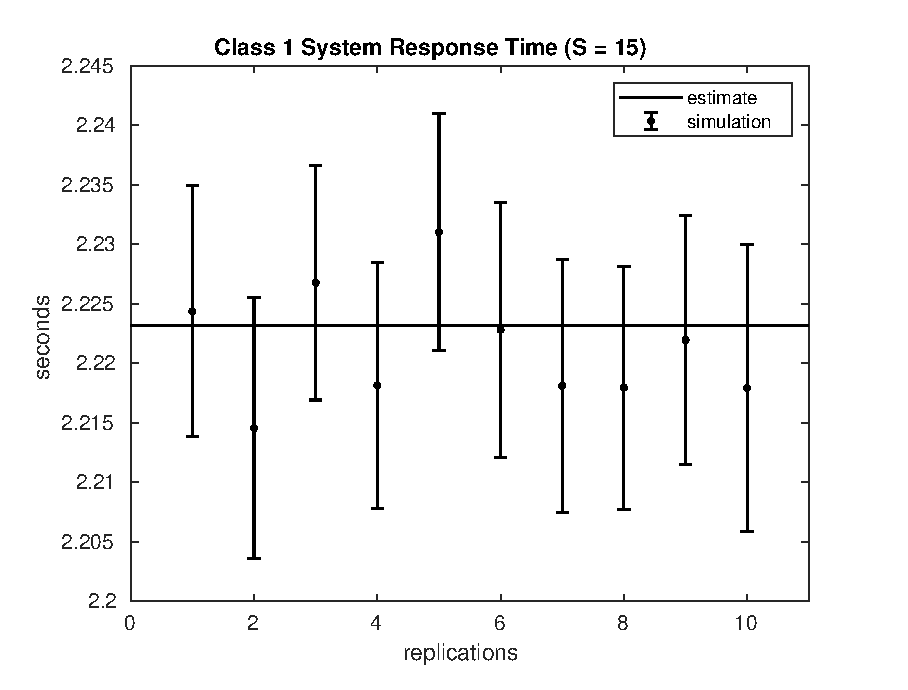
\includegraphics[width=\textwidth]{figures/simul/15_500K_s1}
\caption{$S = 15$}
\label{15_s1}
\end{subfigure}
%
\begin{subfigure}[t]{0.49\textwidth}
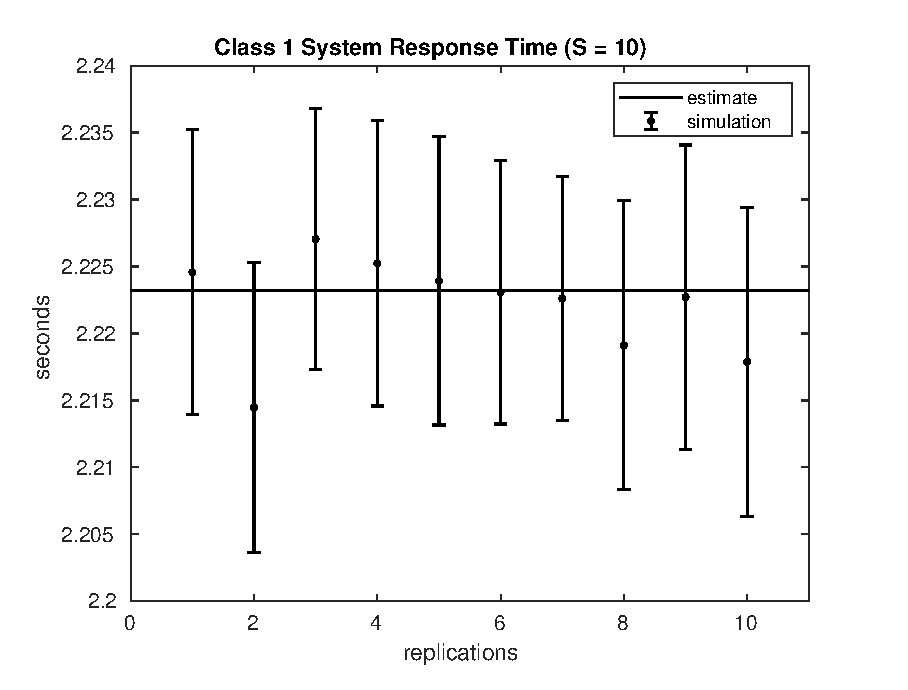
\includegraphics[width=\textwidth]{figures/simul/10_500K_s1}
\caption{$S = 10$}
\label{10_s1}
\end{subfigure}
%
\begin{subfigure}[t]{0.49\textwidth}
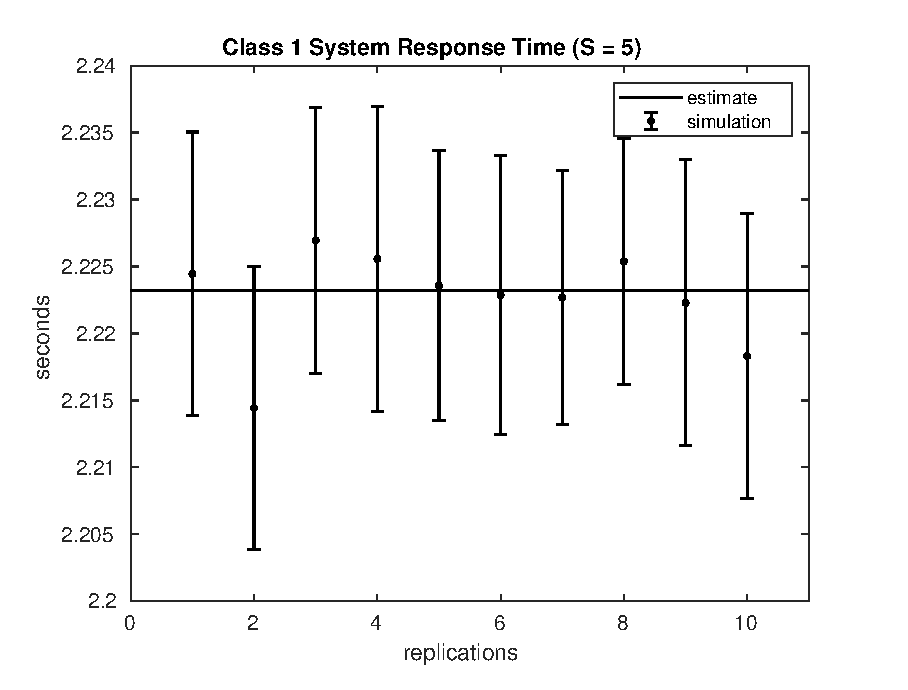
\includegraphics[width=\textwidth]{figures/simul/5_500K_s1}
\caption{$S = 5$}
\label{5_s1}
\end{subfigure}
%
\caption{tempo di risposta sistema classe 1}
\label{plot:s1}
\end{figure}
%
%
\begin{table}[!h]
\begin{adjustbox}{width=\textwidth}
\begin{tabular}{c|r@{.}l|r@{.}l|r@{.}l|r@{.}l}
& \multicolumn{2}{|c|}{$S=20$}
& \multicolumn{2}{|c|}{$S=15$} 
& \multicolumn{2}{|c|}{$S=10$} 
& \multicolumn{2}{|c}{$S=5$} 
\\          
\hline
R1      & $2$&$2246 \pm 0.0107$ & $2$&$2244 \pm 0.0105$ & $2$&$2246 \pm 0.0107$ & $2$&$2245 \pm 0.0106$ \\
R2      & $2$&$2147 \pm 0.0106$ & $2$&$2145 \pm 0.0110$ & $2$&$2145 \pm 0.0108$ & $2$&$2144 \pm 0.0106$ \\
R3      & $2$&$2269 \pm 0.0097$ & $2$&$2268 \pm 0.0098$ & $2$&$2270 \pm 0.0098$ & $2$&$2270 \pm 0.0099$ \\
R4      & $2$&$2252 \pm 0.0106$ & $2$&$2181 \pm 0.0103$ & $2$&$2252 \pm 0.0106$ & $2$&$2256 \pm 0.0114$ \\
R5      & $2$&$2237 \pm 0.0108$ & $2$&$2310 \pm 0.0100$ & $2$&$2239 \pm 0.0108$ & $2$&$2236 \pm 0.0101$ \\
R6      & $2$&$2163 \pm 0.0113$ & $2$&$2228 \pm 0.0107$ & $2$&$2231 \pm 0.0098$ & $2$&$2229 \pm 0.0104$ \\
R7      & $2$&$2266 \pm 0.0103$ & $2$&$2181 \pm 0.0106$ & $2$&$2226 \pm 0.0091$ & $2$&$2227 \pm 0.0095$ \\
R8      & $2$&$2251 \pm 0.0094$ & $2$&$2180 \pm 0.0102$ & $2$&$2191 \pm 0.0108$ & $2$&$2254 \pm 0.0092$ \\
R9      & $2$&$2195 \pm 0.0104$ & $2$&$2220 \pm 0.0104$ & $2$&$2227 \pm 0.0114$ & $2$&$2223 \pm 0.0107$ \\
R10     & $2$&$2208 \pm 0.0098$ & $2$&$2179 \pm 0.0120$ & $2$&$2179 \pm 0.0115$ & $2$&$2183 \pm 0.0107$ \\
EST     & $2$&$2232$            & $2$&$2232$            & $2$&$2232$            & $2$&$2232$            \\
\epsmx  & $0$&$0137 \ (0.6\%)$  & $0$&$0178 \ (0.8\%)$  & $0$&$0136 \ (0.6\%)$  & $0$&$0138 \ (0.6\%)$    
\end{tabular}
\end{adjustbox}
\caption{tempo di risposta sistema classe 1}
\label{tab:s1}
\end{table}

%%%%%%%%%%%%%%%%%%%%%%%%%%%%%%%%%%%%%%%%%%%%%%%%%%%%%%%%%%%%%%%%%%%%%%%%%%%%%%%%%
\subsection{Tempo di Risposta Sistema Classe 2}
La figura~\ref{plot:s2} e la tabella~\ref{tab:s2} mostrano che, nei casi in cui
$S=10,15,20$, i risultati delle simulazioni che risultano essere leggermente
superiori alle stime del modello analitico. Questo può essere dovuto
al peso che esercitano i job interrotti nel calcolo, infatti si ritrova la
stessa sottostima per quanto riguarda le percentuali di job interrotti
mostrate all'inizio, ma con un errore massimo minore (al più del $3.5\%$).
Inoltre nel caso in cui $S=5$, si ha una stima precisa con un errore massimo
dello $0.7\%$ perché vi sono un bassissimo numero di interruzioni.

Può essere interessante notare che si ottiene il minor tempo di risposta nello
scenario per cui $S=20$, nel quale si sperimenta il massimo tempo di risposta
dei job interrotti e una percentuale di interruzioni più alta del caso in cui si
sperimenta un tempo di risposta più basso per i job interrotti($S=10$). È
evidente quindi che acquista un peso significativo anche il tempo di esecuzione
nel cloud per quei job che ci finiscono direttamente, infatti nel caso in cui
$S=5$, nonostante soltanto circa il $2\%$ dei job viene interrotto, si registra
comunque un tempo paragonabile ai casi in cui ci sono maggiori interruzioni,
questo perché la maggior parte dei job di classe 2 viene direttamente inoltrata
al cloud.
\begin{figure}[!h]
\centering
%
\begin{subfigure}[t]{0.49\textwidth}
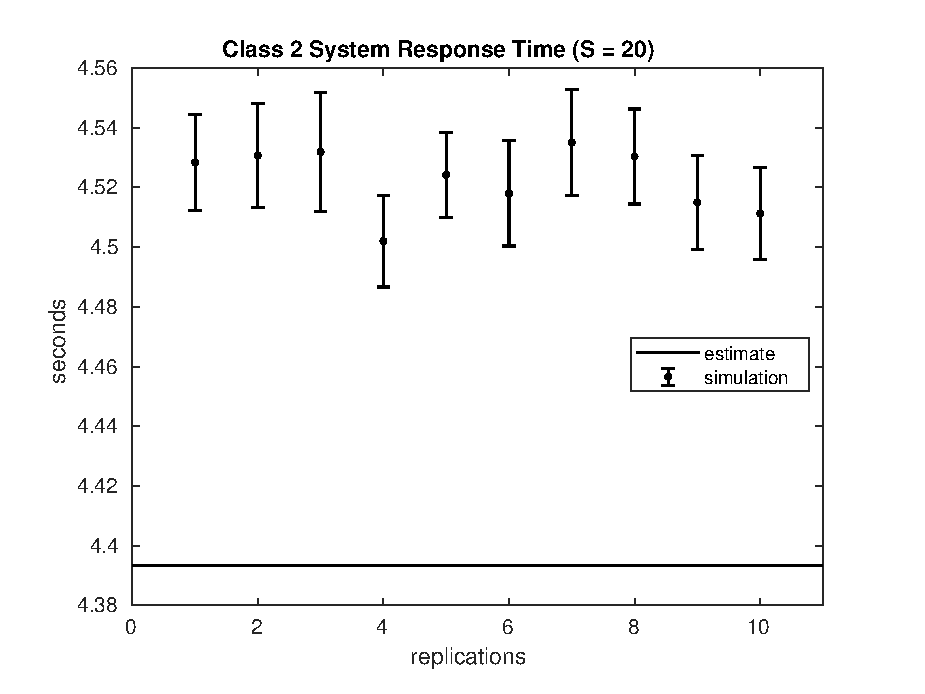
\includegraphics[width=\textwidth]{figures/simul/20_500K_s2}
\caption{$S = 20$}
\label{20_s2}
\end{subfigure}
%
\begin{subfigure}[t]{0.49\textwidth}
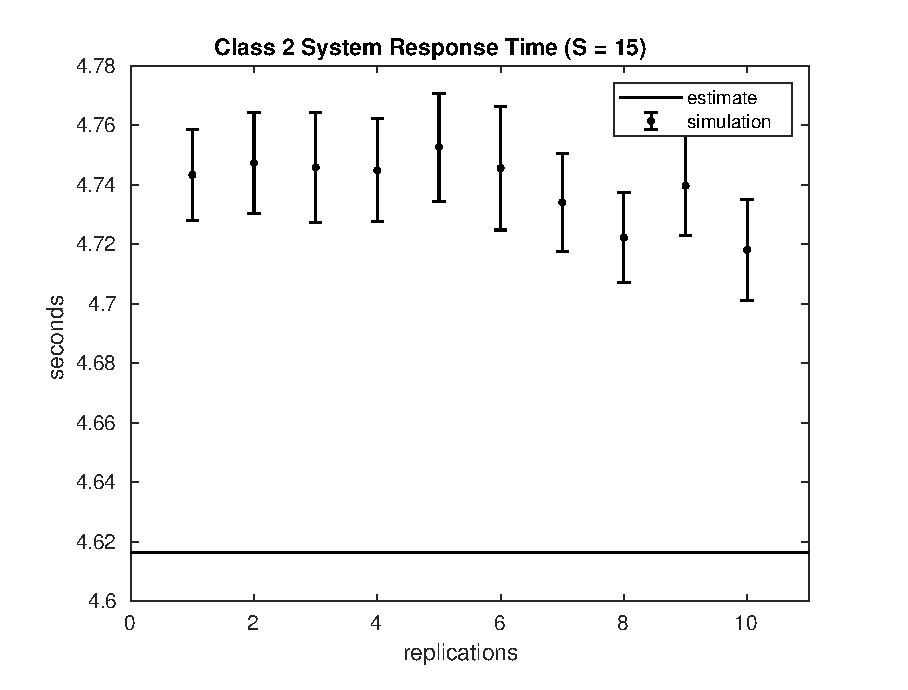
\includegraphics[width=\textwidth]{figures/simul/15_500K_s2}
\caption{$S = 15$}
\label{15_s2}
\end{subfigure}
%
\begin{subfigure}[t]{0.49\textwidth}
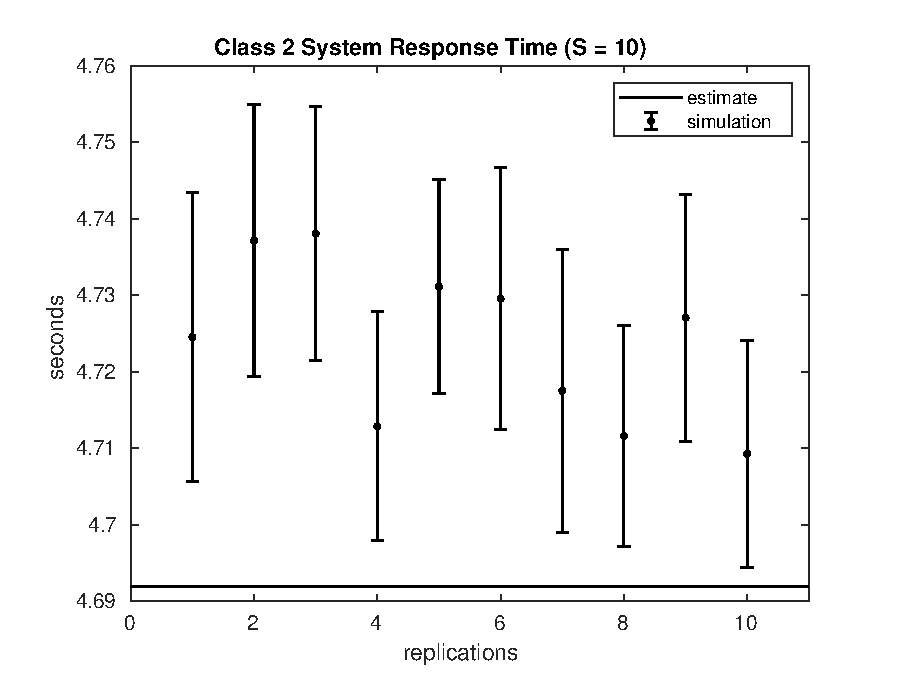
\includegraphics[width=\textwidth]{figures/simul/10_500K_s2}
\caption{$S = 10$}
\label{10_s2}
\end{subfigure}
%
\begin{subfigure}[t]{0.49\textwidth}
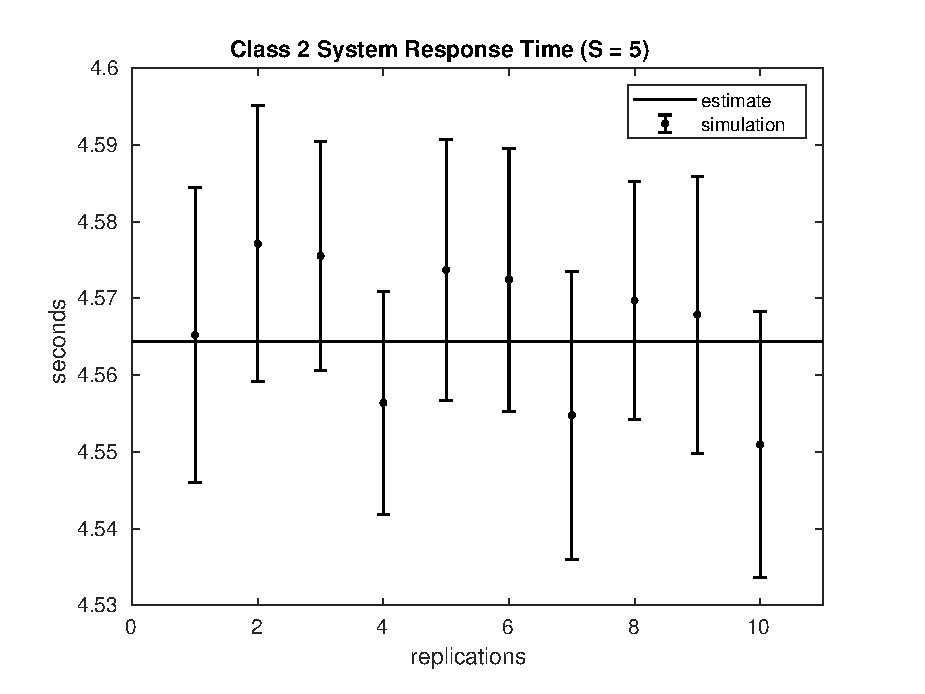
\includegraphics[width=\textwidth]{figures/simul/5_500K_s2}
\caption{$S = 5$}
\label{5_s2}
\end{subfigure}
%
\caption{tempo di risposta sistema classe 2}
\label{plot:s2}
\end{figure}
%
%
\begin{table}[!h]
\begin{adjustbox}{width=\textwidth}
\begin{tabular}{c|r@{.}l|r@{.}l|r@{.}l|r@{.}l}
& \multicolumn{2}{|c|}{$S=20$}
& \multicolumn{2}{|c|}{$S=15$} 
& \multicolumn{2}{|c|}{$S=10$} 
& \multicolumn{2}{|c}{$S=5$} 
\\          
\hline
R1      & $4$&$5284 \pm 0.0160$ & $4$&$7433 \pm 0.0154$ & $4$&$7245 \pm 0.0188$ & $4$&$5652 \pm 0.0192$ \\
R2      & $4$&$5307 \pm 0.0174$ & $4$&$7473 \pm 0.0170$ & $4$&$7371 \pm 0.0178$ & $4$&$5771 \pm 0.0180$ \\
R3      & $4$&$5319 \pm 0.0199$ & $4$&$7458 \pm 0.0185$ & $4$&$7381 \pm 0.0166$ & $4$&$5755 \pm 0.0149$ \\
R4      & $4$&$5020 \pm 0.0154$ & $4$&$7448 \pm 0.0173$ & $4$&$7129 \pm 0.0150$ & $4$&$5564 \pm 0.0145$ \\
R5      & $4$&$5242 \pm 0.0142$ & $4$&$7526 \pm 0.0181$ & $4$&$7311 \pm 0.0139$ & $4$&$5737 \pm 0.0170$ \\
R6      & $4$&$5180 \pm 0.0176$ & $4$&$7456 \pm 0.0208$ & $4$&$7295 \pm 0.0171$ & $4$&$5724 \pm 0.0171$ \\
R7      & $4$&$5351 \pm 0.0177$ & $4$&$7340 \pm 0.0164$ & $4$&$7175 \pm 0.0185$ & $4$&$5548 \pm 0.0187$ \\
R8      & $4$&$5303 \pm 0.0159$ & $4$&$7222 \pm 0.0151$ & $4$&$7116 \pm 0.0144$ & $4$&$5697 \pm 0.0155$ \\
R9      & $4$&$5150 \pm 0.0157$ & $4$&$7396 \pm 0.0168$ & $4$&$7271 \pm 0.0161$ & $4$&$5679 \pm 0.0180$ \\
R10     & $4$&$5113 \pm 0.0155$ & $4$&$7181 \pm 0.0170$ & $4$&$7093 \pm 0.0148$ & $4$&$5510 \pm 0.0173$ \\
EST     & $4$&$3935$            & $4$&$6165$            & $4$&$6920$            & $4$&$5644$            \\
\epsmx  & $0$&$1593 \ (3.5\%)$  & $0$&$1542 \ (3.2\%)$  & $0$&$0629 \ (1.3\%)$  & $0$&$0307 \ (0.7\%)$    
\end{tabular}
\end{adjustbox}
\caption{tempo di risposta sistema classe 2}
\label{tab:s2}
\end{table}

%%%%%%%%%%%%%%%%%%%%%%%%%%%%%%%%%%%%%%%%%%%%%%%%%%%%%%%%%%%%%%%%%%%%%%%%%%%%%%%%
\subsection{Tempo di Risposta Sistema}
Con l'aggiunta dei job di classe 1 nel calcolo del tempo di risposta globale del
sistema, la situazione non cambia, infatti, come mostrato in 
figura~\ref{plot:s} e tabella~\ref{tab:s}, si ottiene il minor tempo di risposta
nel caso in cui $S=20$, e anche in questo caso è evidente l'influenza della
percentuale di interruzione che induce alla sottostima, anche se con un errore
massimo più contenuto (al più del $2.7\%$), più precisa è invece la stima
del caso $S=5$ (\epsmx$=0.5\%$).

In conclusione si è ottenuto che per un valore di $S=20$ si ottiene il
tempo di risposta minimo pari a circa $3.61$ secondi, perché, con un alto
valore di soglia, si minimizzano gli inoltri diretti al cloud e si ha un numero
di interruzioni contenuto (non più del $24\%$ dei job di classe 2).

Nel caso in cui $S=15$ l'elevata percentuale di job interrotti ha influito
nell'ottenere un tempo di risposta maggiore rispetto agli altri casi, mentre per
un valore di soglia pari a $10$, nonostante il ridotto tempo di risposta dei job
interrotti e la bassa percentuale di interruzioni, si è ottenuto un tempo
maggiore dei casi $S=5,20$ per via dell'influenza dei job di classe 2 eseguiti
nel cloud

Per un valore di soglia $S=5$ si sperimenta un
elevato numero di inoltri diretti al server remoto ma al tempo stesso una
quantità minima di job interrotti, pertanto il tempo di risposta non è molto
lontano dal valore minimo che assume nel caso in cui $S=20$.

\begin{figure}[!h]
\centering
%
\begin{subfigure}[t]{0.49\textwidth}
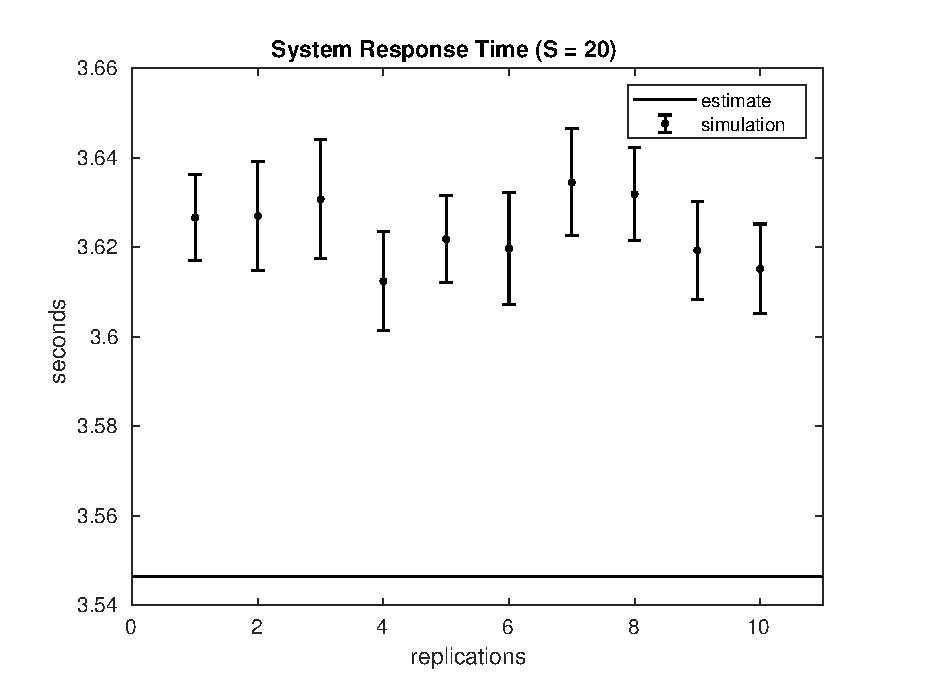
\includegraphics[width=\textwidth]{figures/simul/20_500K_s}
\caption{$S = 20$}
\label{20_s}
\end{subfigure}
%
\begin{subfigure}[t]{0.49\textwidth}
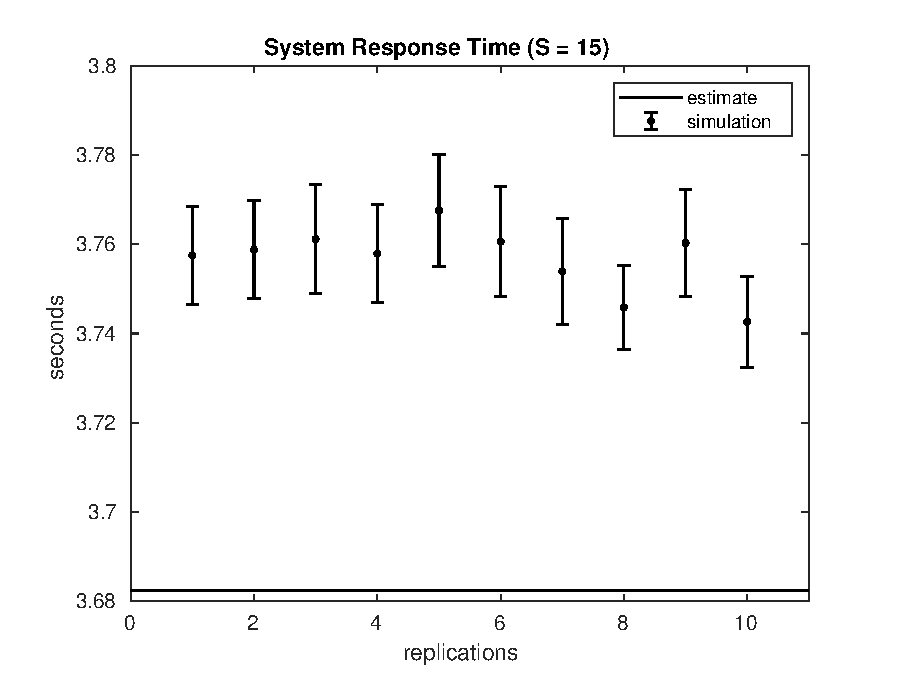
\includegraphics[width=\textwidth]{figures/simul/15_500K_s}
\caption{$S = 15$}
\label{15_s}
\end{subfigure}
%
\begin{subfigure}[t]{0.49\textwidth}
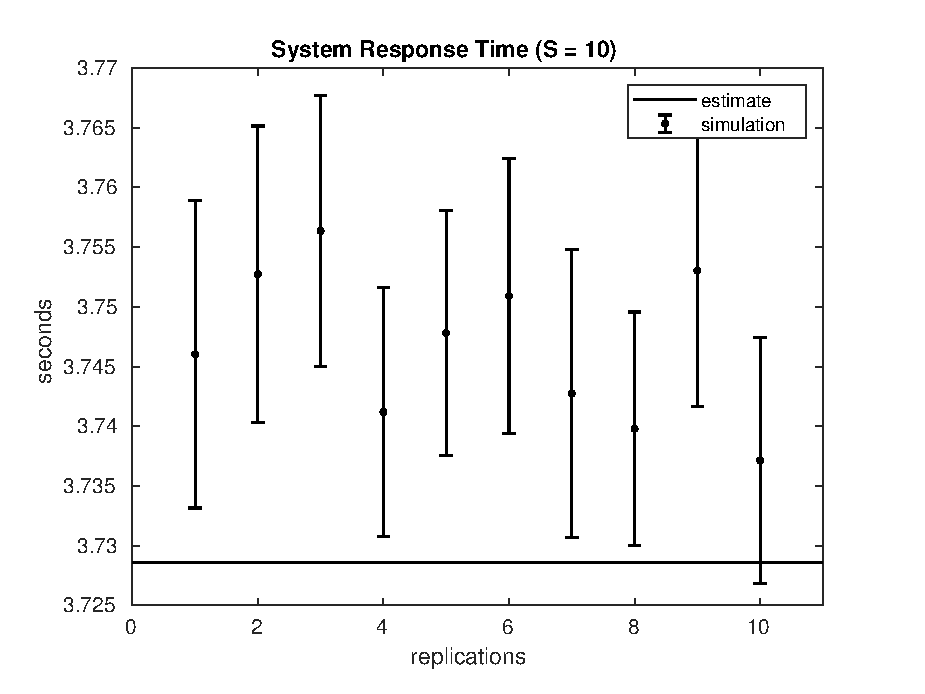
\includegraphics[width=\textwidth]{figures/simul/10_500K_s}
\caption{$S = 10$}
\label{10_s}
\end{subfigure}
%
\begin{subfigure}[t]{0.49\textwidth}
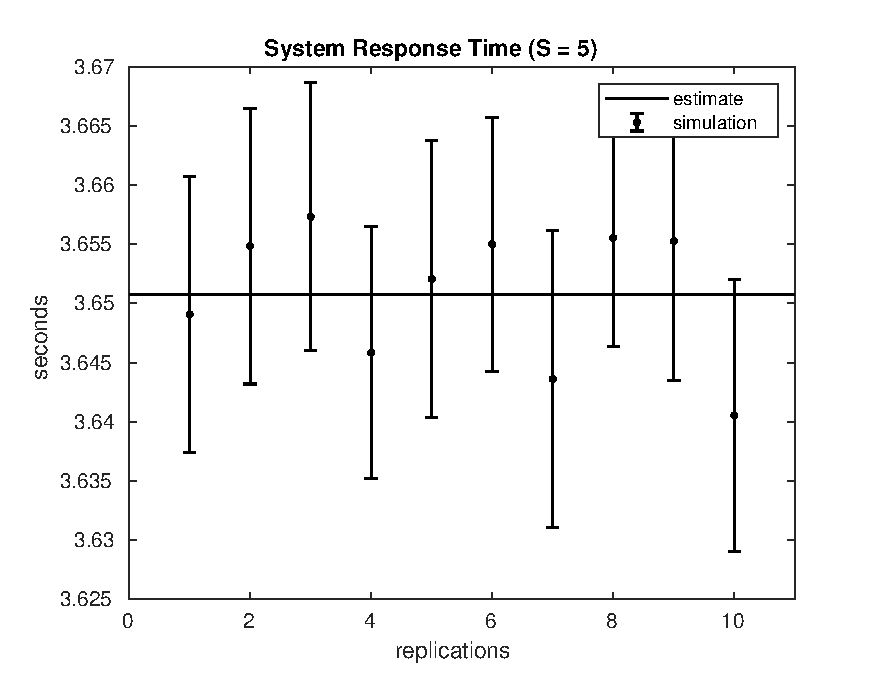
\includegraphics[width=\textwidth]{figures/simul/5_500K_s}
\caption{$S = 5$}
\label{5_s}
\end{subfigure}
%
\caption{tempo di risposta sistema}
\label{plot:s}
\end{figure}
%
%
\begin{table}[!h]
\begin{adjustbox}{width=\textwidth}
\begin{tabular}{c|r@{.}l|r@{.}l|r@{.}l|r@{.}l}
& \multicolumn{2}{|c|}{$S=20$}
& \multicolumn{2}{|c|}{$S=15$} 
& \multicolumn{2}{|c|}{$S=10$} 
& \multicolumn{2}{|c}{$S=5$} 
\\          
\hline
R1      & $3$&$6266 \pm 0.0096$ & $3$&$7575 \pm 0.0109$ & $3$&$7460 \pm 0.0129$ & $3$&$6491 \pm 0.0117$ \\
R2      & $3$&$6269 \pm 0.0121$ & $3$&$7588 \pm 0.0110$ & $3$&$7527 \pm 0.0124$ & $3$&$6548 \pm 0.0117$ \\
R3      & $3$&$6307 \pm 0.0133$ & $3$&$7611 \pm 0.0122$ & $3$&$7564 \pm 0.0114$ & $3$&$6573 \pm 0.0113$ \\
R4      & $3$&$6124 \pm 0.0110$ & $3$&$7579 \pm 0.0110$ & $3$&$7412 \pm 0.0105$ & $3$&$6458 \pm 0.0106$ \\
R5      & $3$&$6218 \pm 0.0097$ & $3$&$7675 \pm 0.0126$ & $3$&$7478 \pm 0.0103$ & $3$&$6521 \pm 0.0117$ \\
R6      & $3$&$6197 \pm 0.0125$ & $3$&$7606 \pm 0.0124$ & $3$&$7509 \pm 0.0115$ & $3$&$6550 \pm 0.0107$ \\
R7      & $3$&$6344 \pm 0.0119$ & $3$&$7539 \pm 0.0119$ & $3$&$7427 \pm 0.0120$ & $3$&$6436 \pm 0.0126$ \\
R8      & $3$&$6318 \pm 0.0103$ & $3$&$7459 \pm 0.0095$ & $3$&$7398 \pm 0.0098$ & $3$&$6555 \pm 0.0092$ \\
R9      & $3$&$6193 \pm 0.0109$ & $3$&$7603 \pm 0.0119$ & $3$&$7530 \pm 0.0114$ & $3$&$6553 \pm 0.0117$ \\
R10     & $3$&$6152 \pm 0.0100$ & $3$&$7426 \pm 0.0102$ & $3$&$7372 \pm 0.0103$ & $3$&$6406 \pm 0.0115$ \\
EST     & $3$&$5465$            & $3$&$6825$            & $3$&$7286$            & $3$&$6508$            \\
\epsmx  & $0$&$0999 \ (2.7\%)$  & $0$&$0976 \ (2.6\%)$  & $0$&$0392 \ (1.0\%)$  & $0$&$0179 \ (0.5\%)$    
\end{tabular}
\end{adjustbox}
\caption{tempo di risposta sistema}
\label{tab:s}
\end{table}

%%%%%%%%%%%%%%%%%%%%%%%%%%%%%%%%%%%%%%%%%%%%%%%%%%%%%%%%%%%%%%%%%%%%%%%%%%%%%%%%
%%%%%%%%%%%%%%%%%%%%%%%%%%%%%%%%%%%%%%%%%%%%%%%%%%%%%%%%%%%%%%%%%%%%%%%%%%%%%%%%
\subsection{Throughput Cloudlet Classe 1}
La figura~\ref{plot:x1clet} e la tabella~\ref{tab:x1clet} mostrano che il
throughput del cloudlet relativo ai job di classe 1 è pressoché costante al
variare del parametro $S$, ciò implica che l'evento in cui un job di classe 1
non viene accettato nel cloudlet avviente con probabilità remota in ogni caso.

La stima della statistica è affidabile con un errore massimo inferiore
all'$1\%$.  
\begin{figure}[!h]
\centering
%
\begin{subfigure}[t]{0.49\textwidth}
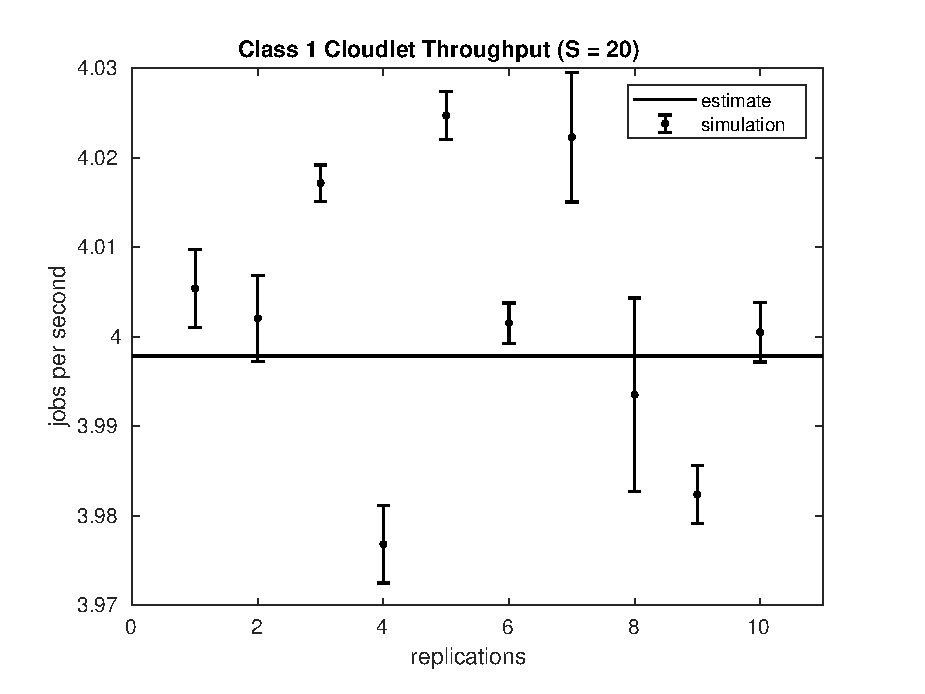
\includegraphics[width=\textwidth]{figures/simul/20_500K_x1clet}
\caption{$S = 20$}
\label{20_x1clet}
\end{subfigure}
%
\begin{subfigure}[t]{0.49\textwidth}
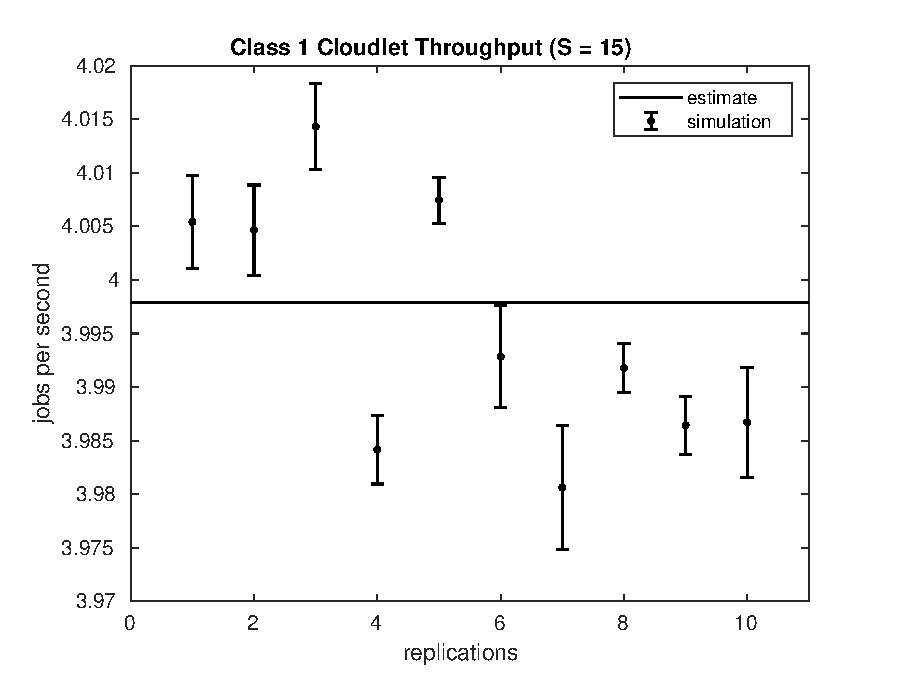
\includegraphics[width=\textwidth]{figures/simul/15_500K_x1clet}
\caption{$S = 15$}
\label{15_x1clet}
\end{subfigure}
%
\begin{subfigure}[t]{0.49\textwidth}
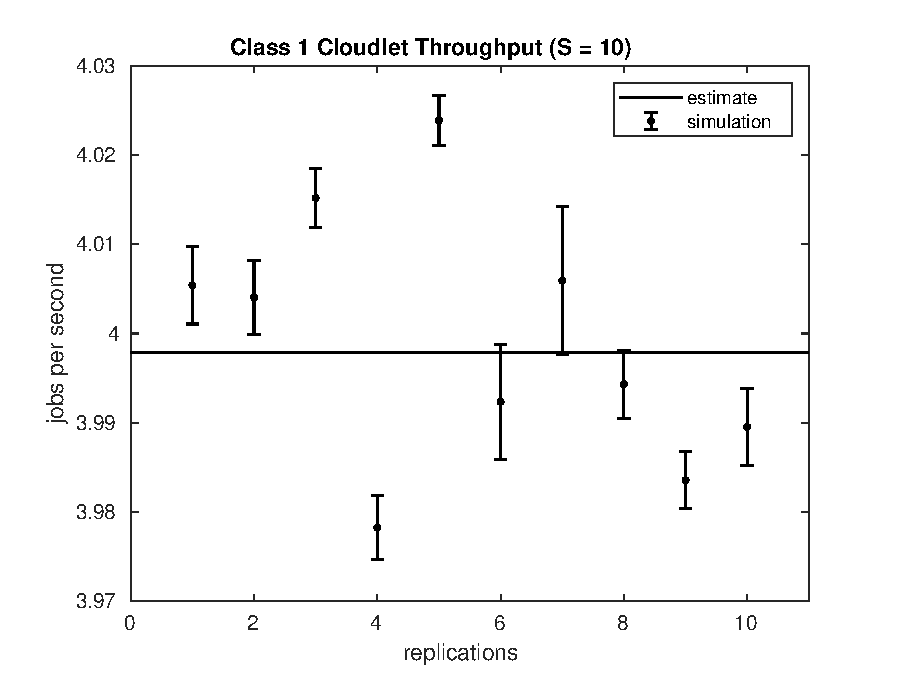
\includegraphics[width=\textwidth]{figures/simul/10_500K_x1clet}
\caption{$S = 10$}
\label{10_x1clet}
\end{subfigure}
%
\begin{subfigure}[t]{0.49\textwidth}
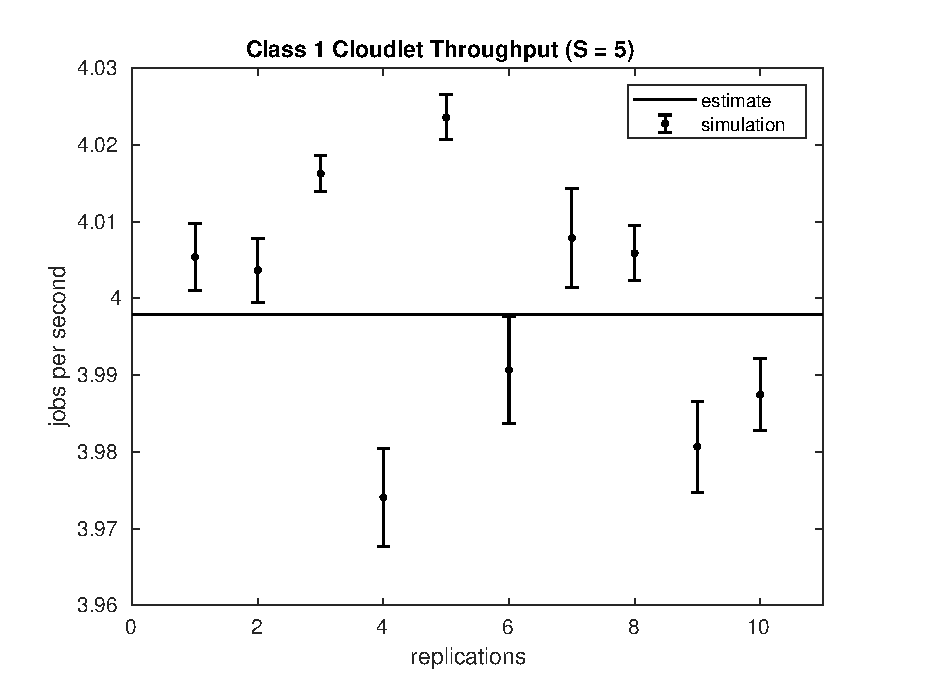
\includegraphics[width=\textwidth]{figures/simul/5_500K_x1clet}
\caption{$S = 5$}
\label{5_x1clet}
\end{subfigure}
%
\caption{throughput cloudlet classe 1}
\label{plot:x1clet}
\end{figure}
%
%
\begin{table}[!h]
\begin{adjustbox}{width=\textwidth}
\begin{tabular}{c|r@{.}l|r@{.}l|r@{.}l|r@{.}l}
& \multicolumn{2}{|c|}{$S=20$}
& \multicolumn{2}{|c|}{$S=15$}
& \multicolumn{2}{|c|}{$S=10$}
& \multicolumn{2}{|c}{$S=5$}
\\          
\hline
R1      & $4$&$0054 \pm 0.0043$ & $4$&$0054 \pm 0.0043$ & $4$&$0054 \pm 0.0043$ & $4$&$0054 \pm 0.0043$ \\
R2      & $4$&$0021 \pm 0.0048$ & $4$&$0046 \pm 0.0042$ & $4$&$0040 \pm 0.0042$ & $4$&$0037 \pm 0.0042$ \\
R3      & $4$&$0171 \pm 0.0020$ & $4$&$0143 \pm 0.0040$ & $4$&$0152 \pm 0.0033$ & $4$&$0162 \pm 0.0023$ \\
R4      & $3$&$9768 \pm 0.0043$ & $3$&$9842 \pm 0.0032$ & $3$&$9783 \pm 0.0036$ & $3$&$9741 \pm 0.0064$ \\
R5      & $4$&$0247 \pm 0.0027$ & $4$&$0074 \pm 0.0022$ & $4$&$0239 \pm 0.0028$ & $4$&$0236 \pm 0.0029$ \\
R6      & $4$&$0015 \pm 0.0022$ & $3$&$9928 \pm 0.0048$ & $3$&$9924 \pm 0.0064$ & $3$&$9907 \pm 0.0070$ \\
R7      & $4$&$0223 \pm 0.0072$ & $3$&$9806 \pm 0.0058$ & $4$&$0059 \pm 0.0083$ & $4$&$0079 \pm 0.0065$ \\
R8      & $3$&$9935 \pm 0.0108$ & $3$&$9918 \pm 0.0023$ & $3$&$9943 \pm 0.0038$ & $4$&$0059 \pm 0.0036$ \\
R9      & $3$&$9824 \pm 0.0032$ & $3$&$9864 \pm 0.0027$ & $3$&$9836 \pm 0.0032$ & $3$&$9807 \pm 0.0059$ \\
R10     & $4$&$0005 \pm 0.0033$ & $3$&$9867 \pm 0.0051$ & $3$&$9895 \pm 0.0043$ & $3$&$9874 \pm 0.0047$ \\
EST     & $3$&$9978$            & $3$&$9978$            & $3$&$9978$            & $3$&$9978$            \\
\epsmx  & $0$&$0317 \ (0.8\%)$  & $0$&$0205 \ (0.5\%)$  & $0$&$0288 \ (0.7\%)$  & $0$&$0286 \ (0.7\%)$    
\end{tabular}
\end{adjustbox}
\caption{throughput cloudlet classe 1}
\label{tab:x1clet}
\end{table}

%%%%%%%%%%%%%%%%%%%%%%%%%%%%%%%%%%%%%%%%%%%%%%%%%%%%%%%%%%%%%%%%%%%%%%%%%%%%%%%%
\subsection{Throughput Cloudlet Classe 2}
La figura~\ref{plot:x2clet} e la tabella~\ref{tab:x2clet} mostrano che il
throughput del cloudlet relativo ai job di classe 2 aumenta al crescere del
parametro $S$, di conseguenza risulta che diminuisce al crescere della
probabilità di interruzione che, poiché è sottostimata, induce una sovrastima
dei risultati delle simulazioni.

Quindi anche questa metrica risente dell'errore di approssimazione della
percentuale di job di classe 2 interrotti, in particolare viene commesso un
errore (anch'esso proporzionale ad $S$) pari ad al più il $36\%$ nel caso in cui
$S=5$, che non è di certo trascurabile.

\begin{figure}[!h]
\centering
%
\begin{subfigure}[t]{0.49\textwidth}
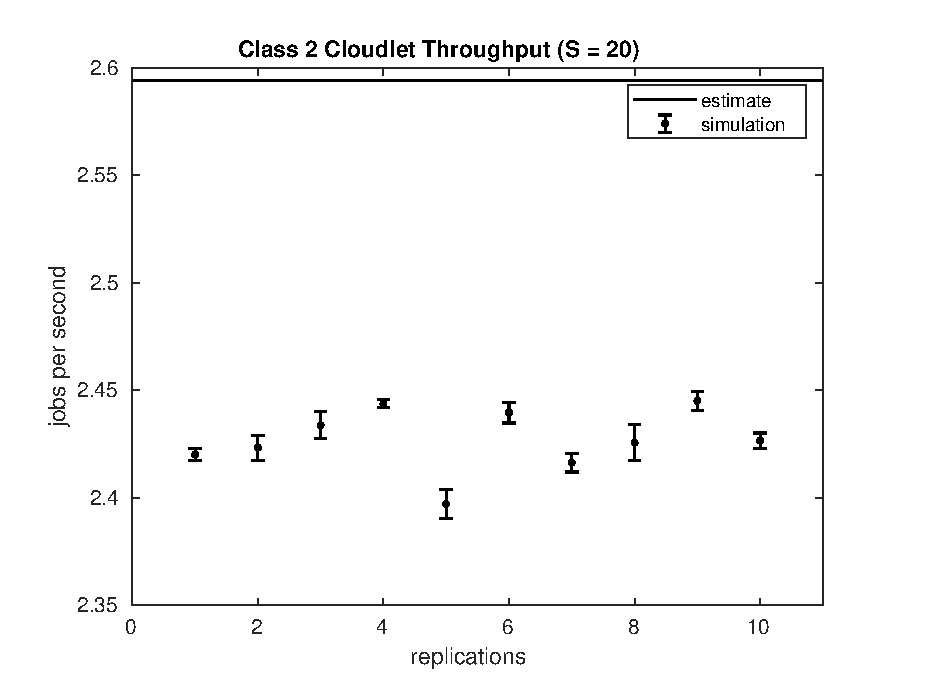
\includegraphics[width=\textwidth]{figures/simul/20_500K_x2clet}
\caption{$S = 20$}
\label{20_x2clet}
\end{subfigure}
%
\begin{subfigure}[t]{0.49\textwidth}
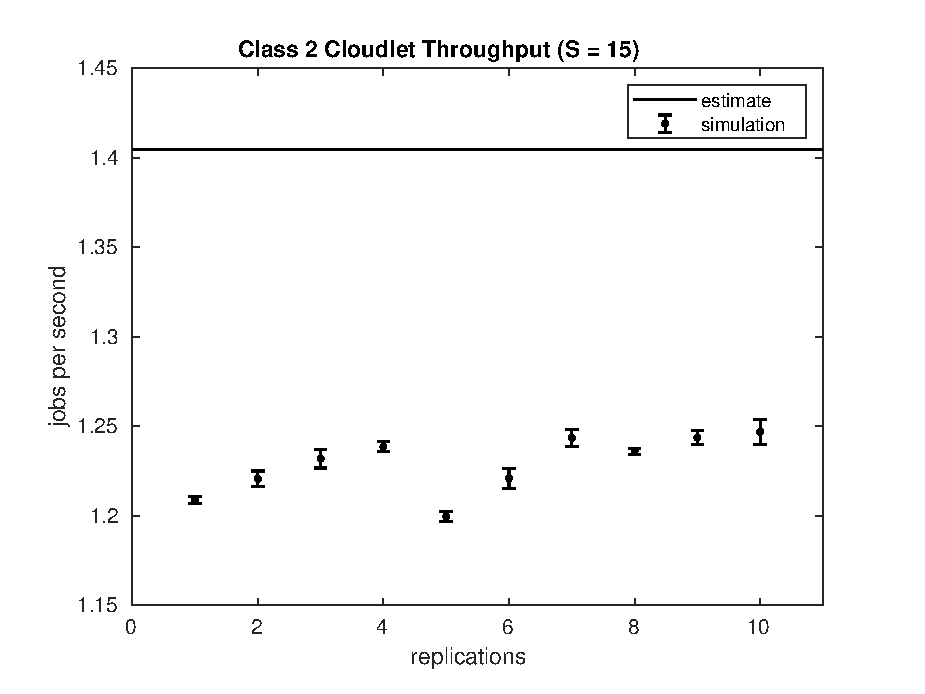
\includegraphics[width=\textwidth]{figures/simul/15_500K_x2clet}
\caption{$S = 15$}
\label{15_x2clet}
\end{subfigure}
%
\begin{subfigure}[t]{0.49\textwidth}
\includegraphics[width=\textwidth]{figures/simul/10_500K_x2clet}
\caption{$S = 10$}
\label{10_x2clet}
\end{subfigure}
%
\begin{subfigure}[t]{0.49\textwidth}
\includegraphics[width=\textwidth]{figures/simul/5_500K_x2clet}
\caption{$S = 5$}
\label{5_x2clet}
\end{subfigure}
%
\caption{throughput cloudlet classe 2}
\label{plot:x2clet}
\end{figure}
%
%
\begin{table}[!h]
\begin{adjustbox}{width=\textwidth}
\begin{tabular}{c|r@{.}l|r@{.}l|r@{.}l|r@{.}l}
& \multicolumn{2}{|c|}{$S=20$}
& \multicolumn{2}{|c|}{$S=15$}
& \multicolumn{2}{|c|}{$S=10$}
& \multicolumn{2}{|c}{$S=5$}
\\          
\hline
R1      & $2$&$4201 \pm 0.0027$ & $1$&$2090 \pm 0.0019$ & $0$&$3054 \pm 0.0013$ & $0$&$0132 \pm 0.0003$ \\
R2      & $2$&$4234 \pm 0.0058$ & $1$&$2207 \pm 0.0043$ & $0$&$3145 \pm 0.0013$ & $0$&$0142 \pm 0.0003$ \\
R3      & $2$&$4338 \pm 0.0064$ & $1$&$2320 \pm 0.0053$ & $0$&$3052 \pm 0.0011$ & $0$&$0118 \pm 0.0005$ \\
R4      & $2$&$4438 \pm 0.0019$ & $1$&$2387 \pm 0.0030$ & $0$&$3171 \pm 0.0009$ & $0$&$0141 \pm 0.0004$ \\
R5      & $2$&$3972 \pm 0.0066$ & $1$&$1996 \pm 0.0026$ & $0$&$3063 \pm 0.0014$ & $0$&$0137 \pm 0.0004$ \\
R6      & $2$&$4397 \pm 0.0048$ & $1$&$2209 \pm 0.0056$ & $0$&$3074 \pm 0.0033$ & $0$&$0137 \pm 0.0004$ \\
R7      & $2$&$4164 \pm 0.0044$ & $1$&$2436 \pm 0.0047$ & $0$&$3029 \pm 0.0025$ & $0$&$0133 \pm 0.0008$ \\
R8      & $2$&$4257 \pm 0.0084$ & $1$&$2360 \pm 0.0017$ & $0$&$3153 \pm 0.0012$ & $0$&$0127 \pm 0.0003$ \\
R9      & $2$&$4452 \pm 0.0044$ & $1$&$2436 \pm 0.0038$ & $0$&$3192 \pm 0.0018$ & $0$&$0152 \pm 0.0009$ \\
R10     & $2$&$4267 \pm 0.0035$ & $1$&$2469 \pm 0.0070$ & $0$&$3248 \pm 0.0034$ & $0$&$0145 \pm 0.0003$ \\
EST     & $2$&$5943$            & $1$&$4046$            & $0$&$3880$            & $0$&$0165$            \\
\epsmx  & $0$&$1905 \ (7.9\%)$  & $0$&$2024 \ (16.9\%)$ & $0$&$0826 \ (27.3\%)$ & $0$&$0042 \ (36.0\%)$   
\end{tabular}
\end{adjustbox}
\caption{throughput cloudlet classe 2}
\label{tab:x2clet}
\end{table}

%%%%%%%%%%%%%%%%%%%%%%%%%%%%%%%%%%%%%%%%%%%%%%%%%%%%%%%%%%%%%%%%%%%%%%%%%%%%%%%%
\subsection{Throughput Cloudlet}
La figura~\ref{plot:xclet} e la tabella~\ref{tab:xclet} mostrano che l'errore
di approssimazione dovuto alla percentuale di job interrotti viene attenuato.
Tale attenuazione risulta tanto più maggiore quanto lo è la probabilità di
interruzione, poiché ogni interruzione implica un completamento in più di classe
1, che andrà ad influire sul calcolo del throughput.

L'andamento è sempre proporzionale ad $S$ e la stima della statistica è
affidabile con un errore massimo che va dal $2\%$ al $4\%$ nei casi in cui
$S=10,15,20$, altrimenti nel caso in cui $S=5$ l'errore
massimo è inferiore all'$1\%$.
\begin{figure}[!h]
\centering
%
\begin{subfigure}[t]{0.49\textwidth}
\includegraphics[width=\textwidth]{figures/simul/20_500K_xclet}
\caption{$S = 20$}
\label{20_xclet}
\end{subfigure}
%
\begin{subfigure}[t]{0.49\textwidth}
\includegraphics[width=\textwidth]{figures/simul/15_500K_xclet}
\caption{$S = 15$}
\label{15_xclet}
\end{subfigure}
%
\begin{subfigure}[t]{0.49\textwidth}
\includegraphics[width=\textwidth]{figures/simul/10_500K_xclet}
\caption{$S = 10$}
\label{10_xclet}
\end{subfigure}
%
\begin{subfigure}[t]{0.49\textwidth}
\includegraphics[width=\textwidth]{figures/simul/5_500K_xclet}
\caption{$S = 5$}
\label{5_xclet}
\end{subfigure}
%
\caption{throughput cloudlet}
\label{plot:xclet}
\end{figure}
%
%
\begin{table}[!h]
\begin{adjustbox}{width=\textwidth}
\begin{tabular}{c|r@{.}l|r@{.}l|r@{.}l|r@{.}l}
& \multicolumn{2}{|c|}{$S=20$}
& \multicolumn{2}{|c|}{$S=15$}
& \multicolumn{2}{|c|}{$S=10$}
& \multicolumn{2}{|c}{$S=5$}
\\          
\hline
R1      & $6$&$4255 \pm 0.0042$ & $5$&$2144 \pm 0.0047$ & $4$&$3108 \pm 0.0047$ & $4$&$0185 \pm 0.0041$ \\
R2      & $6$&$4255 \pm 0.0030$ & $5$&$2254 \pm 0.0028$ & $4$&$3185 \pm 0.0030$ & $4$&$0179 \pm 0.0040$ \\
R3      & $6$&$4510 \pm 0.0057$ & $5$&$2463 \pm 0.0037$ & $4$&$3204 \pm 0.0030$ & $4$&$0280 \pm 0.0026$ \\
R4      & $6$&$4207 \pm 0.0036$ & $5$&$2228 \pm 0.0013$ & $4$&$2954 \pm 0.0033$ & $3$&$9881 \pm 0.0062$ \\
R5      & $6$&$4219 \pm 0.0057$ & $5$&$2071 \pm 0.0028$ & $4$&$3302 \pm 0.0032$ & $4$&$0373 \pm 0.0032$ \\
R6      & $6$&$4412 \pm 0.0043$ & $5$&$2138 \pm 0.0023$ & $4$&$2997 \pm 0.0043$ & $4$&$0044 \pm 0.0066$ \\
R7      & $6$&$4387 \pm 0.0041$ & $5$&$2242 \pm 0.0023$ & $4$&$3089 \pm 0.0064$ & $4$&$0211 \pm 0.0058$ \\
R8      & $6$&$4193 \pm 0.0033$ & $5$&$2277 \pm 0.0019$ & $4$&$3096 \pm 0.0041$ & $4$&$0186 \pm 0.0035$ \\
R9      & $6$&$4276 \pm 0.0050$ & $5$&$2300 \pm 0.0050$ & $4$&$3028 \pm 0.0041$ & $3$&$9958 \pm 0.0051$ \\
R10     & $6$&$4272 \pm 0.0021$ & $5$&$2336 \pm 0.0038$ & $4$&$3143 \pm 0.0022$ & $4$&$0019 \pm 0.0046$ \\
EST     & $6$&$5922$            & $5$&$4025$            & $4$&$3858$            & $4$&$0144$            \\
\epsmx  & $0$&$1696 \ (2.6\%)$  & $0$&$1926 \ (3.7\%)$  & $0$&$0872 \ (2.0\%)$  & $0$&$0261 \ (0.6\%)$    
\end{tabular}
\end{adjustbox}
\caption{throughput cloudlet}
\label{tab:xclet}
\end{table}

%%%%%%%%%%%%%%%%%%%%%%%%%%%%%%%%%%%%%%%%%%%%%%%%%%%%%%%%%%%%%%%%%%%%%%%%%%%%%%%%
\subsection{Throughput Sistema}
Le figure~\ref{plot:x1},~\ref{plot:x2} e~\ref{plot:x} e la
tabelle~\ref{tab:x1},~\ref{tab:x2} e~\ref{tab:x} mostrano i risultati relativi
al throughput del sistema sia per classe che globalmente in cui viene confermata
l'ipotesi di stabilità sfruttata nel modello analitico, infatti risulta che i
valori del throughput sono indipendenti dal parametro $S$ ed equivalgono ai
relativi tassi di ingresso. 

Le stime approssimano bene i valori delle simulazioni con un errore massimo
inferiore all'$1\%$.
\begin{figure}[!h]
\centering
%
\begin{subfigure}[t]{0.49\textwidth}
\includegraphics[width=\textwidth]{figures/simul/20_500K_x1}
\caption{$S = 20$}
\label{20_x1}
\end{subfigure}
%
\begin{subfigure}[t]{0.49\textwidth}
\includegraphics[width=\textwidth]{figures/simul/15_500K_x1}
\caption{$S = 15$}
\label{15_x1}
\end{subfigure}
%
\begin{subfigure}[t]{0.49\textwidth}
\includegraphics[width=\textwidth]{figures/simul/10_500K_x1}
\caption{$S = 10$}
\label{10_x1}
\end{subfigure}
%
\begin{subfigure}[t]{0.49\textwidth}
\includegraphics[width=\textwidth]{figures/simul/5_500K_x1}
\caption{$S = 5$}
\label{5_x1}
\end{subfigure}
%
\caption{throughput sistema classe 1}
\label{plot:x1}
\end{figure}
%
%
\begin{table}[!h]
\begin{adjustbox}{width=\textwidth}
\begin{tabular}{c|r@{.}l|r@{.}l|r@{.}l|r@{.}l}
& \multicolumn{2}{|c|}{$S=20$}
& \multicolumn{2}{|c|}{$S=15$}
& \multicolumn{2}{|c|}{$S=10$}
& \multicolumn{2}{|c}{$S=5$}
\\          
\hline
R1      & $4$&$0067 \pm 0.0044$ & $4$&$0067 \pm 0.0043$ & $4$&$0067 \pm 0.0044$ & $4$&$0067 \pm 0.0044$ \\
R2      & $4$&$0056 \pm 0.0050$ & $4$&$0082 \pm 0.0044$ & $4$&$0076 \pm 0.0044$ & $4$&$0072 \pm 0.0044$ \\
R3      & $4$&$0187 \pm 0.0021$ & $4$&$0158 \pm 0.0041$ & $4$&$0167 \pm 0.0033$ & $4$&$0178 \pm 0.0024$ \\
R4      & $3$&$9789 \pm 0.0044$ & $3$&$9865 \pm 0.0032$ & $3$&$9803 \pm 0.0037$ & $3$&$9761 \pm 0.0065$ \\
R5      & $4$&$0268 \pm 0.0027$ & $4$&$0095 \pm 0.0022$ & $4$&$0260 \pm 0.0028$ & $4$&$0257 \pm 0.0029$ \\
R6      & $4$&$0035 \pm 0.0022$ & $3$&$9947 \pm 0.0048$ & $3$&$9942 \pm 0.0065$ & $3$&$9925 \pm 0.0071$ \\
R7      & $4$&$0246 \pm 0.0073$ & $3$&$9830 \pm 0.0059$ & $4$&$0084 \pm 0.0084$ & $4$&$0109 \pm 0.0059$ \\
R8      & $3$&$9964 \pm 0.0109$ & $3$&$9941 \pm 0.0023$ & $3$&$9967 \pm 0.0037$ & $4$&$0089 \pm 0.0036$ \\
R9      & $3$&$9844 \pm 0.0032$ & $3$&$9885 \pm 0.0028$ & $3$&$9852 \pm 0.0032$ & $3$&$9827 \pm 0.0059$ \\
R10     & $4$&$0034 \pm 0.0034$ & $3$&$9887 \pm 0.0051$ & $3$&$9916 \pm 0.0042$ & $3$&$9894 \pm 0.0046$ \\
EST     & $4$&$0000$            & $4$&$0000$            & $4$&$0000$            & $4$&$0000$            \\
\epsmx  & $0$&$0319 \ (0.8\%)$  & $0$&$0199 \ (0.5\%)$  & $0$&$0288 \ (0.7\%)$  & $0$&$0286 \ (0.7\%)$    
\end{tabular}
\end{adjustbox}
\caption{throughput sistema classe 1}
\label{tab:x1}
\end{table}

%%%%%%%%%%%%%%%%%%%%%%%%%%%%%%%%%%%%%%%%%%%%%%%%%%%%%%%%%%%%%%%%%%%%%%%%%%%%%%%%
\begin{figure}[!h]
\centering
%
\begin{subfigure}[t]{0.49\textwidth}
\includegraphics[width=\textwidth]{figures/simul/20_500K_x2}
\caption{$S = 20$}
\label{20_x2}
\end{subfigure}
%
\begin{subfigure}[t]{0.49\textwidth}
\includegraphics[width=\textwidth]{figures/simul/15_500K_x2}
\caption{$S = 15$}
\label{15_x2}
\end{subfigure}
%
\begin{subfigure}[t]{0.49\textwidth}
\includegraphics[width=\textwidth]{figures/simul/10_500K_x2}
\caption{$S = 10$}
\label{10_x2}
\end{subfigure}
%
\begin{subfigure}[t]{0.49\textwidth}
\includegraphics[width=\textwidth]{figures/simul/5_500K_x2}
\caption{$S = 5$}
\label{5_x2}
\end{subfigure}
%
\caption{throughput sistema classe 2}
\label{plot:x2}
\end{figure}
%
%
\begin{table}[!h]
\begin{adjustbox}{width=\textwidth}
\begin{tabular}{c|r@{.}l|r@{.}l|r@{.}l|r@{.}l}
& \multicolumn{2}{|c|}{$S=20$}
& \multicolumn{2}{|c|}{$S=15$}
& \multicolumn{2}{|c|}{$S=10$}
& \multicolumn{2}{|c}{$S=5$}
\\          
\hline
R1      & $6$&$2431 \pm 0.0101$ & $6$&$2428 \pm 0.0103$ & $6$&$2429 \pm 0.0103$ & $6$&$2430 \pm 0.0102$ \\
R2      & $6$&$2230 \pm 0.0072$ & $6$&$2229 \pm 0.0076$ & $6$&$2231 \pm 0.0074$ & $6$&$2232 \pm 0.0074$ \\
R3      & $6$&$2559 \pm 0.0083$ & $6$&$2556 \pm 0.0084$ & $6$&$2556 \pm 0.0085$ & $6$&$2557 \pm 0.0084$ \\
R4      & $6$&$2282 \pm 0.0068$ & $6$&$2366 \pm 0.0088$ & $6$&$2274 \pm 0.0076$ & $6$&$2314 \pm 0.0042$ \\
R5      & $6$&$2075 \pm 0.0044$ & $6$&$2562 \pm 0.0092$ & $6$&$2053 \pm 0.0063$ & $6$&$2051 \pm 0.0063$ \\
R6      & $6$&$2481 \pm 0.0048$ & $6$&$2355 \pm 0.0115$ & $6$&$2381 \pm 0.0109$ & $6$&$2373 \pm 0.0114$ \\
R7      & $6$&$2753 \pm 0.0061$ & $6$&$2301 \pm 0.0117$ & $6$&$2683 \pm 0.0027$ & $6$&$2725 \pm 0.0032$ \\
R8      & $6$&$2661 \pm 0.0055$ & $6$&$2477 \pm 0.0023$ & $6$&$2461 \pm 0.0029$ & $6$&$2623 \pm 0.0054$ \\
R9      & $6$&$2387 \pm 0.0061$ & $6$&$2753 \pm 0.0060$ & $6$&$2744 \pm 0.0066$ & $6$&$2755 \pm 0.0065$ \\
R10     & $6$&$2370 \pm 0.0029$ & $6$&$2272 \pm 0.0104$ & $6$&$2276 \pm 0.0105$ & $6$&$2261 \pm 0.0108$ \\
EST     & $6$&$2500$            & $6$&$2500$            & $6$&$2500$            & $6$&$2500$            \\
\epsmx  & $0$&$0381 \ (0.6\%)$  & $0$&$0313 \ (0.5\%)$  & $0$&$0384 \ (0.6\%)$  & $0$&$0386 \ (0.6\%)$    
\end{tabular}
\end{adjustbox}
\caption{throughput sistema classe 2}
\label{tab:x2}
\end{table}

%%%%%%%%%%%%%%%%%%%%%%%%%%%%%%%%%%%%%%%%%%%%%%%%%%%%%%%%%%%%%%%%%%%%%%%%%%%%%%%%
\begin{figure}[!h]
\centering
%
\begin{subfigure}[t]{0.49\textwidth}
\includegraphics[width=\textwidth]{figures/simul/20_500K_x}
\caption{$S = 20$}
\label{20_x}
\end{subfigure}
%
\begin{subfigure}[t]{0.49\textwidth}
\includegraphics[width=\textwidth]{figures/simul/15_500K_x}
\caption{$S = 15$}
\label{15_x}
\end{subfigure}
%
\begin{subfigure}[t]{0.49\textwidth}
\includegraphics[width=\textwidth]{figures/simul/10_500K_x}
\caption{$S = 10$}
\label{10_x}
\end{subfigure}
%
\begin{subfigure}[t]{0.49\textwidth}
\includegraphics[width=\textwidth]{figures/simul/5_500K_x}
\caption{$S = 5$}
\label{5_x}
\end{subfigure}
%
\caption{throughput sistema}
\label{plot:x}
\end{figure}
%
%
\begin{table}[!h]
\begin{adjustbox}{width=\textwidth}
\begin{tabular}{c|r@{.}l|r@{.}l|r@{.}l|r@{.}l}
& \multicolumn{2}{|c|}{$S=20$}
& \multicolumn{2}{|c|}{$S=15$}
& \multicolumn{2}{|c|}{$S=10$}
& \multicolumn{2}{|c}{$S=5$}
\\          
\hline
R1      & $10$&$2498 \pm 0.0138$ & $10$&$2496 \pm 0.0140$ & $10$&$2496 \pm 0.0140$ & $10$&$2497 \pm 0.0139$ \\
R2      & $10$&$2286 \pm 0.0076$ & $10$&$2311 \pm 0.0056$ & $10$&$2306 \pm 0.0060$ & $10$&$2303 \pm 0.0062$ \\
R3      & $10$&$2746 \pm 0.0088$ & $10$&$2714 \pm 0.0116$ & $10$&$2723 \pm 0.0108$ & $10$&$2734 \pm 0.0095$ \\
R4      & $10$&$2071 \pm 0.0102$ & $10$&$2231 \pm 0.0105$ & $10$&$2077 \pm 0.0096$ & $10$&$2075 \pm 0.0098$ \\
R5      & $10$&$2343 \pm 0.0042$ & $10$&$2656 \pm 0.0105$ & $10$&$2313 \pm 0.0069$ & $10$&$2308 \pm 0.0072$ \\
R6      & $10$&$2516 \pm 0.0039$ & $10$&$2302 \pm 0.0154$ & $10$&$2323 \pm 0.0168$ & $10$&$2298 \pm 0.0180$ \\
R7      & $10$&$2999 \pm 0.0086$ & $10$&$2132 \pm 0.0174$ & $10$&$2766 \pm 0.0097$ & $10$&$2834 \pm 0.0048$ \\
R8      & $10$&$2625 \pm 0.0117$ & $10$&$2418 \pm 0.0033$ & $10$&$2428 \pm 0.0037$ & $10$&$2712 \pm 0.0071$ \\
R9      & $10$&$2231 \pm 0.0085$ & $10$&$2638 \pm 0.0072$ & $10$&$2596 \pm 0.0090$ & $10$&$2582 \pm 0.0116$ \\
R10     & $10$&$2404 \pm 0.0038$ & $10$&$2160 \pm 0.0143$ & $10$&$2192 \pm 0.0121$ & $10$&$2156 \pm 0.0142$ \\
EST     & $10$&$2500$            & $10$&$2500$            & $10$&$2500$            & $10$&$2500$            \\
\epsmx  & $0$&$0584 \ (0.6\%)$   & $0$&$0330 \ (0.3\%)$   & $0$&$0363 \ (0.4\%)$   & $0$&$0382 \ (0.4\%)$     
\end{tabular}
\end{adjustbox}
\caption{throughput sistema}
\label{tab:x}
\end{table}

%%%%%%%%%%%%%%%%%%%%%%%%%%%%%%%%%%%%%%%%%%%%%%%%%%%%%%%%%%%%%%%%%%%%%%%%%%%%%%%%
\subsection{Popolazione Cloudlet Classe 1}
La figura~\ref{plot:n1clet} e la tabella~\ref{tab:n1clet} mostrano che i valori
della popolazione media per i job di classe nel cloudlet sono pressoché costanti
al variare del parametro $S$, a causa della bassa probabilità che un job di
classe 1 venga inviato al server remoto. La stima approssima bene i risultati
con un errore massimo pari all'$1\%$.
\begin{figure}[!h]
\centering
%
\begin{subfigure}[t]{0.49\textwidth}
\includegraphics[width=\textwidth]{figures/simul/20_500K_n1clet}
\caption{$S = 20$}
\label{20_n1clet}
\end{subfigure}
%
\begin{subfigure}[t]{0.49\textwidth}
\includegraphics[width=\textwidth]{figures/simul/15_500K_n1clet}
\caption{$S = 15$}
\label{15_n1clet}
\end{subfigure}
%
\begin{subfigure}[t]{0.49\textwidth}
\includegraphics[width=\textwidth]{figures/simul/10_500K_n1clet}
\caption{$S = 10$}
\label{10_n1clet}
\end{subfigure}
%
\begin{subfigure}[t]{0.49\textwidth}
\includegraphics[width=\textwidth]{figures/simul/5_500K_n1clet}
\caption{$S = 5$}
\label{5_n1clet}
\end{subfigure}
%
\caption{popolazione cloudlet classe 1}
\label{plot:n1clet}
\end{figure}
%
%
\begin{table}[!h]
\begin{adjustbox}{width=\textwidth}
\begin{tabular}{c|r@{.}l|r@{.}l|r@{.}l|r@{.}l}
& \multicolumn{2}{|c|}{$S=20$}
& \multicolumn{2}{|c|}{$S=15$}
& \multicolumn{2}{|c|}{$S=10$}
& \multicolumn{2}{|c}{$S=5$}
\\          
\hline
R1      & $8$&$9175 \pm 0.0070$ & $8$&$9175 \pm 0.0070$ & $8$&$9175 \pm 0.0070$ & $8$&$9175 \pm 0.0070$ \\
R2      & $8$&$8757 \pm 0.0154$ & $8$&$8834 \pm 0.0158$ & $8$&$8801 \pm 0.0152$ & $8$&$8783 \pm 0.0152$ \\
R3      & $8$&$9431 \pm 0.0074$ & $8$&$9370 \pm 0.0124$ & $8$&$9380 \pm 0.0115$ & $8$&$9399 \pm 0.0095$ \\
R4      & $8$&$8371 \pm 0.0222$ & $8$&$8193 \pm 0.0098$ & $8$&$8389 \pm 0.0202$ & $8$&$8367 \pm 0.0212$ \\
R5      & $8$&$9625 \pm 0.0149$ & $8$&$9151 \pm 0.0082$ & $8$&$9575 \pm 0.0109$ & $8$&$9462 \pm 0.0100$ \\
R6      & $8$&$8553 \pm 0.0072$ & $8$&$8850 \pm 0.0185$ & $8$&$8816 \pm 0.0205$ & $8$&$8722 \pm 0.0232$ \\
R7      & $8$&$9466 \pm 0.0131$ & $8$&$7982 \pm 0.0242$ & $8$&$9220 \pm 0.0190$ & $8$&$9277 \pm 0.0165$ \\
R8      & $8$&$8924 \pm 0.0302$ & $8$&$8328 \pm 0.0074$ & $8$&$8451 \pm 0.0088$ & $8$&$9244 \pm 0.0106$ \\
R9      & $8$&$8399 \pm 0.0127$ & $8$&$8353 \pm 0.0060$ & $8$&$8301 \pm 0.0065$ & $8$&$8258 \pm 0.0122$ \\
R10     & $8$&$8683 \pm 0.0112$ & $8$&$7973 \pm 0.0210$ & $8$&$8036 \pm 0.0176$ & $8$&$7986 \pm 0.0187$ \\
EST     & $8$&$8841$            & $8$&$8841$            & $8$&$8841$            & $8$&$8841$            \\
\epsmx  & $0$&$0933 \ (1.0\%)$  & $0$&$0659 \ (0.7\%)$  & $0$&$0842 \ (0.9\%)$  & $0$&$0721 \ (0.8\%)$    
\end{tabular}
\end{adjustbox}
\caption{popolazione cloudlet classe 1}
\label{tab:n1clet}
\end{table}

%%%%%%%%%%%%%%%%%%%%%%%%%%%%%%%%%%%%%%%%%%%%%%%%%%%%%%%%%%%%%%%%%%%%%%%%%%%%%%%%
\subsection{Popolazione Cloudlet Classe 2}
La figura~\ref{plot:n2clet} e la tabella~\ref{tab:n2clet} mostrano che la
popolazione media dei job di classe 2 diminuisce al decrescere del parametro
$S$, ciò è lecito poiché con l'abbassamento del valore di soglia vengono
accettati sempre meno job di classe 2.

La stima commette un'errore che invece aumenta al decrescere di $S$,
probabilmente dovuto a inprecisioni della distribuzione stazionaria, che saranno
anche la causa del valore approssimato della percentuale di interruzione.
\begin{figure}[!h]
\centering
%
\begin{subfigure}[t]{0.49\textwidth}
\includegraphics[width=\textwidth]{figures/simul/20_500K_n2clet}
\caption{$S = 20$}
\label{20_n2clet}
\end{subfigure}
%
\begin{subfigure}[t]{0.49\textwidth}
\includegraphics[width=\textwidth]{figures/simul/15_500K_n2clet}
\caption{$S = 15$}
\label{15_n2clet}
\end{subfigure}
%
\begin{subfigure}[t]{0.49\textwidth}
\includegraphics[width=\textwidth]{figures/simul/10_500K_n2clet}
\caption{$S = 10$}
\label{10_n2clet}
\end{subfigure}
%
\begin{subfigure}[t]{0.49\textwidth}
\includegraphics[width=\textwidth]{figures/simul/5_500K_n2clet}
\caption{$S = 5$}
\label{5_n2clet}
\end{subfigure}
%
\caption{popolazione cloudlet classe 2}
\label{plot:n2clet}
\end{figure}
%
%
\begin{table}[!h]
\begin{adjustbox}{width=\textwidth}
\begin{tabular}{c|r@{.}l|r@{.}l|r@{.}l|r@{.}l}
& \multicolumn{2}{|c|}{$S=20$}
& \multicolumn{2}{|c|}{$S=15$}
& \multicolumn{2}{|c|}{$S=10$}
& \multicolumn{2}{|c}{$S=5$}
\\          
\hline
R1      & $9$&$6707 \pm 0.0069$ & $5$&$2295 \pm 0.0069$ & $1$&$4243 \pm 0.0045$ & $0$&$0613 \pm 0.0011$ \\
R2      & $9$&$6856 \pm 0.0183$ & $5$&$2579 \pm 0.0164$ & $1$&$4540 \pm 0.0095$ & $0$&$0652 \pm 0.0015$ \\
R3      & $9$&$6394 \pm 0.0059$ & $5$&$2088 \pm 0.0076$ & $1$&$3996 \pm 0.0042$ & $0$&$0558 \pm 0.0007$ \\
R4      & $9$&$7394 \pm 0.0208$ & $5$&$3249 \pm 0.0077$ & $1$&$4784 \pm 0.0068$ & $0$&$0638 \pm 0.0014$ \\
R5      & $9$&$6128 \pm 0.0188$ & $5$&$2324 \pm 0.0070$ & $1$&$4243 \pm 0.0041$ & $0$&$0637 \pm 0.0008$ \\
R6      & $9$&$7140 \pm 0.0089$ & $5$&$2611 \pm 0.0164$ & $1$&$4530 \pm 0.0106$ & $0$&$0605 \pm 0.0018$ \\
R7      & $9$&$6312 \pm 0.0120$ & $5$&$3423 \pm 0.0192$ & $1$&$4291 \pm 0.0097$ & $0$&$0587 \pm 0.0014$ \\
R8      & $9$&$6854 \pm 0.0230$ & $5$&$3087 \pm 0.0054$ & $1$&$4778 \pm 0.0062$ & $0$&$0594 \pm 0.0010$ \\
R9      & $9$&$7243 \pm 0.0092$ & $5$&$3002 \pm 0.0068$ & $1$&$4780 \pm 0.0039$ & $0$&$0662 \pm 0.0018$ \\
R10     & $9$&$7099 \pm 0.0093$ & $5$&$3322 \pm 0.0171$ & $1$&$4895 \pm 0.0111$ & $0$&$0669 \pm 0.0012$ \\
EST     & $9$&$6087$            & $5$&$2024$            & $1$&$4370$            & $0$&$0611$            \\
\epsmx  & $0$&$1515 \ (1.6\%)$  & $0$&$1592 \ (3.0\%)$  & $0$&$0637 \ (4.3\%)$  & $0$&$0069 \ (10.3\%)$   
\end{tabular}
\end{adjustbox}
\caption{popolazione cloudlet classe 2}
\label{tab:n2clet}
\end{table}

%%%%%%%%%%%%%%%%%%%%%%%%%%%%%%%%%%%%%%%%%%%%%%%%%%%%%%%%%%%%%%%%%%%%%%%%%%%%%%%%
\subsection{Popolazione Cloud Classe 1}
La figura~\ref{plot:n1cloud} e la tabella~\ref{tab:n1cloud} mostrano la
popolazione media del cloudlet relativa ai job di classe 1 prossima allo 0, per
il solito motivo della remota probabilità di blocco.

Il numero di job è talmente basso, che ogni replica della simulazione può
produrre risultati molto variegati, infatti vengono prodotti intarvalli di
confidenza ampi e la stima del modello analitico può commettere un errore anche
del $65\%$.
\begin{figure}[!h]
\centering
%
\begin{subfigure}[t]{0.49\textwidth}
\includegraphics[width=\textwidth]{figures/simul/20_500K_n1cloud}
\caption{$S = 20$}
\label{20_n1cloud}
\end{subfigure}
%
\begin{subfigure}[t]{0.49\textwidth}
\includegraphics[width=\textwidth]{figures/simul/15_500K_n1cloud}
\caption{$S = 15$}
\label{15_n1cloud}
\end{subfigure}
%
\begin{subfigure}[t]{0.49\textwidth}
\includegraphics[width=\textwidth]{figures/simul/10_500K_n1cloud}
\caption{$S = 10$}
\label{10_n1cloud}
\end{subfigure}
%
\begin{subfigure}[t]{0.49\textwidth}
\includegraphics[width=\textwidth]{figures/simul/5_500K_n1cloud}
\caption{$S = 5$}
\label{5_n1cloud}
\end{subfigure}
%
\caption{popolazione cloud classe 1}
\label{plot:n1cloud}
\end{figure}
%
%
\begin{table}[!h]
\begin{adjustbox}{width=\textwidth}
\begin{tabular}{c|r@{.}l|r@{.}l|r@{.}l|r@{.}l}
& \multicolumn{2}{|c|}{$S=20$}
& \multicolumn{2}{|c|}{$S=15$}
& \multicolumn{2}{|c|}{$S=10$}
& \multicolumn{2}{|c}{$S=5$}
\\          
\hline
R1      & $0$&$0049 \pm 0.0004$ & $0$&$0049 \pm 0.0004$ & $0$&$0049 \pm 0.0004$ & $0$&$0049 \pm 0.0004$ \\
R2      & $0$&$0183 \pm 0.0024$ & $0$&$0164 \pm 0.0019$ & $0$&$0170 \pm 0.0019$ & $0$&$0143 \pm 0.0017$ \\
R3      & $0$&$0063 \pm 0.0005$ & $0$&$0052 \pm 0.0004$ & $0$&$0053 \pm 0.0004$ & $0$&$0062 \pm 0.0004$ \\
R4      & $0$&$0097 \pm 0.0005$ & $0$&$0103 \pm 0.0007$ & $0$&$0084 \pm 0.0008$ & $0$&$0079 \pm 0.0007$ \\
R5      & $0$&$0076 \pm 0.0003$ & $0$&$0063 \pm 0.0006$ & $0$&$0088 \pm 0.0006$ & $0$&$0074 \pm 0.0005$ \\
R6      & $0$&$0079 \pm 0.0004$ & $0$&$0064 \pm 0.0003$ & $0$&$0067 \pm 0.0003$ & $0$&$0061 \pm 0.0003$ \\
R7      & $0$&$0113 \pm 0.0006$ & $0$&$0070 \pm 0.0005$ & $0$&$0099 \pm 0.0005$ & $0$&$0109 \pm 0.0016$ \\
R8      & $0$&$0125 \pm 0.0007$ & $0$&$0082 \pm 0.0005$ & $0$&$0086 \pm 0.0005$ & $0$&$0124 \pm 0.0006$ \\
R9      & $0$&$0061 \pm 0.0005$ & $0$&$0062 \pm 0.0002$ & $0$&$0060 \pm 0.0005$ & $0$&$0087 \pm 0.0007$ \\
R10     & $0$&$0126 \pm 0.0006$ & $0$&$0074 \pm 0.0005$ & $0$&$0073 \pm 0.0003$ & $0$&$0078 \pm 0.0005$ \\
EST     & $0$&$0086$            & $0$&$0086$            & $0$&$0086$            & $0$&$0086$            \\
\epsmx  & $0$&$0121 \ (65.9\%)$ & $0$&$0098 \ (59.3\%)$ & $0$&$0103 \ (60.5\%)$ & $0$&$0074 \ (51.9\%)$   
\end{tabular}
\end{adjustbox}
\caption{popolazione cloud classe 1}
\label{tab:n1cloud}
\end{table}

%%%%%%%%%%%%%%%%%%%%%%%%%%%%%%%%%%%%%%%%%%%%%%%%%%%%%%%%%%%%%%%%%%%%%%%%%%%%%%%%
\subsection{Popolazione Cloud Classe 2}
La popolazione media del cloud relativa ai job di classe 2 varia in maniera
opposta alla popolazione media del cloudlet, infatti cresce all'aumentare della
probabilità di interruzione. 

La figura~\ref{plot:n2cloud} e la tabella~\ref{tab:n2cloud} mostrano i risultati
delle simulazioni a confronto con le stime del modello analitico e, anche per
quanto riguarda l'errore massimo, si ha un andamento inverso a quello relativo
al cloudlet, infatti l'errore massimo aumenta al crescere di $S$. Inoltre, nei
casi in cui $S=10,15,20$, la stima è leggermente inferiore ai risultati poiché
il tasso di arrivo al nodo è proporzionale alla percentuale di interruzione,
pertanto anche in questo caso ci si porta dietro l'errore di approssimazione.
\begin{figure}[!h]
\centering
%
\begin{subfigure}[t]{0.49\textwidth}
\includegraphics[width=\textwidth]{figures/simul/20_500K_n2cloud}
\caption{$S = 20$}
\label{20_n2cloud}
\end{subfigure}
%
\begin{subfigure}[t]{0.49\textwidth}
\includegraphics[width=\textwidth]{figures/simul/15_500K_n2cloud}
\caption{$S = 15$}
\label{15_n2cloud}
\end{subfigure}
%
\begin{subfigure}[t]{0.49\textwidth}
\includegraphics[width=\textwidth]{figures/simul/10_500K_n2cloud}
\caption{$S = 10$}
\label{10_n2cloud}
\end{subfigure}
%
\begin{subfigure}[t]{0.49\textwidth}
\includegraphics[width=\textwidth]{figures/simul/5_500K_n2cloud}
\caption{$S = 5$}
\label{5_n2cloud}
\end{subfigure}
%
\caption{popolazione cloud classe 2}
\label{plot:n2cloud}
\end{figure}
%
%
\begin{table}[!h]
\begin{adjustbox}{width=\textwidth}
\begin{tabular}{c|r@{.}l|r@{.}l|r@{.}l|r@{.}l}
& \multicolumn{2}{|c|}{$S=20$}
& \multicolumn{2}{|c|}{$S=15$}
& \multicolumn{2}{|c|}{$S=10$}
& \multicolumn{2}{|c}{$S=5$}
\\          
\hline
R1      & $17$&$3911 \pm 0.0508$ & $22$&$8912 \pm 0.0481$ & $26$&$9995 \pm 0.0462$ & $28$&$3291 \pm 0.0487$ \\
R2      & $17$&$3631 \pm 0.0287$ & $22$&$8482 \pm 0.0162$ & $26$&$9781 \pm 0.0227$ & $28$&$3499 \pm 0.0253$ \\
R3      & $17$&$4461 \pm 0.0659$ & $22$&$9171 \pm 0.0713$ & $27$&$1424 \pm 0.0596$ & $28$&$4834 \pm 0.0558$ \\
R4      & $17$&$1158 \pm 0.0384$ & $22$&$7350 \pm 0.0544$ & $26$&$7608 \pm 0.0387$ & $28$&$1584 \pm 0.0248$ \\
R5      & $17$&$2666 \pm 0.0249$ & $22$&$9743 \pm 0.0370$ & $26$&$7727 \pm 0.0602$ & $28$&$1037 \pm 0.0637$ \\
R6      & $17$&$2828 \pm 0.0251$ & $23$&$0087 \pm 0.0723$ & $27$&$1679 \pm 0.0611$ & $28$&$5090 \pm 0.0511$ \\
R7      & $17$&$6046 \pm 0.0309$ & $22$&$5677 \pm 0.0975$ & $27$&$0170 \pm 0.0386$ & $28$&$3535 \pm 0.0312$ \\
R8      & $17$&$5160 \pm 0.0511$ & $22$&$6737 \pm 0.0178$ & $26$&$8463 \pm 0.0144$ & $28$&$5050 \pm 0.0216$ \\
R9      & $17$&$2087 \pm 0.0371$ & $22$&$9575 \pm 0.0283$ & $27$&$1525 \pm 0.0322$ & $28$&$5347 \pm 0.0399$ \\
R10     & $17$&$2797 \pm 0.0190$ & $22$&$5209 \pm 0.0901$ & $26$&$6949 \pm 0.0772$ & $28$&$0868 \pm 0.0725$ \\
EST     & $16$&$6166$            & $22$&$0244$            & $26$&$6456$            & $28$&$3341$            \\
\epsmx  & $1$&$0188 \ (5.8\%)$   & $1$&$0567 \ (4.6\%)$   & $0$&$5835 \ (2.1\%)$   & $0$&$2405 \ (0.8\%)$     
\end{tabular}
\end{adjustbox}
\caption{popolazione cloud classe 2}
\label{tab:n2cloud}
\end{table}

%%%%%%%%%%%%%%%%%%%%%%%%%%%%%%%%%%%%%%%%%%%%%%%%%%%%%%%%%%%%%%%%%%%%%%%%%%%%%%%%
%%%%%%%%%%%%%%%%%%%%%%%%%%%%%%%%%%%%%%%%%%%%%%%%%%%%%%%%%%%%%%%%%%%%%%%%%%%%%%%%

\section{Conclusioni}
Tramite il confronto dei risultati della simulazione nei diversi scenari è stato
possibile valutare le performance del sistema e delle sue componenti al variare
del valore di soglia $S$, e stabilire la bontà del modello analitico mettendone
in evidenza pregi e difetti.

Da tale confronto, sono emerse le seguenti conclusioni relative al modello
analitico:
\begin{itemize}
\item il modello è particolarmente affidabile nella stime delle metriche
relative ai job di classe 1, con una percentuale di errore massimo inferiore
all'$1\%$;
\item nel calcolo della percentuale dei job interrotti di classe 2, si commette
un errore significativo che si ripercuote, in maniera più o meno accentuata, sul
resto delle metriche che coinvolgono le interruzioni dei job, tuttavia tale
errore si attenua nelle metriche globali ed in quelle relative al sistema,
consentendo un stima comunque soddisfacente della visione complessiva del
sistema;
\item l'affidabilità della stima di una metrica locale, dipende strettamente
dalla quantità dei job che vengono processati nel nodo di interesse, per esempio
è stato impossibile ottenere una stima accettabile riguardo ai job di classe 1
che sono stati eseguiti nel cloud e si è riscontrato un errore massimo non
trascurabile nel caso di metriche relative a job di classe 2 eseguiti nel
cloudlet per un valore di soglia pari a 5.
\end{itemize}

In merito alla simulazione, in particolare alle differenze nel comportamento del
sistema in relazione al valore del parametro $S$, è emerso che i fattori che
incidono maggiormente sono legati, come è intuibile, alle interruzioni ed agli
inoltri diretti al cloud, poiché vi corrispondono i tempi di risposta maggiori.

In conclusione si è ottenuto che per un valore di $S=20$ si ottiene il
tempo di risposta minimo, pari a circa $3.61$ secondi, tuttavia, in tale caso,
la stima commette un errore massimo del $2.7\%$. 

Per un valore di soglia $S=5$, il tempo di risposta ($3.65$ secondi) non è molto
lontano dal valore minimo che assume nel caso in cui $S=20$, però la stima è
molto più affidabile, infatti si commette sempre un errore massimo inferiore
all'$1\%$.  Pertanto, se si ha l'esigenza di avere un sistema altamente
predicibile, con tale modello analitico risulterebbe vantaggioso configurare il
sistema con un valore di soglia pari a 5.

Qualora si volesse replicare gli esperimenti effettuati, il codice della
simulazione è disponibile al seguente indirizzo:
\url{https://github.com/smvfal/simcloud}. Ogni simulazione è stata eseguita con
un seme iniziale pari a $12345$, su una macchina con sistema operativo
GNU/Linux.
Per eseguire l'esperimento è necessario eseguire prima il programma
\emph{cloudq} che produce i file con i valori osservati e li salva nella
cartella \emph{data}, infine eseguire i programmi con il prefisso \emph{bm\_}
per il calcolo degli intervalli di confidenza.

\newpage
\begin{thebibliography}{99}

\bibitem{leemis} Leemis L.M., Park S.K. :
\emph{``Discrete-Event Simulation: A First Course.''}
 Pearson (2006)
\end{thebibliography}


\end{document}
